% uaqthesis class options:
%   italian | english   -> language of the title-page / front-matter labels
%   Lau | LaM           -> Bachelor's (Laurea) | Master's (Laurea Magistrale)
%   oneside | twoside   -> single-sided / double-sided printing
%   noexaminfo          -> hide the defence date and the examination board
%   fem                 -> "Candidata" instead of "Candidato" (Italian only)
\documentclass[english, LaM, oneside, noexaminfo]{uaqthesis}

% =====================================================================
%  preamble.tex - packages and configuration
%  (the uaqthesis class already loads: geometry, fontenc T1, lmodern,
%   graphicx, color, amsmath, booktabs, caption, fancyhdr)
% =====================================================================

% Sectioning depth: subsubsections are numbered and listed in the table of
% contents (the metric groups of Chapter~\ref{ch:experiments} live at that
% level). Set tocdepth to 2 for a shorter table of contents.
\setcounter{secnumdepth}{3}
\setcounter{tocdepth}{3}

% Language
\usepackage[english]{babel}

% Encoding
\usepackage[utf8]{inputenc}
\usepackage{csquotes}

% Typography
\usepackage{microtype}
\usepackage{indentfirst}
\linespread{1.5}

% Mathematics and units
\usepackage{amssymb}
\usepackage{siunitx}

% Figures
\graphicspath{{images/}}
\usepackage{tikz}
\usetikzlibrary{arrows.meta, positioning, fit, backgrounds, calc}
\tikzset{
  blk/.style   = {draw, rounded corners=2pt, align=center, font=\small,
                  minimum height=8mm, inner xsep=5pt},
  lyr/.style   = {blk, fill=black!5},
  ext/.style   = {blk, dashed, fill=white},
  flow/.style  = {-{Latex[length=2mm]}, thick},
  thin flow/.style = {-{Latex[length=1.6mm]}, semithick},
  lbl/.style   = {font=\footnotesize, align=center, inner sep=1.5pt},
  note/.style  = {font=\footnotesize\itshape, align=center},
}
\usepackage{subcaption}
\usepackage{float}

% Tables
\usepackage{array}
% longtable v4.24 (2025-10-13, TeX Live 2025) raises "Infinite glue shrinkage
% found in box being split" at every page break of a long table, even in a
% plain article. Roll back to v4.13 until a fixed release ships; drop the
% [=v4.13] then.
\usepackage{longtable}[=v4.13]

% Appendices (listed in the table of contents, with a separator page)
\usepackage[toc,page]{appendix}

% Code blocks
\usepackage{listings}
\usepackage{xcolor}

\lstset{
    % \linespread{1} inside basicstyle: listings must not inherit the 1.5
    % line spacing of the body text, which makes code unreadable.
    basicstyle=\linespread{1}\ttfamily\small,
    columns=fullflexible,
    keepspaces=true,
    showstringspaces=false,
    aboveskip=1.2em,
    belowskip=1.2em,
    keywordstyle=\color{blue},
    commentstyle=\color{gray},
    stringstyle=\color{red},
    numbers=left,
    numberstyle=\tiny,
    stepnumber=1,
    frame=single,
    breaklines=true,
    inputencoding=utf8,
    extendedchars=true,
    literate=
        {à}{{\`a}}1
        {è}{{\`e}}1
        {é}{{\'e}}1
        {ì}{{\`i}}1
        {ò}{{\`o}}1
        {ù}{{\`u}}1
}

% Metric / column names as they appear in the training logs, typed literally
% (underscores, slashes, angle brackets) in monospace and breakable at _ and /
\usepackage{url}
\DeclareUrlCommand\met{\urlstyle{tt}}

% Bibliography
\usepackage[backend=biber]{biblatex}
\addbibresource{bibliography/references.bib}

% Clickable links (must be loaded last)
\usepackage{hyperref}
\hypersetup{
    hidelinks,
    pdftitle={Liquid Neural Networks for Sensor-Agnostic Navigation Control},
    pdfauthor={},
    pdfkeywords={thesis, univaq, l'aquila}
}


\begin{document}

% ----- FRONT MATTER (roman page numbers) -----
\frontmatter
%!TEX root = ../main.tex
% Manual title page, modelled on the one of the `tesiinfo` class used in Tesi___1
% (logo, university, department, rule, thesis type, title, advisor/candidate,
% co-advisor, rule, academic year). It replaces uaqthesis' \maketitle.
% Fill in the fields in square brackets.
%
% NOTE: the university and department names are given in their official English
% form. If the department requires the Italian wording on the title page, use
%   Università degli Studi dell'Aquila
%   Dipartimento di Ingegneria e Scienze dell'Informazione e Matematica
%   Tesi di Laurea Triennale in Ingegneria dell'Informazione
%   Relatore / Correlatore / Laureando / mat. / Anno Accademico

\begin{titlepage}
    \centering

    % --- LOGO AND UNIVERSITY ---
    
\includegraphics[width=62pt]{logo_univaq.jpg}\\[1ex]
    {\bfseries\large University of L'Aquila\\[2ex]}
    {\bfseries Department of Information Engineering, Computer Science and Mathematics\\[1ex]}

    \noindent\rule[-1ex]{\textwidth}{1pt}\\[0.5ex]
    {\bfseries A thesis in partial fulfillment of the requirements for the Degree
    of Master of Science in Information Engineering\\[1ex]}

    \vfill

    % --- TITLE ---
    {\linespread{1.0}\huge\bfseries Liquid Neural Networks for\\Sensor-Agnostic Navigation Control\\}
    % \emph{\large [Subtitle]}   % uncomment and fill in if a subtitle is needed

    \vfill

    % --- ADVISOR / CANDIDATE ---
    \begin{minipage}{\textwidth}
        \raggedright
        {\bfseries Advisor: \hfill Candidate:\\[0ex]}
        Prof. Francesco Gullo \hfill {Lorenzo D'Angelo}, ID no. 302226\\[4ex]
        % --- CO-ADVISOR (delete these two lines if there is none) ---
        {\bfseries Co-Advisor:\\[0ex]}
        Rolando Innamorati\\[4ex]
    \end{minipage}

    \vfill

    % --- ACADEMIC YEAR ---
    \noindent\rule[-1ex]{\textwidth}{0.5pt}\\
    {\bfseries Academic Year 2025--26\\[1ex]}

\end{titlepage}

%!TEX root = ../main.tex
% \dedication{...}

%!TEX root = ../main.tex

\begin{abstract}

Autonomous navigation pipelines are usually built around a single platform:
replacing a sensor, or moving from a rover to a multirotor, means rewriting
perception and control. This thesis addresses the last link of a
hardware-independent ROS~2 autonomy pipeline --- deciding the motion --- with a
learnt policy that maps a sensor-agnostic voxel representation of the
surroundings, together with a declaration of the vehicle's kinematic limits,
directly to a velocity command. Because the local map forgets, data arrive at
irregular intervals and the right manoeuvre depends on what has just happened,
the policy is built on Liquid Neural Networks, continuous-time recurrent networks
whose state evolves with the interval actually elapsed.

Three cells --- LTC, CfC and LRCU --- each with a dense and a sparse Neural
Circuit Policy wiring, are implemented behind a sparse convolutional encoder and
compared, with everything else held equal, against a stateless control. Training
has two stages: imitation of a corpus of recorded flights, then fine-tuning with
a recurrent PPO on a fleet of parallel simulations of multirotors and rovers,
both instrumented with metrics designed to separate genuine learning from its
imitations.

A single policy commands both platforms by reading their limits from the
observation. Imitation generalises to unseen episodes with a test error about a
third of that of a velocity-echo baseline, and fine-tuning raises the share of
episodes that reach the goal from below 10\% to between 36\% and 63\%. No cell,
however, emerges as clearly superior, and the stateless control is among the best
in every stage, so the benefit of a time-consistent memory remains unproven; CfC
is indicated as the practical candidate for its fast convergence and its arrival
rate. The work also shows that the imitation loss does not predict closed-loop
performance, whereas the policy's dependence on the map is the imitation-stage
quantity most closely related to it.

\end{abstract}

% %!TEX root = ../main.tex

\begin{acknowledgments}

This thesis was carried out at Vulturna srl, within the Vulturna project,
following the internship at Deltaservice srl during which the robotic pipeline
it rests on was built. I wish to thank the company for the opportunity,
the resources and the trust it granted me, and in particular Rolando Innamorati,
who supervised my work there.

\end{acknowledgments}


\tableofcontents
% \listoffigures
% \listoftables

% ----- CHAPTERS (arabic page numbers) -----
\mainmatter
%!TEX root = ../main.tex
\chapter{Introduction}
\label{ch:introduction}

\section{Problem Description}

Autonomous navigation of a robotic platform in an unknown environment requires
solving, continuously and in real time, two problems: knowing where the robot is,
and knowing what surrounds it, so as to move towards a goal without hitting
anything. In common practice these two problems are addressed by pipelines built
around one specific platform: a given set of sensors, mounted in given positions,
on a vehicle with a given kinematics. Changing any one of these elements ---
replacing a LiDAR with a depth camera, moving from a rover to a multirotor ---
typically means rewriting significant parts of the system, in perception as well
as in control.

This thesis is set within the Vulturna project, an autonomy pipeline designed
to be \emph{hardware-independent}: perception, state estimation, mapping and
navigation are built so that the same system runs on different robots --- ground
or aerial, with different sensors, geometries and kinematic limits --- without
changing the code. Which sensors are present, how they are mounted and within
which limits the platform moves are configuration data, not knowledge embedded
in the software. Downstream, the pipeline delivers a unified representation of
the surroundings that is independent of the source that produced it.

The problem addressed by this thesis is the last link of that chain: deciding
the motion. The approach is learnt, not programmed. No explicit rule describes
how to avoid an obstacle or how to approach a goal; a neural network --- called
the \emph{microbrain} within the project --- observes the space around the robot
and directly produces the velocity command, taking exactly the place a human
pilot would take. For this to be possible on an agnostic platform, the network
must meet three requirements that rarely coexist. It must consume an observation
whose form does not depend on the sensor that produced it, and therefore work on
a sparse geometric representation rather than on an image. It must produce a
command that is valid for vehicles with different kinematics --- a rover that
cannot climb, a multirotor that translates in every direction --- by reading the
vehicle's limits from the observation itself. And it must have memory: a single
snapshot of the local surroundings is not enough to decide where to go, because
the local map forgets what the robot no longer sees, data arrive at irregular
intervals, and the correct manoeuvre depends on what has just happened.

It is this last requirement that motivates the choice of \emph{Liquid Neural
Networks} (LNN): a family of continuous-time recurrent networks, derived from
Liquid Time-Constant networks, in which the internal state evolves by
integrating a differential equation rather than by a discrete iteration, so
that the interval actually elapsed between two observations enters the update
instead of being assumed constant. \emph{How} it enters differs from one cell
to another, and that difference is itself one of the things this work compares
(Section~\ref{sec:cell-time}). Compared with classical recurrent networks they
offer a memory that accounts for physical time, a small size and --- in the
variants with a sparse wiring inspired by biological neural circuits --- a
connectivity fixed at initialisation rather than learnt, which the original
formulation credits with making the resulting circuit interpretable; what this
work retains of that claim, and what it does not, is stated in
Section~\ref{sec:lnn-wiring}. These networks were proposed precisely for robot
and vehicle control tasks, but their application to a multi-robot, multi-sensor
platform fed with point clouds rather than images has not been explored.

The question this thesis sets out to answer is therefore the following.

\begin{quote}
\emph{Can a liquid neural network serve as the microbrain of a
hardware-independent platform --- consuming an observation whose form does not
depend on the sensor that produced it, and commanding vehicles whose kinematics
it reads from that same observation --- and which of its variants is best suited
to the task?}
\end{quote}

\section{Objectives}

The work is organised around three objectives, which also follow the
chronological order in which they were addressed.

\paragraph{The platform.}
The first objective, carried out during the internship that preceded the
thesis, was the realisation of the robotic pipeline everything else rests on: a
ROS~2 system capable of handling, in a sensor-agnostic way, an arbitrary and
varied set of sensors, and of fusing their data into a single estimate of the
robot's pose and a single representation of its surroundings, suitable for
deciding the motion. The pipeline runs identically in simulation and on real
hardware. For this thesis it is, at once, the producer of the observation the
network consumes, the recorder of the training data, and the environment in
which the network is put to the test.

\paragraph{The networks.}
The second objective is the analysis of Liquid Neural Networks, considered
fundamental to the problem for their ability to maintain a memory consistent
with physical time. The analysis starts from the mathematical formulation of
the three cells considered --- Liquid Time-Constant (LTC), Closed-form
Continuous-time (CfC) and Liquid Resistance-Capacitance Unit (LRCU) --- and of
the two wiring schemes, dense and sparse according to the Neural Circuit Policy
(NCP), and continues with their implementation in PyTorch, first as reusable
modules and then as complete networks. Around the cells sit a sparse
convolutional encoder, which reduces the voxel cloud produced by the pipeline
to a compact descriptor, and the auxiliary modules that make the network usable
on a heterogeneous fleet of robots: observation normalisation, the robot-model
embedding and output calibration. The modules and the networks are validated
first on synthetic tasks and then on the recorded data.

\paragraph{Training and comparison.}
The third objective is the design of the training of these networks and their
comparison on the problem, in order to identify the best candidate. The strategy
has two stages. In the first, the networks learn by imitation from a corpus of
flights recorded on the pipeline, in which every sample pairs what the robot
observed with the command the pilot gave; this stage produces the weights the
robot flies with and those the next stage starts from. In the second, the
networks are fine-tuned by reinforcement learning, flying in a fleet of parallel
simulations and receiving a reward designed so that reaching the goal, without
losing the vehicle, is numerically the best policy. Both stages are instrumented
with a set of metrics designed to distinguish genuine learning from its
imitations, and are validated on simpler control tasks before being applied to
the problem. The comparison between the architectures is carried out on those
metrics.

\section{Contributions}

The objectives above state what was done; this section states what is claimed as
new, and where the boundary of the claim lies.

\paragraph{An observation contract in which the body is declared, not inferred.}
The policy is trained and executed on a representation of the environment that
carries no trace of the sensor that produced it, and on a declaration of the
vehicle --- its kinematic limits, its extent, its model identifier --- supplied
as part of the observation itself. Changing platform is therefore a change of
observation and not of problem, and a single policy covers a fleet of bodies
without retraining and without additional computation
(Sections~\ref{sec:observation-vector} and~\ref{sec:rl-pomdp}). It is a weaker
form of body independence than the one obtained by training across many bodies
(Section~\ref{sec:rel-embodiment}), and it is claimed as such: it generalises
only as far as that declaration describes.

\paragraph{A controlled comparison of the liquid cells on a real navigation
problem.}
The three continuous-time cells considered --- LTC, CfC and LRCU --- and the two
wirings are compared with everything else held equal: the same observation, the
same encoder, the same widths, the same output stage and the same training
settings (Section~\ref{sec:networks-implementation}). The literature adopts one
cell at a time and demonstrates its effectiveness; placing the alternatives on
the same bench, on one problem, is the contribution of Chapters~\ref{ch:lnn}
and~\ref{ch:results}, together with an explicit account of the two asymmetries
the comparison cannot remove.

\paragraph{A two-stage training design, and the instrumentation that makes it
readable.}
Imitation from recorded flights followed by reinforcement on a fleet of parallel
simulations is not in itself new. What is contributed here is the design that
makes the second stage readable on this problem: a loss scaled by each robot's
own limits so that a heterogeneous fleet needs no special case
(Section~\ref{sec:sl-loss}), a reward whose terms are constrained by two
explicit budget inequalities (Section~\ref{sec:rl-reward}), and two families of
metrics built to separate genuine learning from the behaviours that imitate it
--- predicting nothing, echoing the velocity already observed, or improving a
return while the vehicle never arrives (Chapter~\ref{ch:experiments}).

\paragraph{What the work establishes negatively.}
Two of its results are limits rather than gains, and are reported as such: what
imitation alone does and does not teach the encoder about the scene
(Section~\ref{sec:geometry-head}), and the fact that a reward satisfying its
budget constraints can still converge to immobility, so that those constraints
are necessary and not sufficient (Section~\ref{sec:rl-reward}). In a comparison
whose purpose is to identify a candidate, a negative result carries the same
weight as a positive one.

\paragraph{What is not claimed.}
The pipeline of Chapter~\ref{ch:pipeline} precedes this thesis: it was built
during the internship that led to it, and is presented here because everything
else rests on it --- it produces the observation the network consumes, it
recorded the corpus the network is trained on, and it is the environment in
which the network is executed and measured. Its architecture is described for
those three roles, and not claimed as a result of this work.

\section{Thesis Outline}

The rest of the thesis is organised in two parts, preceded by the chapters that
set the context and followed by the conclusions.

Chapter~\ref{ch:related} places the work with respect to the literature:
learnt navigation for aerial and ground robots, Liquid Neural Networks and
their applications to control, point-cloud encoders, and the combination of
imitation and reinforcement learning.

Chapter~\ref{ch:background} gives the background the rest of the thesis takes
for granted: the middleware model a modern robot is assembled on, the classical
autonomy stack a learnt policy is meant to replace, and the portability problem
that arises as soon as the same stack has to run on a different platform.

Part~I presents the methodology. Chapter~\ref{ch:pipeline} presents the ROS~2
pipeline built during the internship: the principle it is built on, how data
from heterogeneous sensors are fused, the observation it delivers to the
network --- the observation space on which everything that follows is built ---
and the parity between its simulated and its real deployment.
Chapter~\ref{ch:lnn} presents the Liquid Neural Networks: the formulation of
the LTC, CfC and LRCU cells and of the dense and NCP wirings, the sparse
convolutional encoder, the auxiliary modules that make the network usable on a
heterogeneous fleet, their implementation in PyTorch and the architectures that
result. Chapter~\ref{ch:training} describes how those architectures are
trained: the two-stage strategy, and then, for each stage, the data or the
environment it consumes, the objective it optimises and the machinery around
it --- corpus, splits, augmentation, loss, calibration and schedules for the
supervised stage; a recurrent variant of PPO with GAE, the vectorised fleet,
the episode policy, the reward design and the fine-tuning from the imitated
weights for the reinforcement stage.

Part~II reports the experiments. Chapter~\ref{ch:experiments} fixes, before any
result, how the two stages are measured: the infrastructure the runs are
executed on, the protocol under which the architectures are validated and
compared, and the two families of metrics, one per stage --- what each metric
measures, why it was introduced and how they are to be read together. It is a
self-contained chapter, meant as a reference for the one that follows.
Chapter~\ref{ch:results} reports the results in the same order: the supervised
stage, from the synthetic validation to the recorded corpus, the reinforcement
stage, from LunarLander to the fleet, the comparison between the architectures
in both, and a discussion of what the two stages together do and do not
achieve.

Chapter~\ref{ch:conclusions} summarises the results obtained, discusses the
limits of the work and points to future developments.

%!TEX root = ../main.tex
\chapter{Related Work}
\label{ch:related}

The work described in this thesis stands at the intersection of four strands
that largely proceed separately: learnt navigation for mobile robots, the
transfer of policies across different bodies, continuous-time networks, and
two-stage training by imitation and reinforcement. Of each, only what is needed
to delimit the contribution is recalled here, distinguishing what is established
from what remains open.

\section{Learnt Navigation for Mobile Robots}
\label{sec:rel-navigation}

Autonomous navigation has long been addressed by composing separately designed
modules --- state estimation, map construction, path planning, control ---
according to the scheme described in Chapter~\ref{ch:background}. The learnt
alternative replaces part of that chain with a policy mapping the observation
directly onto the command, and has in recent years reached performance that
modular composition does not attain.

The most significant results come from flight. A policy trained entirely in
simulation and transferred to real hardware has demonstrated high-speed flight
in unknown natural environments, replacing the whole planning chain with a
network that receives depth and produces a trajectory
\cite{loquercio2021flight}; reinforcement learning has subsequently produced
racing policies competitive with professional human pilots
\cite{kaufmann2023racing}. On the side that bears most directly on this thesis,
continuous-time networks have demonstrated robust aerial navigation outside the
training distribution, preserving the learnt behaviour under environmental
conditions never observed \cite{chahine2023flight}.

These works share an assumption, however: the policy is trained for one
platform. The body, the sensors and the kinematic limits are constants of the
experiment, and not quantities the network observes.

\section{Cross-Embodiment Transfer and Robot Foundation Models}
\label{sec:rel-embodiment}

Independence from the body is not a capability that still awaits demonstration.
The foundational work on datasets aggregated from heterogeneous platforms showed
that training on demonstrations coming from dozens of different robots produces
positive transfer across platforms, with generalist policies that outperform
their single-robot counterparts \cite{openx2024}; on that basis a generation of
vision-language-action models has developed, pursuing generalist control across
different bodies \cite{black2024pi0}. In academic work, morphology-agnostic
control shows that a single controller can generalise to morphologies never
seen, either through transformer representations of the kinematic skeleton
\cite{gupta2022metamorph} or through graph-based policies \cite{luo2025gcnt}.

What characterises such approaches is where independence from the body resides.
In all of them the transfer takes place through the model and the training
process: the abstraction that makes it possible is embedded in the parameters
and fixed before deployment. Two practical consequences follow. The first is
that every new body must be represented in the training data. The second is one
of scale: the models that achieve this generality carry a computational cost
that exceeds what is available on board a small platform, which is measured at
a few inference steps per second even on high-end accelerators
\cite{zhou2026vlaxpu} and collapses by orders of magnitude on genuinely
inexpensive hardware \cite{williams2025litevla}.

The present thesis adopts an intermediate and more modest position: the body is
neither learnt from data nor inferred from the observation, but \emph{declared}
to the network as part of the observation itself, in the form of the kinematic
limits and the model identifier described in
Section~\ref{sec:observation-vector}. The resulting generalisation is limited to
the platforms that descriptor is able to represent, but requires neither
retraining nor additional computational capacity.

\section{Heterogeneous Multi-Robot Policies}
\label{sec:rel-heterogeneous}

It would be incorrect to claim that multi-agent learning assumes homogeneous
agents. It is true that a substantial part of the literature rests on parameter
sharing, with the consequent restriction to the homogeneous case, but
formulations dedicated to learning with heterogeneous agents exist
\cite{zhong2024harl}, as do multi-robot systems with decentralised policies and
explicit heterogeneity, trained in partially observable environments
\cite{bettini2023hetero}.

Particularly close to this work is the approach in which different robots
communicate their own \emph{capabilities}, that is a declarative description of
what each of them is able to do, and the shared policy is conditioned on it
\cite{howell2023capabilities}. The mechanism employed in this thesis is
analogous in form --- an explicit description of the body entering the
observation --- but serves a different purpose: not coordination between agents,
but the reusability of a single policy across a fleet of platforms that do not
cooperate with one another.

\section{Continuous-Time Networks and Liquid Neural Networks}
\label{sec:rel-lnn}

The line of models from which the cells employed in this thesis descend is
recalled in detail in Section~\ref{sec:lnn-background}, and only its terms are
summarised here. Neural ordinary differential equations \cite{chen2018neuralode}
define the hidden state as the solution of a differential equation rather than
as the result of a discrete recurrence; continuous-time recurrent networks
\cite{funahashi1993ctrnn} stabilise their behaviour by introducing a time
constant. Liquid networks make that constant dependent on the input, by explicit
modulation \cite{hasani2021ltc}, by a closed-form approximation of the solution
\cite{hasani2022cfc}, or by making variable the capacitance of the equivalent
circuit as well \cite{farsang2024lrc}. Alongside them stands the sparse wiring
of \emph{Neural Circuit Policies} \cite{lechner2020ncp}, which yields compact
and inspectable control policies.

Two properties make this family pertinent to the problem addressed. The first is
the ability to handle observations at an irregular rate, which in a real robotic
system is the norm rather than the exception. The second is compactness: the
control policies cited employ a number of units orders of magnitude smaller than
traditional recurrent architectures of comparable capability
\cite{lechner2020ncp}, a property that the systematic comparison of the family
confirms on memory footprint as well \cite{zong2025lnnsurvey}.

What the literature does not report, and what this thesis sets out to measure,
is the comparison between the three cells and between the two wirings
\emph{with everything else held equal} on one and the same navigation problem:
the available works each adopt one cell and demonstrate its effectiveness, but
do not place the alternatives on the same bench.

\section{Sparse Encoders for Point Clouds}
\label{sec:rel-encoders}

The representation of the environment the network receives is a cloud of
occupied voxels, and reducing it to a descriptor of fixed length is the task of
the encoder. The two available families are the one operating directly on the
unordered set of points \cite{qi2017pointnet} and the one that discretises space
on a grid and applies convolutions to it. In the latter, \emph{submanifold}
convolutions keep the computation anchored to the occupied sites alone instead
of densifying the grid \cite{graham2018submanifold}, a property that makes
tractable an input in which almost all cells are empty. It is the solution
adopted in Section~\ref{sec:sparse-encoder}, and the reason for the choice is
that the local map produced by the pipeline is already quantised on a grid:
operating on continuous points would mean disregarding a structure the upstream
system has already imposed.

\section{Imitation Followed by Reinforcement}
\label{sec:rel-imitation-rl}

Imitation learning makes it possible to obtain an initial behaviour from
recorded demonstrations, but suffers from a structural defect: the learnt policy
is evaluated on the distribution of the states visited by the demonstrator,
whereas in execution it visits the states produced by its own actions, and the
error accumulates along the trajectory \cite{ross2011dagger}. Reinforcement
learning does not have that defect, since it learns on the distribution it
generates itself, but requires a number of interactions that a real robot cannot
provide.

The combination of the two --- imitation to obtain a starting behaviour,
reinforcement to refine it on the correct distribution --- is the strategy
adopted in Chapter~\ref{ch:training}. The reinforcement stage employs a
recurrent variant of proximal policy optimisation \cite{schulman2017ppo} with
generalised advantage estimation \cite{schulman2016gae}, and the design of the
reward abides by the principle that a shaping term must not alter the optimal
policy \cite{ng1999policy}. The implementation choices that in such algorithms
bear on the result as much as the formulation itself are documented in
\cite{engstrom2020implementation}, and Section~\ref{sec:training-rl} states
explicitly those adopted here.

\section{Positioning of This Work}
\label{sec:rel-positioning}

With respect to the strands recalled above, the contribution of this thesis is
circumscribed and can be stated by difference. It does not propose a new
continuous-time architecture, but compares the three existing ones under equal
conditions on a real navigation problem. It does not pursue independence from
the body through training on many bodies, but obtains it by declaring the body
in the observation, at the cost of a generalisation limited to what the
descriptor represents. It does not address coordination between agents, since
the fleet employed in reinforcement training serves to produce experience in
parallel and not to cooperate. And it takes as a constraint, rather than as a
subsequent question, that the resulting policy must run on the on-board hardware
of the platform that employs it.

%!TEX root = ../main.tex
\chapter{Background}
\label{ch:background}

This chapter sets out the way an autonomous robotic system is conventionally
built. It is not a survey: it is the minimum vocabulary needed to read the
chapters that follow, and the statement of the problem they address.

\section{The Node Model of ROS~2}
\label{sec:bg-ros2}

A robot is not a program. It is a set of concurrent processes that read sensors
at different rates, estimate quantities, decide and command actuators, and that
must keep working when one of them stops. Robotic \emph{middleware} is the
infrastructure that makes it possible to compose a system of this kind without
its components knowing one another.

The model adopted by ROS~2 \cite{macenski2022ros2} organises the system as a
graph of \emph{nodes}, independent processes that communicate by publishing and
subscribing typed messages on named channels. A node that publishes does not
know who reads it, nor whether anyone reads it; a node that subscribes does not
know who produces the datum. The coupling between components is therefore
limited to the type of the message and the name of the channel, and from this
property follow the three that matter here: a component can be replaced without
modifying the others; the system can be observed from the outside by listening
to the channels, which makes diagnosis a measurement rather than a conjecture;
and one and the same node can operate indifferently on data produced by a
simulator or by a real device, provided they arrive in the same form.

To this is added a mechanism specific to geometry. The measurements of the
sensors are each expressed in their own reference frame, and the middleware
maintains a tree of the transforms between such frames, updated over time, which
any node may query in order to carry a quantity from one frame to another. It is
the infrastructure on which any form of fusion between different sensors rests.

\section{The Classical Autonomy Stack}
\label{sec:bg-stack}

On that infrastructure, established practice builds a chain of stages, each of
which consumes the product of the preceding one.

\paragraph{Perception.}
The raw sensor data are validated, filtered and converted into a common form. It
is the stage at which what constitutes a valid measurement is decided, and in
which the characteristics of the individual device --- range, field of view,
noise, rate --- are taken into account.

\paragraph{State estimation.}
The measurements that observe motion are combined into a single estimate of the
pose of the vehicle. The standard instrument is a recursive Bayesian filter, in
its extended or unscented variant, which maintains the state and corrects it at
every incoming measurement, weighing it by its own uncertainty
\cite{moore2014localization}. Since every source observes only a part of the
motion and each drifts in its own way, the quality of the result depends on how
faithfully each declares its own uncertainty.

\paragraph{Map construction.}
The pose estimate on its own drifts: the error accumulates and nothing in the
estimation chain can notice it. Simultaneous localisation and mapping corrects
that drift by recognising places already visited and redistributing the
correction over the path \cite{cadena2016slam}. Alongside the global map so
obtained, navigation requires a local representation of free and occupied space,
typically an occupancy grid, planar or volumetric \cite{hornung2013octomap}.

\paragraph{Planning and control.}
On the representation so constructed, a planner computes a path towards the goal
and a controller translates it into velocity commands that respect the kinematic
limits of the platform. Mature navigation stacks \cite{macenski2020nav2}
organise this part as a state machine alternating global planning, local
tracking and recovery behaviours when the path is not traversable.

\medskip

The scheme has a notable property: every stage is inspectable and every decision
is traceable to a rule someone wrote. It is the reason why it remains the
industrial standard, and why in degraded environments it still represents the
highest engineering level reached, as the heterogeneous robot teams of the DARPA
Subterranean Challenge have shown \cite{tranzatto2022cerberus}. It is also the
reason why this thesis does not replace it in its entirety.

\section{The Cost of Heterogeneity}
\label{sec:bg-portability}

The scheme has a cost, however, which appears when the same system must work on
different platforms. Each stage is parameterised, and its parameters are not
universal properties: they are tunings. The threshold beyond which a range
measurement is considered noise depends on the sensor; the parameters of the
estimation filter depend on which sources are present and on how reliable each
of them is on that platform; the inflation radius of the obstacles depends on
the extent of the vehicle; the gains of the controller depend on the dynamics of
the body.

It follows that what survives a change of robot is the structure of the chain,
not the working system. Porting a proven stack to a new platform means going
through every stage and retuning it, and the cost recurs at every variation of
the sensor suite. The problem is the more relevant the more heterogeneous the
fleet: the case treated in this thesis comprises ground and aerial platforms
whose masses differ by two orders of magnitude --- a rover of \SI{200}{\kilo\gram}
and a multirotor of under \SI{2}{\kilo\gram} --- one of which has a degree of
freedom the other lacks, and with different sets of sensors.

A second cost concerns the decision stage. Classical planning requires the
environment to be represented in a form on which a rule can operate, and
requires the rule to anticipate the cases it will encounter. Where the
environment is cluttered, dynamic or never mapped, the set of anticipated cases
proves incomplete, and the resulting behaviour is conservative at best and
deadlocked at worst.

It is on these two costs that the present work acts, and it acts on them
asymmetrically: the first four stages are preserved, but generated from a
declaration of the sensors present instead of being tuned for one platform
(Chapter~\ref{ch:pipeline}), while the decision stage is replaced by a learnt
policy that reads the local representation of space, the pose and the goal, and
produces the velocity command directly (Chapters~\ref{ch:lnn}
and~\ref{ch:training}).


\part{Methodology}
Part~I describes what was built: the pipeline that produces the observation, the
networks that consume it, and the two-stage procedure that trains them. It makes
no measurements --- every figure it would quote belongs to Part~II.
%!TEX root = ../main.tex
\chapter{Sensor-Agnostic Perception Pipeline}
\label{ch:pipeline}

\section{Design Principles and System Overview}
\label{sec:pipeline-overview}

The pipeline described in this chapter performs the perception, state
estimation and environment representation functions on which the rest of this
work rests. The requirement that guided its design is platform independence:
the same system must operate on ground and aerial robots equipped with
different sensors, geometries and kinematics, without the code being rewritten.
On every platform it solves, in real time, the two problems that precede any
decision about motion: estimating the pose of the robot, and representing the
space that surrounds it.

The requirement is met through a uniform design principle: no node of the
system holds any information about the device that feeds it. A node knows the
type of data it receives and the processing it must apply to it, while the
identity of the producer is declared in the configuration. There are no
conditional branches on the model of a sensor; there is a configuration file
declaring which sensors are present, where they are mounted, on which channels
they publish and with which parameters, and the launch files build the system
accordingly, instantiating the nodes, connecting the channels and computing the
geometric transforms. It follows that the composition logic of the system
resides in the launch files rather than in the nodes, that introducing a sensor
of an already supported type requires no new code, and that the configuration is
generated by a dedicated tool rather than written by hand.

The architecture is organised in seven functional layers
(Table~\ref{tab:layers}), each with a single responsibility and communicating
with the others exclusively through the publish--subscribe channels provided by
the middleware. The separation allows one component to be replaced without
modifying the remaining ones. The same separation also provides the structure of
diagnosis, since the boundaries between layers are observable channels. The cost
of such an organisation is that every datum traverses a larger number of nodes,
with the resulting increase in latency and computational load.

\begin{table}[H]
  \centering
  \caption{The seven layers of the pipeline and their responsibilities.}
  \label{tab:layers}
  \begin{tabular}{@{}llp{7.8cm}@{}}
    \toprule
    & \textbf{Layer} & \textbf{Responsibility} \\
    \midrule
    L1 & Acquisition   & bring the datum into the system in a standardised form \\
    L2 & Preprocessing & validate and filter the datum, and declare its reliability \\
    L3 & TF            & publish the geometry of the robot \\
    L4 & Fusion        & combine and analyse the data so as to obtain one odometry and one observation of the surrounding world \\
    L5 & Map           & build the global map and the local map \\
    L6 & Planning      & decide the motion \\
    L7 & Actuation     & the checks that put the resulting command into effect \\
    \bottomrule
  \end{tabular}
\end{table}

In the present work the pipeline serves three distinct functions. It is the
producer of the observation the network consumes, defined in
Section~\ref{sec:observation-space}; it is the instrument with which the
training corpus described in Chapter~\ref{ch:training} was recorded; and it is
the environment in which the learnt policy is executed and evaluated. Layer L6
is the only one this work replaces with a learnt policy: it receives the
representation of the surrounding space, the pose and the goal, and publishes a
velocity command on the same channel on which a human operator would publish it.

Consistently with that role, the sections that follow describe the pipeline in
terms of its operating logic --- what each layer guarantees to the next, and for
what reason --- while detail is reserved for the observation space, which
constitutes the input contract of the network and conditions every choice made
in Chapter~\ref{ch:lnn}. Figure~\ref{fig:pipeline-chain} summarises the chain
they describe.

\begin{figure}[htbp]
  \centering
  \linespread{1}\selectfont
  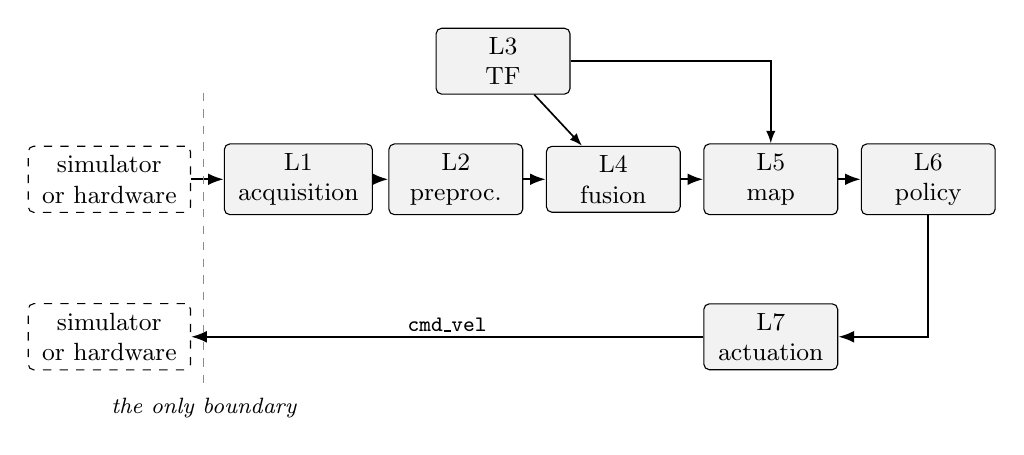
\begin{tikzpicture}[x=1cm, y=1cm,
                      lyr/.append style={minimum width=17mm},
                      ext/.append style={minimum width=20mm}]
    \node[lyr] (l3) at (5.0,1.5) {L3\\TF};

    \node[ext] (win) at (0,0)   {simulator\\or hardware};
    \node[lyr] (l1)  at (2.4,0) {L1\\acquisition};
    \node[lyr] (l2)  at (4.4,0) {L2\\preproc.};
    \node[lyr] (l4)  at (6.4,0) {L4\\fusion};
    \node[lyr] (l5)  at (8.4,0) {L5\\map};
    \node[lyr] (l6)  at (10.4,0){L6\\policy};

    \draw[flow] (win) -- (l1);
    \draw[flow] (l1) -- (l2);
    \draw[flow] (l2) -- (l4);
    \draw[flow] (l4) -- (l5);
    \draw[flow] (l5) -- (l6);

    \draw[thin flow] (l3) -- (l4);
    \draw[thin flow] (l3) -| (l5);

    \node[lyr] (l7)  at (8.4,-2)  {L7\\actuation};
    \node[ext] (wout) at (0,-2)   {simulator\\or hardware};
    \draw[flow] (l6.south) |- (l7.east);
    \draw[flow] (l7.west) -- node[lbl,above]{\texttt{cmd\_vel}} (wout.east);

    \draw[dashed, black!45] (1.2,1.1) -- (1.2,-2.6);
    \node[note, anchor=north] at (1.2,-2.65) {the only boundary};
  \end{tikzpicture}
  \caption{The chain of guarantees of Section~\ref{sec:pipeline-architecture}.
           Each layer assures the next a property that allows it to disregard
           everything upstream: L4 receives a filtered cloud and does not know
           which device produced it, and L6 receives occupancy and does not know
           which engine built it. L3 publishes the common geometry rather than
           sitting on the path, and L7 makes the command observable without
           being interposed on it.}
  \label{fig:pipeline-chain}
\end{figure}

\section{Pipeline Architecture}
\label{sec:pipeline-architecture}

The chain may be read as a succession of guarantees: each layer assures the next
one a property that allows it to disregard everything that precedes it. It is
this chain of guarantees, rather than the sequence of nodes, that makes the
system independent of the platform.

The first layer guarantees \emph{uniformity of form}. Devices of the same type
do not necessarily expose the same streams: a depth camera may provide the point
cloud already computed or only the depth image, and a camera may provide
rectified or raw images. Since the subsequent layers are designed for a single
case, the first layer reconstructs whatever the device does not provide, so that
downstream every type of datum always appears in the same form. A distinct case
is kept separate from this mechanism, namely one in which a capability does not
exist at all on the platform under consideration: the system keeps explicit the
difference between a stream that can be derived and one that no node is able to
produce, so that the absence of a capability is not interpreted downstream as a
fault.

The second layer guarantees \emph{declared reliability}. Every datum is checked
for plausibility and continuity, is reduced to what is useful downstream, and
above all is accompanied by the judgement the system forms about it. That
judgement does not remain a diagnostic annotation: it determines the decision
uniquely --- publication, publication with increased uncertainty, or
rejection --- and is conveyed downstream in the covariance matrix that
accompanies the measurement. Without an explicit declaration of reliability the
subsequent layers would have no criterion by which to distinguish a trustworthy
measurement from a compromised one. The layer produces no estimate and does not
cross-check sensors: each node observes a single device, and any processing that
requires a comparison between sources belongs to the fusion layer.

The third layer, TF, guarantees a \emph{common geometry}. Since every device measures
in its own reference frame, comparing and fusing heterogeneous measurements
requires those frames to be related to that of the vehicle. The relations
between the body and the sensors are static and derive from the same mounting
declaration used to build the model of the robot in simulation. To them are
added the two dynamic relations prescribed by the conventional model adopted in
ROS~2: the one between the odometry origin and the body, continuous but subject
to drift, and the one between the world frame and the odometry origin, corrected
but discontinuous. The distinction has a direct operational consequence, since
short-term motion control relies on the continuous frame, whereas localisation
in the environment relies on the corrected one.

The fourth and fifth layers guarantee the \emph{unified products} --- one pose
and one representation of the environment --- and are treated respectively in
Section~\ref{sec:pipeline-fusion} and Section~\ref{sec:observation-space}, since
both contribute to defining what the network observes.

The seventh layer, finally, guarantees the \emph{observability of the command}.
It is not interposed on the path that carries the command to the actuators, but
republishes it time-stamped and at a constant rate, even in the absence of new
commands. It thereby becomes possible to determine which command was in force at
a given instant, a property on which the recording of the training corpus
depends (Section~\ref{sec:observation-recording}).

Two conventions, lastly, cut across all layers. The naming of the channels
declares the point of the chain at which the datum stands and the node that
produced it, and is constructed by a single shared module, since a divergence in
naming would not raise any detectable error, but the silent absence of
communication between two components. Uncertainty, as observed above,
constitutes the language in which sources are weighed against one another: from
that convention follows a property that conditions the design of the fusion
layer, namely that a source declaring an untruthful uncertainty degrades the
estimate more than its absence would.

\section{Multi-Sensor Data Fusion}
\label{sec:pipeline-fusion}

The fourth layer is the first in which measurements from different sensors are
compared. From that comparison derive the two unified products on which the rest
of the system rests: the pose, that is a single estimate of the state of the
vehicle, and a single point cloud expressed in the body frame, obtained by
temporally aligning the measurements of sources that differ in field of view,
range, density and rate.

The estimates produced by the individual sources are collected by a recursive
Bayesian filter, which maintains the state of the vehicle and corrects it at
every incoming measurement, weighing it by its own uncertainty. Since the
weighing rests on the declared covariance, the correctness of that declaration
directly conditions the quality of the estimate: many odometry implementations
leave the covariance field at zero, not because the estimate is exact but
because they do not compute its uncertainty, and the filter interprets the zero
value as certainty, anchoring itself to it and disregarding the remaining
sources. The layer therefore comprises a family of nodes whose task is to
attribute to the estimates the uncertainty they do not declare, modulating it
wherever a measurable quantity exists on which to base the attribution --- as in
the case of a geometrically degenerate environment, which makes one direction of
motion unobservable, or of wheel slippage, which invalidates the odometry
derived from it --- and declaring it constant elsewhere, since in the absence of
any evidence a declared constant is preferable to an arbitrary modulation.

It remains to be established, when several sources observe the same quantities,
which of them determines each component of the state. A criterion founded on
accuracy would require the sources to be ordered from the most precise to the
least precise, and that ordering to be recalibrated for every combination of
platform, terrain and environment, which would contradict the principle of
platform independence stated in Section~\ref{sec:pipeline-overview}. The system
therefore adopts a criterion founded on the \emph{type} of measurement, which is
a stable property of the device and not of the environment in which it operates:
direct velocity measurements are all admitted, since they do not compete with
one another and weighing them is the filter's task; external references not
subject to drift acquire ownership of the dimension they observe, and no
estimate obtained by integration may displace them; integrated estimates cover
the remaining dimensions, and those not elected contribute their own increments
rather than imposing their own pose. The configuration of the filter is
generated from that policy on the basis of the declared set of sensors, and
verified against a set of invariants that make structurally impossible the error
conditions the filter would otherwise report at run time.

\section{Observation Space}
\label{sec:observation-space}

This section defines the input of the network. It is the point at which the
pipeline ceases to be a perception system and becomes the contract on which
Chapter~\ref{ch:lnn} rests: every quantity listed here is a quantity the network
observes, and every representational choice made here is a choice the training
inherits.

\subsection{From the local map to the ego-centric crop}
\label{sec:observation-map}

The fifth layer builds two representations of the environment, distinct in
purpose and in requirements. The global map maintains the long-term consistency
of the space traversed and is used to correct the drift of the odometry through
the recognition of places already visited. The local map represents the space
immediately surrounding the vehicle as a grid of occupied voxels, and only the
latter reaches the network. The substantial difference lies in memory: the
global map must retain, whereas the local map must forget, since an obstacle
that has moved must disappear quickly and a cumulative representation would
populate the space with obstacles that no longer exist. It is a property
required by the use the network makes of it: the learnt policy reacts to what
surrounds the vehicle at the current instant, and a residual obstacle would be
indistinguishable from a real one.

The last node of the layer prepares the input of the network
(Figure~\ref{fig:observation}): the occupied voxels are brought into the body
frame of the robot and cropped within a sphere of fixed radius, bounded above
and below in height. Two choices deserve to be motivated. Expressing them in the
body frame keeps the coordinates bounded, preventing them from growing with the
distance travelled and making the observation invariant with respect to the
absolute position of the vehicle in the environment. The spherical shape, in
place of the rectangular volume in which the map is built, answers a requirement
of directional uniformity: in a rectangular volume the distance from the centre
depends on the direction, so that the network would receive a field of
observation varying with orientation, that is a systematic distortion that would
be learnt along with the behaviour. The crop is three-dimensional --- the radius
is measured in space, and the horizontal section therefore narrows towards the
top --- while the bounds in height remain independent of the radius, since the
space usable by a platform is limited in elevation.

\begin{figure}[htbp]
  \centering
  \linespread{1}\selectfont
  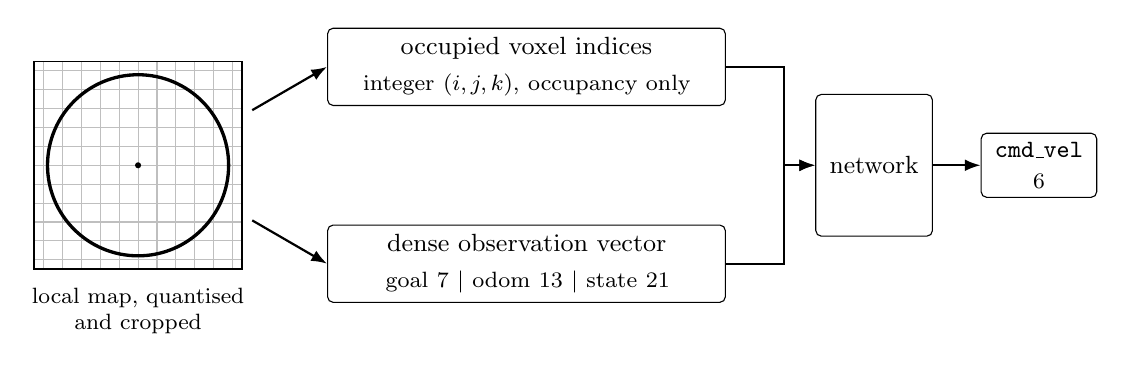
\begin{tikzpicture}[x=1cm, y=1cm]
    \draw[black!25, step=2.4mm] (-1.32,-1.32) grid (1.32,1.32);
    \draw[semithick] (-1.32,-1.32) rectangle (1.32,1.32);
    \draw[very thick] (0,0) circle (1.15);
    \fill (0,0) circle (1.1pt);
    \node[lbl, anchor=north] at (0,-1.5) {local map, quantised\\and cropped};

    \node[blk, anchor=west, text width=47mm] (coords) at (2.4,1.25)
      {occupied voxel indices\\[2pt]\footnotesize integer $(i,j,k)$, occupancy only};
    \node[blk, anchor=west, text width=47mm] (dense) at (2.4,-1.25)
      {dense observation vector\\[2pt]\footnotesize goal 7 $\mid$ odom 13 $\mid$ state 21};

    \draw[flow] (1.45,0.7) -- (coords.west);
    \draw[flow] (1.45,-0.7) -- (dense.west);

    \node[blk, minimum height=18mm, anchor=west] (net) at (8.6,0) {network};
    \draw[flow] (coords.east) -| ([xshift=-4mm]net.west) -- (net.west);
    \draw[flow] (dense.east)  -| ([xshift=-4mm]net.west) -- (net.west);

    \node[blk, anchor=west] (cmd) at (10.7,0) {\texttt{cmd\_vel}\\\footnotesize 6};
    \draw[flow] (net) -- (cmd);
  \end{tikzpicture}
  \caption{What the network observes. The local map is cropped into a sphere
           expressed in the body frame and quantised on a grid of the same pitch
           it was built with, reaching the network as the integer indices of the
           occupied cells --- occupancy alone, with no trace of the sensor that
           measured it. Beside it travels the dense vector of
           Table~\ref{tab:obs}, whose third block declares the body.}
  \label{fig:observation}
\end{figure}

\subsection{The representation of the cloud}
\label{sec:observation-cloud}

The cropped cloud is quantised on a grid aligned with the body axes, with the
same pitch used in the construction of the map, and delivered to the network as
a set of integer indices of the occupied voxels rather than as a set of
continuous coordinates. The representation is therefore purely binary: the
network observes which cells of the surrounding space are occupied, and neither
the density of the points that occupy them nor any photometric attribute. It
follows that the nature of the sensor that produced the measurement is not
observable by the network, which extends to the input of the policy the property
of platform independence that governs the whole pipeline.

The quantisation pitch and the crop radius are not redeclared at this level, but
read from the configuration of the nodes that actually applied them. The reason
is that quantising with a pitch different from the one with which the map was
built would produce no detectable error, but rather an input foreign to the
distribution on which the network was trained. The two parameters moreover vary
across platforms, and with them varies the extent of the grid: the corpus used
in this work comprises four of them, a circumstance the training accounts for by
stratifying the data split on the voxel pitch (Section~\ref{sec:sl-split}),
since a convolutional operator of fixed size covers a different physical extent
at a different resolution.

\subsection{The dense observation vector}
\label{sec:observation-vector}

Alongside the cloud the network receives a vector of \num{41} floating-point
values, organised in three blocks (Table~\ref{tab:obs}).

\begin{table}[H]
  \centering
  \caption{Composition of the dense observation vector.}
  \label{tab:obs}
  \begin{tabular}{@{}llp{7.2cm}@{}}
    \toprule
    \textbf{Block} & \textbf{Dim.} & \textbf{Content} \\
    \midrule
    Goal     & 7  & position and orientation of the assigned goal \\
    Odometry & 13 & position, orientation, linear velocity and angular velocity, from the fused pose \\
    State    & 21 & geometry and mass of the body (7), kinematic limits (12), voxel pitch (1), model identifier (1) \\
    \midrule
    \textbf{Total} & \textbf{41} & \\
    \bottomrule
  \end{tabular}
\end{table}

The first block is the goal, which the system receives from an operator or from
the mission configuration, expressed in the same frame as the pose: the network
therefore observes the goal and its own placement, and not the vector separating
them, whose construction is left to the network itself. The second block is the
pose produced by the fourth layer, with the linear and angular velocities that
accompany its estimate.

The third block is the element that makes a single network usable on a
heterogeneous fleet, and deserves to be examined in its components. The first
seven describe the body of the vehicle --- extent, centre of mass and mass ---
and thus place the dynamics of the robot within the observation. The following
twelve are the kinematic limits declared by the platform: minimum and maximum
velocity and acceleration on the linear, angular and vertical channels. They
constitute the scale with respect to which a command is to be interpreted, since
the same absolute velocity represents a moderate command on one platform and a
command at the limit on another; their role extends beyond the observation, in
that the loss function of supervised training uses them to make comparable the
errors committed on different robots (Section~\ref{sec:sl-loss}). A null limit,
moreover, declares that the corresponding axis does not exist on the platform,
as vertical velocity on a ground vehicle: the observation is therefore able to
represent the absence of a degree of freedom without the structure of the vector
changing.

The last two components declare the voxel pitch of the map --- which informs the
network of the resolution at which the concurrent cloud was built --- and the
identifier of the robot model. The latter is a categorical variable rather than
a physical quantity, and the treatment it receives inside the network is
discussed in Section~\ref{sec:aux-modules}.

The output is a six-component velocity command --- three linear and three
angular velocities --- expressed in the physical units of the platform and
published on the command channel of the vehicle, the same on which an operator
would publish. Nothing along this path saturates the command against the limits
declared in the third block: limiting, where necessary, is the task of the
on-board controller, and the network is evaluated on what it actually commands.

\subsection{Recording the corpus}
\label{sec:observation-recording}

The three components that consume the contract just defined --- the node that
records the corpus, the node that runs inference on board and the interface
towards the reinforcement learning environment --- share a single
implementation. The network is in fact trained on what the first produces and
executed inside the other two, and distinct implementations of the same
definition would diverge without raising any error, since the dimensions of the
vectors would continue to match and the only observable effect would be
erroneous behaviour.

Recording pairs in time the observation available to the vehicle with the action
that followed from it. The pairing is not symmetric: the pose is sought in the
neighbourhood of the instant of the observation, since it describes the state
the vehicle was in, whereas the command is sought \emph{afterwards}, since it
constitutes the reaction to it. The command considered is the one republished by
the seventh layer, whose re-emission at a constant rate makes it determinable
which command was in force at each instant, even when the operator has issued no
new ones. Every sample is moreover stamped with its own instant of acquisition:
the interval between consecutive samples is not constant, and constitutes in
turn an input of the network, for the reasons set out in
Section~\ref{sec:lnn-taxonomy}.

\section{Simulation--Hardware Parity}
\label{sec:pipeline-parity}

The system is designed so that simulation and real hardware are
interchangeable. The boundary between the two cases crosses the chain at a
single point, constituted by the boundary channels of the vehicle: on them
publishes the bridge towards the simulator when the robot is simulated, and the
driver of the device when it is real, while the command traverses the same
frontier in the opposite direction. Downstream of that point the nodes are the
same and hold no information about the origin of the data.

The two cases differ in the naming of the boundary channels alone: in simulation
it is established by the project, whereas with real hardware it is imposed by
the manufacturer of the device, in the absence of a common convention among
vendors. The difference is absorbed at a single point of the configuration, in
which the channel on which each stream actually arrives is declared. Moving to
real hardware therefore entails a change in three elements only --- the
component that publishes on the boundary channels, the source of time, and the
generated configuration --- while the seven layers, the frame tree, the tuning
parameters of the nodes and the fusion policy remain unchanged.

The property is essential to this work in two respects. The first concerns the
data: the training corpus is recorded through the same chain that will feed the
network during execution, so that the observation on which the policy is trained
and the one it receives on board are produced by the same code. The second
concerns geometry: since the model used in simulation and the static transforms
derive from the same mounting declaration, the geometry assumed by the system
and the one realised by the simulator coincide by construction, and the
discrepancy between simulation and reality does not include, at least, the
placement of the sensors.

%!TEX root = ../main.tex
\chapter{Liquid Neural Networks}
\label{ch:lnn}

\section{Overview}
\label{sec:lnn-overview}

The network this work trains takes the place of the pilot: it receives the
observation defined in Section~\ref{sec:observation-space} --- the local voxel
map, the pose, the goal and the declaration the robot makes about itself --- and
produces the velocity command the platform executes. The problem has three
properties that determine the architecture.

It is \emph{partially observable}: a single frame does not say whether the robot
was accelerating, whether the obstacle ahead is approaching, or how long it has
been standing still. Memory is therefore expected to help --- an expectation,
not a premise, which the stateless control of
Section~\ref{sec:networks-implementation} exists to test.

It is \emph{non-uniform in time}: the rate at which frames arrive is not
constant. A discrete-time recurrent network, such as an LSTM
\cite{hochreiter1997lstm} or a GRU \cite{cho2014gru}, treats every step as
equivalent to the previous one, and therefore interprets a two-second
interruption as though it were an interval of a tenth of a second. This is the
reason why the family of cells adopted is that of \emph{Liquid Neural Networks}
\cite{hasani2021ltc,hasani2022cfc}: the state evolves not by iteration but by
integration of a differential equation, and the elapsed time is an input of the
update rather than an implicit assumption. The same family has been employed
successfully in end-to-end learnt flight navigation \cite{chahine2023flight},
which shares with the present problem the nature of the input and the need to
generalise outside the training distribution.

It is, finally, \emph{heterogeneous}: the same network must fly different
platforms, with velocity limits that vary and masses that differ. The
architecture therefore contains two modules --- the observation normaliser and
the robot-model embedding --- whose task is to make comparable robots that are
not.

\paragraph{The structure.}
The architecture is a single one, with two points of variation
(Figure~\ref{fig:architecture}). Three
independent branches --- the sparse encoder that reduces the voxel map to a
compact descriptor, the normalisation of the \num{41} dense values, and the
robot-model embedding --- are concatenated and projected by a single linear
layer into a fusion vector. The fusion vector traverses two recurrent cells in
cascade, and the state of the second feeds a linear head that produces the six
components of the command, rescaled by a final affine stage. The two points of
variation are \emph{which cell} occupies the recurrent core --- LTC, CfC or
LRCU --- and \emph{whether that core is sparsely wired} according to the NCP
scheme. Everything else lives in a common base class and is identical across all
variants, so that a change to the input or output path reaches every variant at
once and the comparison isolates exactly the two choices.

\begin{figure}[htbp]
  \centering
  \linespread{1}\selectfont
  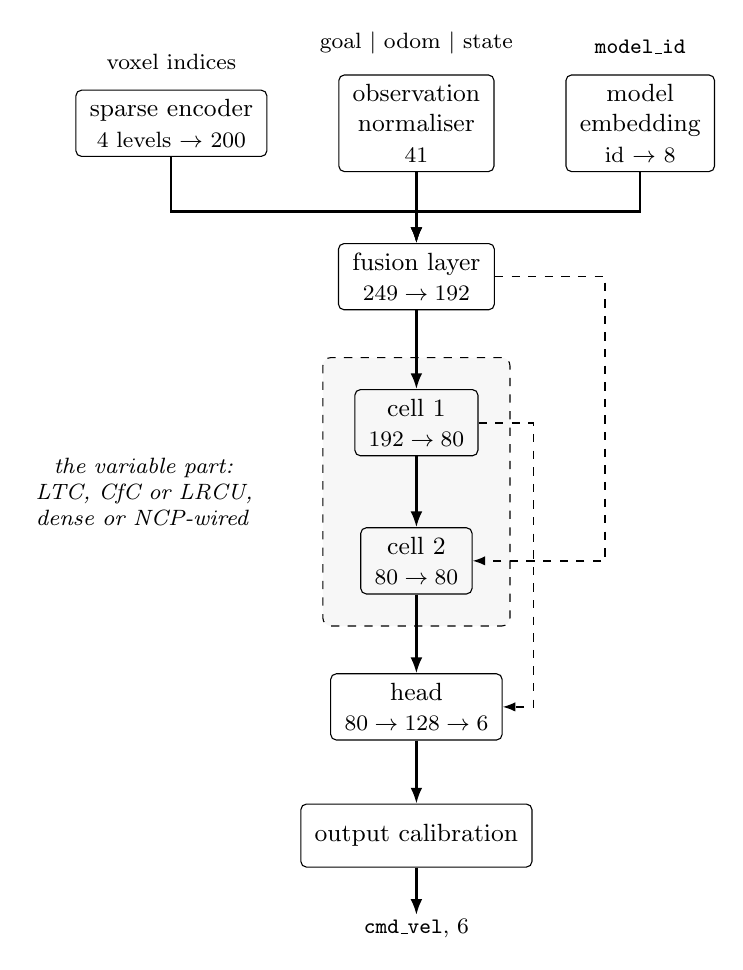
\begin{tikzpicture}[node distance=6mm]
    \node[blk] (enc) {sparse encoder\\\footnotesize 4 levels $\to$ 200};
    \node[blk, right=9mm of enc] (nrm) {observation\\normaliser\\\footnotesize 41};
    \node[blk, right=9mm of nrm] (emb) {model\\embedding\\\footnotesize id $\to$ 8};

    \node[lbl, above=2mm of enc] {voxel indices};
    \node[lbl, above=2mm of nrm] {goal $\mid$ odom $\mid$ state};
    \node[lbl, above=2mm of emb] {\texttt{model\_id}};

    \node[blk, below=9mm of nrm] (fus) {fusion layer\\\footnotesize $249 \to 192$};
    \draw[flow] (enc.south) |- ([yshift=4mm]fus.north) -- (fus.north);
    \draw[flow] (nrm) -- (fus);
    \draw[flow] (emb.south) |- ([yshift=4mm]fus.north) -- (fus.north);

    \node[blk, below=10mm of fus] (c1) {cell 1\\\footnotesize $192 \to 80$};
    \node[blk, below=9mm of c1]  (c2) {cell 2\\\footnotesize $80 \to 80$};
    \draw[flow] (fus) -- (c1);
    \draw[flow] (c1) -- (c2);

    \begin{scope}[on background layer]
      \node[draw, dashed, rounded corners=3pt, fill=black!3,
            fit=(c1)(c2), inner sep=4mm] (core) {};
    \end{scope}
    \node[note, left=8mm of core, text width=27mm, anchor=east]
      {the variable part:\\LTC, CfC or LRCU,\\dense or NCP-wired};

    \node[blk, below=10mm of c2] (head) {head\\\footnotesize $80 \to 128 \to 6$};
    \node[blk, below=8mm of head] (cal) {output calibration};
    \node[lbl, below=6mm of cal] (out) {\texttt{cmd\_vel}, 6};
    \draw[flow] (c2) -- (head);
    \draw[flow] (head) -- (cal);
    \draw[flow] (cal) -- (out);

    \draw[thin flow, dashed] (fus.east) -- ++(14mm,0) |- (c2.east);
    \draw[thin flow, dashed] (c1.east)  -- ++(7mm,0)  |- (head.east);
  \end{tikzpicture}
  \caption{The architecture, with the two points of variation. Everything
           outside the dashed box is common to all the networks compared; inside
           it sit the two recurrent cells, which differ in their update rule and
           in whether their matrices are masked. The dashed arrows on the right
           are the two bypass paths that only the sparsely wired variants carry
           (Section~\ref{sec:lnn-wiring}).}
  \label{fig:architecture}
\end{figure}

\section{Continuous-Time Cells: LTC, CfC and LRCU}
\label{sec:lnn-taxonomy}

\subsection{From neural differential equations to liquid cells}
\label{sec:lnn-background}

The three cells employed in this work belong to a single line of models, and
understanding them requires that line to be briefly retraced.

The point of departure is the family of \emph{neural ordinary differential
equations} \cite{chen2018neuralode}, in which the hidden state
$x(t) \in \mathbb{R}^{D}$ is not updated by a discrete recurrence but defined as
the solution of
\begin{equation}
  \frac{\mathrm{d}x(t)}{\mathrm{d}t} = f\!\left(x(t), I(t), t, \theta\right),
  \label{eq:node}
\end{equation}
where $I(t)$ is the input and $f$ a neural network with parameters $\theta$. The
state at an arbitrary instant is obtained by numerically integrating
Equation~\eqref{eq:node}, and the network is trained by differentiating through
the solver. The formulation makes the model naturally defined on a continuous
time axis, but offers no guarantee on the asymptotic behaviour of the state.

A more stable formulation is that of \emph{continuous-time recurrent networks}
\cite{funahashi1993ctrnn}, which add to the learnt term an exponential decay
towards equilibrium,
\begin{equation}
  \frac{\mathrm{d}x(t)}{\mathrm{d}t}
    = -\frac{x(t)}{\tau} + f\!\left(x(t), I(t), t, \theta\right),
  \label{eq:ctrnn}
\end{equation}
in which $\tau$ is a time constant governing the speed at which the autonomous
system reaches equilibrium. The time constant is, however, a fixed parameter:
every unit forgets at the same speed, whatever it is observing.

The contribution of liquid cells consists in making that speed \emph{dependent
on the input and on the state}. The three cells compared in this work realise
the idea in three different ways: LTC by explicitly modulating the time constant
of the differential equation, CfC by replacing numerical integration with a
closed-form approximation of its solution, and LRCU by making variable the
capacitance of the equivalent circuit from which the equation derives. A
systematic comparison of the family against classical recurrent networks, on
accuracy, memory footprint and generalisation, is reported in
\cite{zong2025lnnsurvey}; the same line of research has since been extended to
structured state-space models \cite{hasani2023liquids4}, which are not employed
in this work.

\subsection{Liquid Time-Constant (LTC)}
\label{sec:cell-ltc}

The LTC cell \cite{hasani2021ltc} originates in an observation about the
dynamics of non-spiking neurons: the membrane potential evolves as a first-order
linear system, while the synaptic currents entering it are, in the steady state,
a sigmoidal nonlinearity of the state of the presynaptic neurons, multiplied by
the difference between the current potential and a reference potential $A$.
Substituting that term into Equation~\eqref{eq:ctrnn} yields
\begin{equation}
  \frac{\mathrm{d}x(t)}{\mathrm{d}t}
    = -\left[\frac{1}{\tau} + f\!\left(x(t), I(t), t, \theta\right)\right] x(t)
      + f\!\left(x(t), I(t), t, \theta\right) A .
  \label{eq:ltc}
\end{equation}

The difference with respect to Equation~\eqref{eq:ctrnn} is substantial. The
network $f$ no longer determines only the derivative of the state, but appears
also in the coefficient multiplying the state itself: it therefore acts as a
variable time constant of the system,
\begin{equation}
  \tau_{\text{sys}}
    = \frac{\tau}{1 + \tau f\!\left(x(t), I(t), t, \theta\right)} ,
  \label{eq:tausys}
\end{equation}
and it is from this dependence that the adjective \emph{liquid} derives. Each
unit of the hidden state may thus specialise on a time scale of its own and
modify it according to what it observes --- reacting quickly to an input that
changes, and retaining for a long time an information that does not --- whereas
Equation~\eqref{eq:ctrnn} would impose the same speed in both cases.

The model enjoys two properties proved in \cite{hasani2021ltc} that motivate its
use in a control loop. The first is that the time constant remains bounded,
$\tau/(1 + \tau W) \le \tau_{\text{sys}} \le \tau$, where $W$ collects the
weights entering the unit under consideration; the second is that the state of
each unit remains confined between $\min(0, A_{\min})$ and $\max(0, A_{\max})$
over any finite interval, whatever the magnitude of the input. The second
property is of greater practical relevance: the output of the recurrent core
cannot diverge even when the observation contains anomalous values, a condition
that in a real system occurs whenever a source of odometry degrades.

Equation~\eqref{eq:ltc} admits no analytical solution and constitutes a
\emph{stiff} system of equations, for which a Runge--Kutta integrator would
require a prohibitive number of steps. The authors therefore propose a
\emph{fused} solver, which replaces with the updated value only the occurrences
of the state that appear linearly, and can thus be solved symbolically,
obtaining the stability of the implicit Euler method at the cost of the explicit
one:
\begin{equation}
  x(t + \Delta t)
    = \frac{x(t) + \Delta t\, f\!\left(x(t), I(t), t, \theta\right) \odot A}
           {1 + \Delta t\left[1/\tau + f\!\left(x(t), I(t), t, \theta\right)\right]} .
  \label{eq:ltc-fused}
\end{equation}

\paragraph{In the implementation.}
Equation~\eqref{eq:ltc-fused} is realised as written, with
$f = \sigma(W_{\text{in}} u + W_{\text{rec}} x + b)$, with $\tau$ obtained as
$\operatorname{softplus}(\tau_{\text{raw}})$ so as to guarantee its positivity,
and with $A$ learnt. The step $\Delta t$ is fixed when the cell is constructed
and repeated a configurable number of times per input step, following the
\emph{unfolding} scheme prescribed by the authors. The initialisation of
$\tau_{\text{raw}}$ places the time constants on an interval comparable with the
rate of the data, so that the cell integrates meaningfully from the first step.

\subsection{Closed-form Continuous-time (CfC)}
\label{sec:cell-cfc}

The use of a numerical solver, however efficient, remains the principal cost of
continuous-time cells: every forward step requires one or more evaluations of
the differential equation, and the cost is multiplied by the length of the
sequence. The CfC cell \cite{hasani2022cfc} removes that cost by replacing the
integration with a \emph{closed-form approximation} of the solution of
Equation~\eqref{eq:ltc}, for which no analytical expression was previously
known. The authors report a speed-up of between one and five orders of
magnitude, in training and in inference, with respect to the equivalent
solver-based models.

The approximate solution takes the form
\begin{equation}
  x(t) = \sigma\!\left(-f(x, I; \theta_f)\, t\right) \odot g(x, I; \theta_g)
       + \left[1 - \sigma\!\left(-f(x, I; \theta_f)\, t\right)\right] \odot h(x, I; \theta_h),
  \label{eq:cfc}
\end{equation}
where $f$, $g$ and $h$ are three neural networks and $\sigma$ is the sigmoid.
The reading of Equation~\eqref{eq:cfc} is immediate: $g$ and $h$ describe
respectively the initial and the asymptotic behaviour of the unit, while the
sigmoid interpolates between the two as a function of the elapsed time, with a
transition speed determined by $f$, that is by the input and the state. Time
appears here \emph{explicitly} as an argument, and not as a discretisation step:
it is this property that makes the cell suited to a stream of observations at an
irregular rate, since a long interval and a short one produce by construction
two different values of the same gate.

\paragraph{In the implementation.}
The three networks share a common backbone, following the realisation proposed
by the authors: a single layer $s = \tanh(W [\,u, x\,] + b)$ produces a hidden
vector that three linear heads read, so that the cost of the cell remains close
to that of a traditional recurrence. The gate takes the form
$\gamma = \sigma\!\left(-\left(w_\tau + f(s)\right)\Delta t\right)$, in which
$w_\tau$ is a per-unit learnt time constant, and the updated state is
$x' = \gamma \odot g(s) + (1 - \gamma) \odot h(s)$.

The initialisation of $w_\tau$ deserves a remark, since it determines whether
the cell behaves as a continuous-time model at all. Set to zero, with a rate of
the order of a tenth of a second, the argument of the gate starts within a
hundredth of zero: the sigmoid pins the gate at $0.5$, the cell degenerates into
a constant blend of two heads, and the time constant for which it exists plays
no part. The initialisation adopted is therefore log-uniform over an interval of
time constants physically sensible for the problem --- $w_\tau$ is a rate, hence
the reciprocal of a time --- and places the gate in a usable region from the
first step.

\subsection{Liquid Resistance-Capacitance Unit (LRCU)}
\label{sec:cell-lrcu}

The third cell descends from the same equivalent electrical circuit from which
LTC moves, but revises two of its simplifications. The first concerns
saturation: in Equation~\eqref{eq:ltc} the synaptic conductance is not bounded
from above, whereas in a real circuit it is; saturated-conductance models
reintroduce the bound. The second, which constitutes the contribution proper to
\emph{liquid-resistance liquid-capacitance} networks \cite{farsang2024lrc},
concerns the membrane capacitance: in LTC it is constant, and only the
resistance varies with the state. Making the capacitance variable as well yields
\begin{equation}
  \frac{\mathrm{d}x}{\mathrm{d}t}
    = \varepsilon(w) \odot \left[-\,\sigma(f)\odot x + \tau(u) \odot e_{\ell}\right],
  \label{eq:lrc}
\end{equation}
where $\sigma(f)$ is the forget conductance, $\tau(u)$ the update conductance
towards the resting potential $e_{\ell}$, and $\varepsilon(w)$ is the
\emph{liquid elastance}, the reciprocal of the capacitance, itself a function of
the input and of the state. The third factor acts on the whole derivative: it
does not establish \emph{towards what} the unit evolves, but \emph{how quickly}
it does so, and is therefore a second mechanism of temporal modulation added to
the one already present in LTC.

The authors observe that integrating Equation~\eqref{eq:lrc} with an explicit
Euler method of order one and a single unfolding step yields a discrete
recurrence --- the LRCU unit --- structurally akin to a gated RNN, in which
$\varepsilon$ plays the role of the update gate of a GRU \cite{cho2014gru},
with in addition the conductance structure of the circuit from which it derives.
It is in this form that the cell is employed in the present work, since it
thereby retains the cost of a traditional recurrence.

\paragraph{In the implementation.}
The update is
\begin{equation}
  x' = x + \Delta t\, \varepsilon \odot
       \left(-f \odot x + z \odot e_{\ell}\right),
  \label{eq:lrcu}
\end{equation}
with the three quantities computed as
\begin{align}
  f           &= \operatorname{softplus}(g_{\max}) \odot \sigma\!\left(W^{\text{in}}_f u + W^{\text{rec}}_f x + b_f\right), \\
  z           &= \operatorname{softplus}(k_{\max}) \odot \sigma\!\left(W^{\text{in}}_z u + W^{\text{rec}}_z x + b_z\right), \\
  \varepsilon &= \sigma\!\left(W^{\text{in}}_\varepsilon u + w_\varepsilon \odot x + v_\varepsilon\right).
\end{align}
The forget and update conductances are therefore sigmoids scaled by a learnt
maximum conductance, according to the saturated form discussed above, while the
elastance has a diagonal rather than a full recurrence. The cell holds three
input matrices and two complete recurrent matrices, and is for this reason the
most expensive of the three at equal state width: the comparison of
Chapter~\ref{ch:results} is to be read bearing that asymmetry in mind, as
reported in Table~\ref{tab:architectures}.

\subsection{Time, and the asymmetry it introduces}
\label{sec:cell-time}

The three cells treat time in two distinct ways, and the difference must be
declared because it bears on the comparison. In the CfC the elapsed time appears
explicitly in Equation~\eqref{eq:cfc} as the argument of the gate: the cell
therefore receives the \emph{real} $\Delta t$ between two consecutive
observations and adapts its transition to it. In LTC and LRCU time appears
instead as the discretisation step of a numerical integration
(Equations~\eqref{eq:ltc-fused} and~\eqref{eq:lrcu}), fixed when the cell is
constructed; the real $\Delta t$ reaches them as an additional component of the
input, which is the reason why their observation vector is \num{42} values wide
rather than \num{41}.

The asymmetry is a consequence of the formulation and not a choice of the
implementation. Since the rate of the observations is not constant
(Section~\ref{sec:observation-recording}), the constant step is inexact for a
non-negligible fraction of the samples, and the same quantity reaches the CfC in
a more informative form than that in which it reaches the other two. Supplying
LTC and LRCU with a per-sample integration step would alter their update rule
--- and, in the case of LTC, would invalidate the stability bounds recalled in
Section~\ref{sec:cell-ltc}, which presuppose a fixed step --- so that the
comparison would be between a cell and a variant of it, rather than between the
cells proposed in the literature.

\section{Wiring: Dense and NCP}
\label{sec:lnn-wiring}

The second choice concerns the connectivity of the recurrent core. In the dense
variants every weight matrix is full and the cascade is direct: fusion, first
cell, second cell, head.

The alternative variants draw on \emph{Neural Circuit Policies}
\cite{lechner2020ncp}, in which a continuous-time cell is embedded in a sparse
wiring derived from the nervous system of the nematode \emph{Caenorhabditis
elegans}. The original wiring organises the neurons in four groups ---
sensory neurons, interneurons, command neurons and motor neurons --- with sparse
connections between adjacent groups, recurrence concentrated in the command
group, and synapses whose sign, excitatory or inhibitory, is established by the
structure of the circuit rather than learnt. The authors show that an end-to-end
driving policy can be realised with \num{19} control neurons and \num{253}
synapses, and attribute to such compactness three advantages: interpretability
of the learnt policy, robustness with respect to perturbations of the input, and
a reduction of the parameter space.

Of that approach the present work adopts the two elements that can be applied to
a recurrent core of fixed width without redesigning its topology. The first is
\emph{signed sparsity}: the matrices of each cell are multiplied by a mask
generated at initialisation, which removes a fraction of the connections and
assigns to each of the remaining ones a constant sign that training cannot
reverse. The density is \num{0.6} on the input connections and \num{0.8} on the
recurrent ones. The masks are registered as buffers and are therefore part of
the checkpoint, so that a reloaded network resumes exactly the connectivity with
which it was trained. The second is the presence of \emph{paths that bypass one
level}, analogous to the diagonal connections of the biological circuit: from
the input to the second cell, and from the first cell to the head, both at
density \num{0.4}. The former is supported natively by the cells; the latter,
since the head is a linear layer and not a cell, is realised as a separate
masked additive path, leaving the main weights of the head dense.

The four-group topology of the original wiring is not adopted. The reason is
that the architecture described in this chapter places the recurrent core
between a convolutional encoder and a calibrated head, both dense and common to
all variants: introducing a sensory group and a motor group would mean modifying
the input and output paths as well, and the comparison would no longer isolate
connectivity alone. What the sparse variants of this work measure is therefore
the contribution of signed sparsity and of the bypass paths, not that of the
complete circuit proposed in \cite{lechner2020ncp}; the designation NCP is
retained for continuity with the literature and with the implementation, but is
to be understood in this restricted sense.

The dense variants have neither masks nor bypass paths, and are identical in
everything else --- encoder included --- to their sparse counterpart. The pair
therefore isolates exactly what sparsity and the bypass paths are worth.

\section{Sparse Convolutional Encoder}
\label{sec:sparse-encoder}

The encoder reduces the local voxel map to a descriptor of fixed length. It is a
four-level pyramid of \num{16}, \num{24}, \num{32} and \num{48} channels, each
preceded from the second onwards by a downsampling stage of stride~\num{2}. The
convolutions are \emph{submanifold} \cite{graham2018submanifold}, that is they
keep the computation anchored to the occupied voxels alone instead of densifying
the grid: it is the property that makes tractable an input in which almost all
cells are empty. Every level
is pooled per sample by a reduction over the active sites, and the four
descriptors are concatenated into a vector of \num{200} channels.

Two normalisation choices deserve to be motivated, since neither follows from
the pyramid itself. The first is the use of \emph{group normalisation} in place
of \emph{batch normalisation}. Batch statistics would here be computed over the
active voxels of whatever samples share a batch, and the number of active voxels
varies appreciably from one recording to another: the statistics would therefore
depend on the composition of the batch rather than on the scene, and the
descriptor produced for a fixed input would move from one epoch to the next.
Group normalisation removes that dependence, since it normalises within each
sample. The second is a \emph{layer normalisation} applied to the pooled output.
The dense branch reaches the fusion already standardised to unit variance,
whereas the pooled descriptor carries the scale of the pooling: without a
normalisation the point-cloud branch would dominate the fusion by scale alone,
that is for a reason unrelated to its information content.

The encoder accepts a different spatial shape at every call, because the
convolutions operate on the offsets between active voxels and not on absolute
indices. It is not, however, invariant to the voxel pitch: a kernel of fixed
size covers a different physical extent at a different resolution, which is the
reason why the split of the corpus stratifies on that parameter
(Section~\ref{sec:sl-split}).

\section{Observation Normaliser and Model Embedding}
\label{sec:aux-modules}

\paragraph{The observation normaliser.}
The \num{41} dense values enter the network in a fixed order --- goal, odometry,
state --- and are transformed by a fixed affine map whose mean and standard
deviation are \emph{estimated from the data before training} rather than learnt.
For the LTC and LRCU variants the values are \num{42}, because the real elapsed
time is concatenated by the trainer (Section~\ref{sec:lnn-taxonomy}).

The order of the fields is part of the contract and not an internal convention:
getting it wrong raises no error, because the widths continue to match, and
simply produces wrong predictions.

\paragraph{The robot-model embedding.}
The model identifier is a categorical variable written as the last value of the
state block. Left there, it reaches the network as a large continuous number,
which the normaliser reduces to a couple of arbitrary values and which says
nothing about the identifiers being unordered categories. The embedding assigns
to each robot model a vector of its own, of eight dimensions. The table of
identifiers is a buffer, so every checkpoint carries its own mapping, and one
row is reserved for a model never seen in training.

\section{Output Calibration}
\label{sec:output-calibration}

The final stage of the network --- a linear head followed by a recalibration ---
produces the six components of the command directly in physical units. Nothing
saturates them against the kinematic limits of the platform: what the network
says is what goes out on the command channel.

The recalibration exists for a precise reason. A head trained with a squared
error learns the conditional mean of the action; where the demonstration is
multimodal for the same observation --- an alternation between standstill and
travel near the velocity limit, with little in between, is enough --- that mean
falls between the modes and belongs to neither. The output of such a head is
therefore systematically narrower than the commands it was trained on. In open
loop this is an error like any other; in closed loop, where the command becomes
the next observation, it is a robot that travels at a fraction of the
demonstrated speed and takes correspondingly longer to reach its goal, so that
the shortfall compounds along the trajectory. The amplitude metrics of
Section~\ref{sec:metrics-amplitude} exist to measure it.

The calibration is the least-squares line from prediction to command, per
component,
\begin{equation}
  a_i = \frac{\operatorname{cov}(\hat{y}_i, y_i)}{\operatorname{var}(\hat{y}_i)},
  \qquad
  b_i = \mathbb{E}[y_i] - a_i\,\mathbb{E}[\hat{y}_i],
\end{equation}
estimated on the validation set at every epoch and stored as buffers. Being the
best affine map of the model's own output, it can never do worse than the best
constant predictor. The gain can be rewritten as
$\rho_i\,\sigma_{y_i}/\sigma_{\hat{y}_i}$, and therefore restores amplitude only
in proportion to how much the model actually tracks the command. The alternative
of enforcing a match of the \emph{spreads} --- a gain equal to
$\sigma_{y_i}/\sigma_{\hat{y}_i}$, which makes the output exactly as wide as the
demonstration --- ignores the correlation and amplifies mostly noise wherever
the model tracks weakly, and may therefore leave a weakly tracked component
worse than the constant predictor, which the least-squares line cannot do.

Two properties must be stated. The first is that the model must be
\emph{trained} with this stage at the identity: it lives in the forward pass, so
a gain left in place during the following epoch is optimised through, and the
network learns to shrink its raw output by exactly the factor the gain restores.
The second is what the calibration cannot do: being monotone per component, it
cannot separate two modes that the model reports as a single number. It makes
the answer the right size, not more correct.

\section{Auxiliary Geometry Head}
\label{sec:geometry-head}

Imitation alone teaches the encoder very little: the demonstrator flies a path
planned on the true geometry of the world, so its command depends on the local
map only indirectly, and the map matters only in the instants in which the
vehicle deviates for an obstacle. The geometry surrounding the robot, however,
is present in every frame and requires no labels: the cloud itself states where
the obstacles are.

The auxiliary head reads the descriptor of the encoder and predicts that
geometry: the clearance in eight azimuth sectors and the height above the
ground. The targets are measured on the cloud of each frame with the same
functions the perception bridge uses on board, so that the encoder is taught
exactly the quantity the reinforcement learning reward prices
(Section~\ref{sec:rl-reward}). The distances are divided by the map radius of
the episode before the loss, so that grids of different extent share a single
scale and a sector with nothing in range reads exactly~\num{1}; entries the
bridge could not measure are left out of the loss rather than counted as zero.

Two design choices keep the head in its role. It is deliberately narrow --- a
single hidden layer --- because its purpose is to shape the encoder, and a head
wide enough to decode a poor descriptor on its own would absorb the gradient
instead of transmitting it. And it is an auxiliary task and not part of the
policy: it lives beside the network in the trainer and is saved in a file of its
own, so that the checkpoint inference loads keeps exactly the structure of the
network it executes.

\section{PyTorch Module Implementation}
\label{sec:module-implementation}

The formulations of the preceding sections are realised in PyTorch on two
levels. The first collects the \emph{cells} --- the three recurrent units, in
their dense and sparsely wired versions --- and the stateless modules the
architecture employs: encoder, normaliser, embedding, calibration and auxiliary
head. The second collects the \emph{networks}, each of which composes those
modules into a complete architecture. The separation mirrors that of the
chapter: the first level contains what is drawn from the literature, the second
what was designed for this problem.

\subsection{The interface of the cells}

All cells derive from a base class that establishes two things: the signature of
the forward step, and the handling of the recurrent state. What the base class
deliberately does \emph{not} contain is the update equation, not even in those
parts in which two cells would coincide: the equation is the element that
defines the cell, and remains readable in the file of the cell that realises it.
It follows that replacing LTC with CfC inside a network requires no change to
the network.

The state lives in the cell as an ordinary tensor and not as a registered
buffer. The distinction has a practical consequence: the state does not enter
the dictionary of the weights, so that a checkpoint contains the learnt
parameters and not the memory of one particular sequence. It is allocated at the
first call, with the size of the incoming batch, and is manipulated through four
operations that training employs at distinct moments:

\begin{itemize}
  \item \texttt{get\_state} returns a copy \emph{detached} from the
        differentiation graph. It is the initial condition from which the
        following window resumes in truncated backpropagation through time
        (Section~\ref{sec:sl-sequences}): without the detachment, the current
        window would carry with it the graph of the preceding one.
  \item \texttt{set\_state} restores a copy so obtained, or clears the state
        when it receives a null value.
  \item \texttt{detach\_state} severs the graph after every optimiser step; in
        its absence the graph would grow without bound from one mini-batch to
        the next.
  \item \texttt{reset\_state} zeroes the state, either for the whole batch or
        only for the positions indicated by a boolean mask.
\end{itemize}

The last operation is the one that makes the cells usable in the vectorised
environment of Chapter~\ref{ch:training}, in which the episodes of the robots of
the fleet end at different instants: only the positions corresponding to
finished episodes must restart from a null state, while the others continue with
their own memory.

\begin{lstlisting}[language=Python, caption={Selective reset of the recurrent state.}, label={lst:reset}]
def reset_state(self, mask=None) -> None:
    if self._x_t is None:
        return
    if mask is None:            # whole batch
        self._x_t = None
    else:                       # only the flagged entries
        # clone first: the tensor may still belong to the
        # autograd graph, and must not be written in place
        self._x_t = self._x_t.clone()
        self._x_t[mask] = 0.0
\end{lstlisting}

\subsection{The sparse wiring}

The wiring described in Section~\ref{sec:lnn-wiring} is realised as a mask
generated once when the cell is constructed and registered as a buffer, so that
it is saved together with the weights and a reloaded network resumes the
connectivity with which it was trained. The mask takes values in
$\{-1, 0, +1\}$: the null value removes the connection, the sign makes it
permanently excitatory or inhibitory. It is applied by multiplying it into the
matrix it governs, so that the gradient reaches only the connections that are
present and the sign cannot be reversed by training.

\begin{lstlisting}[language=Python, caption={Generation of the signed sparse mask.}, label={lst:mask}]
def signed_mask(shape, density: float) -> torch.Tensor:
    active = torch.bernoulli(torch.full(shape, density))
    sign   = torch.where(torch.rand(shape) < 0.5, -1.0, 1.0)
    return active * sign
\end{lstlisting}

\subsection{The composition of a network}

Every network builds in its own constructor everything that defines it ---
encoder, cells, heads --- rather than inheriting it from a hierarchy. The choice
has a cost in repetition and a precise benefit: the variant that runs on board
the robot is self-contained, and the inference node of Chapter~\ref{ch:pipeline}
carries its file and the cells it employs, without depending on the rest of the
training repository.

From the common base class the networks inherit instead two things. The first is
the propagation of the state: the four operations described above are applied in
sequence to all the cells of the network, so that whoever trains manipulates the
state of the network and not that of the individual units. The second is a set
of properties by which the network \emph{declares itself} --- whether it is
recurrent, whether it requires the elapsed time as an argument, whether it
consumes a point cloud, whether it uses the robot-model embedding. Both trainers
query those properties in order to build the batch and to compose the call, and
neither contains a check on the type of the network: adding an architecture
therefore does not entail modifying the trainers.

The forward step reflects the architectural scheme directly. The three input
branches are gathered into a single fusion vector, which traverses the two cells
in cascade; in the sparse variants it also reaches the second cell as a bypass,
while the output of the first is added to the pre-activation of the head through
its own masked path; the result is finally emitted through the calibration of
Section~\ref{sec:output-calibration}.

\begin{lstlisting}[language=Python, caption={Forward step of a sparse variant, from the three sources to the command.}, label={lst:forward}]
# the three branches, fused into one vector
x  = self.fuse(obs, coords, feats, spatial_shape, model_id, encoded)

h1 = self.cfc_1(x, dt)
h2 = self.cfc_2(h1, dt, skip=x)    # input -> cell 2, past cell 1

out = self.hidden_out(self.tanh_1(h2)) \
    + h1 @ (self._skip_hidden_W * self._skip_hidden_mask)

return self.emit(self.tanh_2(out))   # head -> calibration
\end{lstlisting}

\subsection{The selection of the architecture}

Every architecture --- the six candidates, the stateless control and the vector
twins of Section~\ref{sec:networks-implementation} --- is declared in a single
table, which associates with each of them the class that realises it and the
hyper-parameters that define it. A
construction function consults the table and returns the requested network; both
trainers and the measurement tools go through that function. The tabular form,
in place of a chain of conditional branches, has two intended consequences: the
dimensions of all the architectures are readable side by side, which makes
verifiable the claim that the comparison holds everything equal except the cell
and the wiring; and the addition of an architecture is a single line, which
cannot forget a branch.

Declared in the same place is the set of architectures that integrate with a
fixed step, that is the four LTC and LRCU variants
(Section~\ref{sec:cell-time}). Membership of that set determines two things that
must necessarily agree: the width of the input layer of the network, increased
by one component, and the decision of the trainer to concatenate the elapsed
time to the observation before the call. Since both read the same declaration,
they cannot diverge --- and a divergence would be silent, given that a network
built for \num{41} inputs and fed with \num{42} values would raise a shape error
only if the two widths did not happen to coincide.

\begin{lstlisting}[language=Python, caption={The architecture table and the declaration of the fixed step.}, label={lst:table}]
# the cells that integrate with a fixed step, declared once
DT_FOLDED_INTO_OBS = frozenset({
    Model_types.SPARSECONV_LTC_NCP,
    Model_types.SPARSECONV_LRCU_NCP,
    Model_types.SPARSECONV_LTC,
    Model_types.SPARSECONV_LRCU,
})

ARCHITECTURES = {
    Model_types.SPARSECONV_CFC_NCP: (SparseConv_CfC_NCP_Network,
        dict(connections=0.6, fusion_dim=192, head_dim=128,
             cfc1_out_dim=80, cfc2_out_dim=80,
             cfc1_hidden_dim=80, cfc2_hidden_dim=80)),
    Model_types.SPARSECONV_LTC_NCP: (SparseConv_LTC_NCP_Network,
        dict(connections=0.6, fusion_dim=192, head_dim=128,
             ltc1_out_dim=80, ltc2_out_dim=80)),
    # ... one entry per architecture
}

# the extra input goes through the same declaration
in_features = obs_dim + 1 if arch in DT_FOLDED_INTO_OBS \
              else obs_dim
\end{lstlisting}

\subsection{The checkpoint}

At the end of every epoch training writes a directory containing the weights of
the network, those of the auxiliary head in a separate file, the state of the
optimiser and of the scheduler, and a metadata file. The separation of the
auxiliary head is not incidental: it does not belong to the policy
(Section~\ref{sec:geometry-head}), and keeping it out of the weight file allows
the inference node to load the latter strictly, that is rejecting any parameter
that does not belong to the network it intends to execute.

The metadata file declares the architecture, the options with which its encoder
was built and the observation contract the network assumes, besides the
parameters of the training session and the position from which it may resume.
The principle is that \emph{nothing infers an architecture from the shape of its
weights}: whoever reloads a checkpoint --- the reinforcement training that
starts from the imitated weights, the measurement tools, the on-board node ---
rebuilds the network from the declaration and loads the weights into it, rather
than attempting to guess its structure. An inference from the shapes would work
in most cases and fail silently in the remaining ones, since two variants
differing only in the wiring have matrices of the same dimensions.

\section{Network Architectures Under Comparison}
\label{sec:networks-implementation}

The comparison of Chapter~\ref{ch:results} concerns the six architectures that
consume the point cloud, obtained by crossing the three cells with the two
wirings, together with a seventh network that is not a candidate but a control
(Table~\ref{tab:architectures}).

\begin{table}[H]
  \centering
  \caption{The six architectures under comparison and the stateless control:
           what distinguishes them is the cell and the wiring; the parameter
           count is a consequence, not a choice. For the control the last column
           is the share of the two linear layers that take the place of the
           cells.}
  \label{tab:architectures}
  \begin{tabular}{@{}lccrr@{}}
    \toprule
    \textbf{Network} & \textbf{Input} & \textbf{Real $\Delta t$} & \textbf{Parameters} & \textbf{in the cells} \\
    \midrule
    \met{SparseConv_CfC_NCP}  & 41 & yes & 282\,430 & 31.6\,\% \\
    \met{SparseConv_LTC_NCP}  & 42 & no  & 243\,902 & 20.7\,\% \\
    \met{SparseConv_LRCU_NCP} & 42 & no  & 331\,582 & 41.6\,\% \\
    \met{SparseConv_CfC}      & 41 & yes & 256\,830 & 28.7\,\% \\
    \met{SparseConv_LTC}      & 42 & no  & 218\,302 & 16.1\,\% \\
    \met{SparseConv_LRCU}     & 42 & no  & 275\,262 & 33.4\,\% \\
    \midrule
    \met{SparseConv_MLP} (control) & 42 & no & 205\,182 & 10.7\,\% \\
    \bottomrule
  \end{tabular}
\end{table}

\paragraph{The control.}
The seventh row is the six with the recurrence taken out: the same encoder,
fusion, stage widths, head and output stage, with two plain linear layers where
the cells were, and therefore no state carried from one step to the next. It
answers the question the six cannot answer among themselves --- what the memory
is worth on this data --- and it sets the bar a recurrent variant has to clear:
one that does not beat the control has not earned its state. Since it has no
integration step, the elapsed interval reaches it as it reaches LTC and LRCU, as
a trailing component of the observation.

\paragraph{The vector twins.}
Each of the seven networks has a twin that reads the dense observation alone:
the same cells and wiring, the same bypass paths, the same head and output
stage, with the encoder removed. The twins are what the synthetic validation
tasks of Section~\ref{sec:exp-protocol} are run on --- the sine wave for the
supervised stage, LunarLander for the reinforcement stage --- neither of which
has a point cloud, so that what a cell does there is evidence about the same
cell inside the network that flies. Three differences are deliberate. There is
no encoder, and the fusion takes the observation alone. The widths are those the
toy tasks were sized with, shared by all seven twins: an input layer of
\num{128}, two recurrent stages of \num{64} and a head of \num{128}, against
the $192/80/80/128$ of the spatial networks. And the input layer, the head and
the output projection are initialised orthogonally, the last with a small gain,
because the twins are trained from scratch, where a near-zero output is the
customary starting point of a policy; the spatial networks keep the default
initialisation because their weights come from imitation. The elapsed interval
reaches each twin exactly as it reaches its spatial counterpart.

\paragraph{What is held equal.}
The observation and its normalisation, the encoder and its configuration, the
width of the fusion, the width of the two recurrent states, the head, the output
stage with its calibration, and every training setting.

\paragraph{What is not, and is to be read alongside the result.}
The parameter count and the way in which time reaches the cell. The spread of
the parameter counts is intrinsic: at equal state width the three cells have
very different weight densities, and LRCU carries nearly three times as many as
LTC. Forcing equal counts would mean unequal widths, which changes what is being
compared; comparing at equal width and reporting the counts is the more honest
of the two alternatives.

\paragraph{Sizing.}
The widths were chosen for the problem rather than for the corpus at hand, and
are held equal across the networks compared so that the comparison does not
become a comparison of capacities. Whether the capacity so chosen is the right
one is a question for the experiments rather than for this chapter: the relation
between validation and training loss (Section~\ref{sec:metrics-loss}) and the
occupancy of the recurrent state (Section~\ref{sec:metrics-health}) are logged
for that purpose, and Chapter~\ref{ch:results} reads them. What belongs here is
the direction of the trade-off: a narrower recurrent state would remove the
headroom that reinforcement learning is expected to use for exactly the
behaviour the supervised phase cannot teach.

\paragraph{What to judge on.}
Not on the loss alone. The metrics defined in
Section~\ref{sec:metrics-supervised} separate what the loss conflates: whether
the model beats echoing the velocity it has already been given, whether it
commands as much as the demonstration did --- which a squared error rewards
\emph{not} doing --- and how it behaves separately on the two classes of robot,
which differ enough that an average hides one of them.

%!TEX root = ../main.tex
\chapter{Training Methodology}
\label{ch:training}

\section{Two-Stage Strategy and Rationale}
\label{sec:training-strategy}

\begin{figure}[htbp]
  \centering
  \linespread{1}\selectfont
  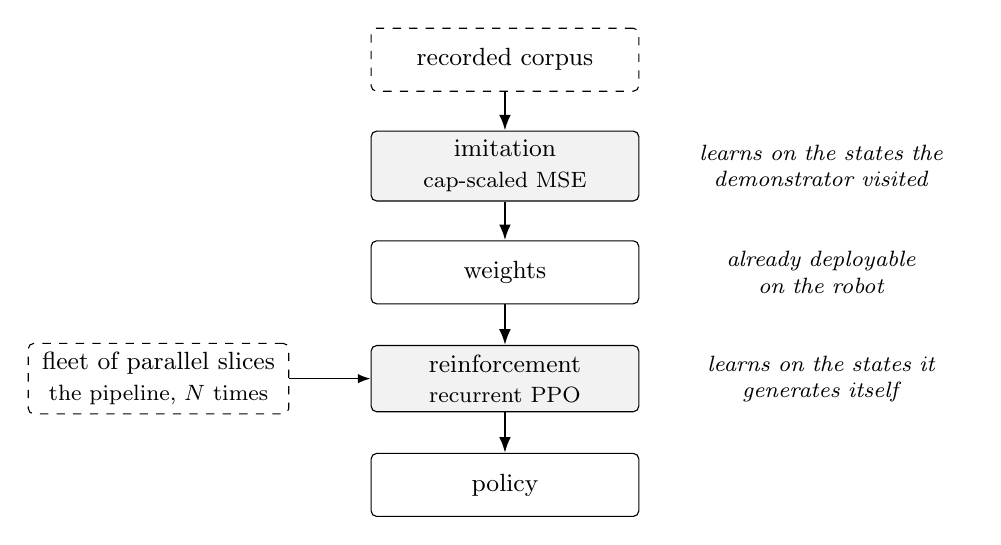
\begin{tikzpicture}[x=1cm, y=1cm, blk/.append style={minimum width=34mm}]
    \node[ext, minimum width=34mm] (corpus) at (0,0)    {recorded corpus};
    \node[lyr, minimum width=34mm] (sup)    at (0,-1.35) {imitation\\\footnotesize cap-scaled MSE};
    \node[blk] (w)      at (0,-2.70) {weights};
    \node[lyr, minimum width=34mm] (rl)     at (0,-4.05) {reinforcement\\\footnotesize recurrent PPO};
    \node[blk] (pol)    at (0,-5.40) {policy};

    \draw[flow] (corpus) -- (sup);
    \draw[flow] (sup) -- (w);
    \draw[flow] (w) -- (rl);
    \draw[flow] (rl) -- (pol);

    \node[ext, minimum width=30mm] (fleet) at (-4.4,-4.05)
      {fleet of parallel slices\\\footnotesize the pipeline, $N$ times};
    \draw[thin flow] (fleet) -- (rl);

    \node[note, anchor=west, text width=36mm] at (2.1,-1.35)
      {learns on the states the\\demonstrator visited};
    \node[note, anchor=west, text width=36mm] at (2.1,-2.70)
      {already deployable\\on the robot};
    \node[note, anchor=west, text width=36mm] at (2.1,-4.05)
      {learns on the states it\\generates itself};
  \end{tikzpicture}
  \caption{The two stages of Section~\ref{sec:training-strategy}. The first
           produces both the weights deployed on the robot and the starting
           point of the second; the second fine-tunes them on the distribution the
           policy itself generates, which is where the behaviour the local map
           should determine finally has a consequence.}
  \label{fig:two-stage}
\end{figure}

The policy described in Chapter~\ref{ch:lnn} is trained twice
(Figure~\ref{fig:two-stage}), and the two stages answer two limitations that
compensate for one another.

Imitation learns, from recorded routes, the command the pilot gave from the
observation the robot had. It is inexpensive --- the data already exist,
produced by the pipeline during normal use of the system --- and yields a
sensible starting behaviour. It carries, however, the structural defect recalled
in Section~\ref{sec:rel-imitation-rl}: the policy is evaluated on the
distribution of the states the demonstrator visited, whereas in execution it
visits those produced by its own actions. The defect is aggravated by the nature
of the demonstration: the pilot, human or automatic, plans its route on the true
geometry of the world, so that its command depends on the local map only
indirectly. Imitation teaches the reproduction of a behaviour, not the reaction
to what is observed.

Reinforcement learning does not have that defect, since it learns on the
distribution it generates itself and judges actions by the consequences they
produce. It requires, however, a number of interactions a real robot cannot
provide, each of which may destroy the vehicle. It is therefore carried out in
simulation, on a fleet of parallel environments.

The strategy adopted is the composition of the two: the first stage produces the
weights the robot flies with and the starting point of the second; the second
fine-tunes them on the correct distribution, where the behaviour the local map
ought to determine --- avoiding an obstacle --- finally has a consequence.

\paragraph{What the two stages share.}
The two procedures are implemented separately and share exactly three things:
the architecture table of Section~\ref{sec:module-implementation}, the way a
point cloud is packed for the encoder, and the thermal guard that suspends
training when the temperature of the machine exceeds a threshold. The sharing is
deliberately minimal and deliberately no greater: how the weights were fed is
part of what the weights mean, and two implementations of the same packing would
diverge without raising any error.

Both stages are moreover validated on simpler tasks before being applied to the
problem --- a synthetic task for the first, a standard control environment for
the second --- according to the protocol described in
Section~\ref{sec:exp-protocol}.

\section{Supervised Stage}
\label{sec:training-supervised}

\subsection{Corpus Acquisition and Recording Protocol}
\label{sec:sl-corpus}

The corpus is recorded through the pipeline itself, by the node described in
Section~\ref{sec:observation-recording}: every sample pairs the observation
available to the vehicle with the command that followed from it. A property no
other arrangement could guarantee follows from this: the distribution on which
the network is trained is produced by the same code that will feed it on board.

One episode corresponds to one directory. A mission may record a flight whole or
in two segments --- the outward and the return leg --- each of which becomes an
episode of its own while sharing with the other the world, the starting position
and the goal. It is a circumstance the data split must be aware of, and
Section~\ref{sec:sl-split} returns to it.

Every episode carries a metadata file describing it: the robot, the world, the
voxel pitch, the list of the archives that compose it, and a statistical summary
of the recorded commands. The summary is accumulated \emph{while} writing rather
than derived afterwards, because deriving it afterwards would mean reopening
every archive of the corpus: an operation of seconds over ten gigabytes and
impracticable over a terabyte, which would moreover have to be repeated at every
change of seed.

\subsection{Dataset Format: Sharded Episodes and Manifest}
\label{sec:sl-dataset}

Episodes are stored as sequential archives, read as a stream rather than loaded
into memory. The format imposes a property that conditions the structure of the
sample: since the archives are read in shuffled order, every sample must stand
on its own. The state block is therefore repeated in each sample although it is
constant within a recording --- a few dozen bytes against the tens of kilobytes
occupied by the voxels --- rather than being stored once per episode.

Building the \emph{manifest} of the corpus, that is the list of the episodes
with their properties, reads the metadata files exclusively and never opens an
archive. It is this separation that makes it possible to recompute a data split
in negligible time.

\subsection{Stratified Split and Episode Balancing}
\label{sec:sl-split}

Splitting per \emph{sample} would produce a meaningless evaluation: adjacent
frames of the same flight are nearly identical, and putting some of them in
training and the others in validation means measuring training and calling it
validation.

Splitting per \emph{episode} repeats the same error one level higher, for the
reason set out in Section~\ref{sec:sl-corpus}: the two segments of a flight
recorded in two parts share world, start and goal, and would end up on opposite
sides of the split. The unit adopted is therefore the \emph{run}, declared in
the metadata, of which a flight recorded whole is the particular case with a
single segment.

Runs are moreover stratified on what changes the distribution of the data: the
robot model, since different platforms command different things; the world,
since the statistics of the obstacles change; the voxel pitch, since the
quantisation changes and with it the extent of the grid
(Section~\ref{sec:observation-cloud}); and the set of command components the
episode actually exercises, since an episode in which the robot never turns
teaches nothing about turning.

Two provisions complete the protocol. The split is governed by a seed of its
own, distinct from the one that initialises the weights and the shuffling:
repeating a session under a different seed therefore measures what that session
is worth and not what a different split is worth. And the test partition is read
once, at the end, since consulting it between sessions would turn it into a
second validation partition.

\subsection{Sequence Chunking and Hidden-State Propagation}
\label{sec:sl-sequences}

A recurrent network is trained on windows of consecutive samples. The length of
the window fixes the horizon over which the gradient propagates backwards; the
step between the start of one window and the start of the next determines
instead how many windows are obtained from the same recordings, and a step
shorter than the length makes them overlap, which is the cheapest answer
available to a small corpus.

A window is cut wherever the interval between two samples exceeds a threshold: a
sequence that straddles a prolonged silence is not a sequence. The first step of
every window is moreover given the median interval of the window itself rather
than a null value, because a null interval pins the gate of the CfC cell at
exactly $0.5$ --- the degeneration discussed in Section~\ref{sec:cell-cfc} ---
precisely at the step where the state has just been cleared.

The recurrent state is governed by the mechanism of
Section~\ref{sec:module-implementation}: cleared before every window, because
each is an independent sample of the distribution of trajectories and carrying
into it the memory of the previous one would mean training on a history the
sample does not have; and detached from the graph after every optimiser step,
because otherwise the graph would grow from one mini-batch to the next until it
covered the whole epoch.

\paragraph{The composition of the batch.}
The sparse convolutional operator accepts a single grid shape per call, so that
a batch may contain only samples of the same grid. The most immediate
realisation --- one episode per batch --- satisfies the constraint but imposes a
stronger one than necessary: with overlapping windows a batch then holds few
distinct scenes, all of the same recording, and the encoder has nothing to
contrast within it. The loader therefore keeps several archives open at once and
fills one pending batch per grid drawing from all of them, so that the effective
constraint is the grid and not the episode. Validation and test keep one episode
per batch regardless, so that their figures remain comparable across sessions.

\subsection{Data Augmentation}
\label{sec:sl-augmentation}

The only transformation applied to the data is the left--right reflection of a
training window, through the longitudinal plane of the body, before it is
batched. The reflected flight is as valid as the recorded one for a vehicle
symmetric about its own longitudinal axis, and it doubles the scenes the encoder
observes on each side.

The reflection is correct only if applied to \emph{everything} that has a side,
and this is the delicate point of the transformation: the lateral index of the
cloud about the centre of the grid, the lateral component of the pose, of the
goal and of the centre of mass, the lateral velocity and command, and the axial
quantities --- the roll and yaw rates, and the corresponding components of both
quaternions. The targets of the auxiliary supervision of
Section~\ref{sec:sl-geometry} swap sector $k$ for sector $-k$. A window is
reflected whole and never step by step, and validation never is.

\subsection{Observation Normaliser Fitting}
\label{sec:sl-normaliser}

The affine transform described in Section~\ref{sec:aux-modules} is estimated
from the data before training, over a bounded number of batches, and stored
inside the weights. It follows that inference on board applies it without
knowing: there is no normalisation step external to the network that a node
might forget to perform.

Features of zero variance require explicit treatment. Since the normalisation
divides by the standard deviation bounded below by a minimum value, a feature
constant over the corpus would be divided by that minimum, and the day it ceased
to be constant --- a tilted goal, a limit changed in the configuration --- it
would enter the network amplified by six orders of magnitude. The deviation of
such features is therefore raised to one. The correction is neutral on constant
data, since a deviation from the mean that is identically zero remains zero
whatever the divisor.

\subsection{Cap-Scaled Mean Squared Error Loss}
\label{sec:sl-loss}

The mean squared error computed on the raw command is dominated by the component
that carries the most energy, and the six components of a velocity command
differ from one another by orders of magnitude in variance: the gradient
reaching the small ones is negligible, and they are in effect never learnt.

The customary correction --- dividing by the per-dimension standard deviation
measured on the corpus --- is not applicable here, for two reasons. Some
components are identically zero over the whole corpus, so their scale would be
an arbitrary value of convenience. And every scale would shift as new recordings
arrived, silently reweighting the loss function between sessions meant to be
comparable.

The loss adopted divides instead by the \emph{velocity limits declared by the
robot}, which are already present in the state block of the observation
(Section~\ref{sec:observation-vector}); its formal definition is given in
Section~\ref{sec:metrics-loss}. Three properties follow. The error becomes a
fraction of what that robot can do, so that platforms with very different limits
are directly comparable. The scale is a property of the platform and not of the
corpus, and does not move when data is added. And a heterogeneous fleet requires
no special case, since every sample carries its own limits.

\subsection{Auxiliary Geometry Supervision}
\label{sec:sl-geometry}

For the reason set out in Section~\ref{sec:geometry-head}, imitation alone
provides the encoder with a weak signal. The auxiliary supervision adds a second
objective that requires no labels.

The targets are measured once per corpus, before training, on the cloud of each
frame: the distance to the nearest obstacle in each of eight azimuth sectors and
the height above the ground. The measurement is performed with the same
functions the perception bridge uses on board --- the same estimate of the
ground and the same exclusions of the hull of the vehicle --- so that the
encoder is taught exactly the quantity the reward of the reinforcement stage
prices (Section~\ref{sec:rl-reward}). The result is written beside each episode.

The overall loss is the sum of the imitation loss and the auxiliary one,
weighted by a coefficient. Two properties of the protocol must be stated because
they make sessions with and without the auxiliary term comparable. The first is
that the losses recorded as training and validation loss remain the imitation
loss alone, so that two sessions are ranked on the same quantity. The second is
that the output of the encoder is computed once per batch and handed to the
network, rather than being recomputed for the auxiliary head: the sparse
convolution, which is the expensive part of the forward pass, is not performed
twice.

\subsection{Optimisation and Checkpoint Selection}
\label{sec:sl-optimisation}

The optimiser is AdamW, with a weight penalty sized as a regulariser rather than
as a constraint. The learning rate decays linearly towards a fraction of its
initial value rather than towards zero, so that the last epochs keep learning
instead of merely not getting worse; the gradient norm is clipped at every step.

The horizon of the decay requires knowing the number of steps per epoch, which a
streaming loader does not declare: it is supplied as an initial estimate and
measured for real on the first pass, after which the schedule is retargeted onto
the observed value.

\textbf{No automatic early stopping is provided.} Every epoch produces a
checkpoint, and the epoch that minimises the validation loss is flagged:
selecting the checkpoint is part of the experimental protocol
(Section~\ref{sec:exp-protocol}) and not a decision taken by the training. The
choice is deliberate --- stopping automatically would mean fixing the criterion
once and for all, whereas the criterion is what Chapter~\ref{ch:results} must be
able to discuss. A checkpoint may accordingly be reloaded in two ways: with its
weights alone, which is what starting a new session from them requires and is
the case of the reinforcement stage, or in full, which also restores the state
of the optimiser and the position in the schedule and is what continuing an
interrupted session requires.

Two seeds govern reproducibility: one initialises the weights and the shuffling,
the other the data split alone (Section~\ref{sec:sl-split}). A thermal guard,
finally, suspends training when the temperature of the machine exceeds a
threshold and resumes it only once it has fallen by a margin, so that a machine
at the limit does not alternate suspension and resumption at every check.

\subsection{Output Calibration Fitting}
\label{sec:sl-calibration}

The recalibration of the output, motivated in
Section~\ref{sec:output-calibration}, is estimated according to a precise
protocol, which belongs to this chapter while its purpose belongs to the
previous one.

Validation is run with the calibration stage at the identity, and the
calibration is estimated \emph{from those same predictions}, afterwards. The
ordering is not arbitrary: a model is already calibrated with respect to the
data on which it was optimised, so that an estimate made on the training set
would read a gain close to one and would under-correct everywhere else.

The estimate is repeated at every epoch, so that each checkpoint carries the
calibration belonging to its own weights. A gain exceeding a declared maximum is
clipped and reported: if the spread of the prediction is a small fraction of
that of the command, the least-squares line is extrapolating.

\section{Reinforcement Stage}
\label{sec:training-rl}

\subsection{Problem Formulation}
\label{sec:rl-pomdp}

The task is formulated as a partially observable Markov decision process, and it
is worth identifying its components on the concrete problem rather than in the
abstract.

The \emph{state} comprises the configuration of the vehicle --- pose, velocity,
attitude --- and that of the environment surrounding it; the agent never has
access to it. What it receives is the \emph{observation} defined in
Section~\ref{sec:observation-space}, produced by the same pipeline that produces
it on board, and which is a partial and noisy function of that state. The
\emph{action} is the six-component velocity command, continuous and expressed in
the physical units of the platform. The \emph{transition} is determined by the
dynamics of the simulated vehicle and by the latency of the chain that produces
the observation: between the measurement on which the agent decides and the
effect of the command lies the traversal time of the pipeline, which is part of
the problem rather than a defect to be compensated for. The \emph{reward} is
discussed in Section~\ref{sec:rl-reward}, the episode horizon in
Section~\ref{sec:rl-episodes} and the discount factor in
Section~\ref{sec:rl-presets}.

\paragraph{What the partial observability consists of.}
It is not a formality: on this problem it has three distinct origins, and all
three have consequences for the learnt behaviour. The local map represents what
the sensors have observed and not yet forgotten
(Section~\ref{sec:observation-map}), so that a region never framed is
indistinguishable from a free one. The pose is an estimate subject to drift
rather than the true position, and the goal is expressed relative to it. A single
frame, finally, says nothing about what was happening: whether the vehicle was
accelerating, whether the obstacle ahead is approaching or receding, how long it
has been standing still.

\paragraph{The policy is a function of the history.}
It follows that, in principle, the optimal policy is a function not of the last
observation but of the sequence preceding it; how much of that history a policy
actually needs on a given task is an empirical question, which the stateless
control answers in Chapter~\ref{ch:results}. The two customary treatments are to stack a window
of observations into a single vector, or to maintain a state updated at every
step; the architecture of Chapter~\ref{ch:lnn} adopts the second, so that the
policy is $\pi_\theta(a_t \mid o_t, x_t)$, with $x_t$ the recurrent state
summarising the history. It is this choice that makes a recurrent version of the
algorithm necessary, and Section~\ref{sec:rl-buffer} describes its consequences.

\paragraph{The steps are not equally spaced in time.}
The formulation assumes that a step is a decision, but the duration of a step is
not constant: it depends on the rate at which the pipeline delivers the
observation (Section~\ref{sec:observation-recording}). The interval actually
elapsed is therefore part of what the policy reads, and it is the quantity with
which the cell integrates its own dynamics (Section~\ref{sec:cell-time}). The
same quantity is used by the environment to size the episode, which is defined
in steps but measured over a time (Section~\ref{sec:rl-episodes}).

\paragraph{The platform is not part of the hidden state.}
A last property distinguishes this formulation from the customary one of a
learnt navigation task, and it is the reason why a single policy can be trained
on a heterogeneous fleet. The identity of the body is not a latent variable the
agent must infer from the behaviour of the vehicle: it is declared in the
observation, in the kinematic limits and in the model identifier of
Section~\ref{sec:observation-vector}. Changing platform is therefore a change of
observation and not of problem --- the action space, the reward function and the
objective remain the same --- and it is what allows the experience of different
robots to be gathered into a single training.

\paragraph{The objective.}
The policy maximises the expected discounted return over the episodes generated
by the fleet. During training it is stochastic, since exploration is obtained by
sampling from a distribution whose width is itself trained
(Section~\ref{sec:rl-actions}); that width, however, belongs to the algorithm
and not to the network, so that the policy transferred on board is the mean of
that distribution, that is deterministic.

\subsection{Recurrent PPO: Objective and Clipping}
\label{sec:rppo-gae}

Policy-gradient methods improve the policy by raising the probability of the
actions that turned out better than expected. In the naive form this is valid
only for the data collected by the current policy: every batch can be used
exactly once, and a step too large destroys the policy without there being a
loss function to fall back on.

Proximal policy optimisation \cite{schulman2017ppo} buys reuse and safety by
keeping the updated policy \emph{close} to the one that collected the data.
Closeness is measured by the probability ratio of the action actually taken,
\begin{equation}
  r_t(\theta) = \frac{\pi_\theta(a_t \mid s_t)}{\pi_{\theta_{\text{old}}}(a_t \mid s_t)},
  \label{eq:ppo-ratio}
\end{equation}
and the objective is clipped so that drifting beyond a threshold ceases to be
profitable:
\begin{equation}
  L_{\text{policy}} = -\,\mathbb{E}\!\left[\min\!\left(r_t A_t,\;
     \operatorname{clip}(r_t, 1-\epsilon, 1+\epsilon)\, A_t\right)\right].
  \label{eq:ppo-clip}
\end{equation}

Equation~\eqref{eq:ppo-clip} reads as a hinge. If an action turned out better
than expected, raising its probability improves the objective until the ratio
reaches $1+\epsilon$, beyond which the clipped branch takes over and the
gradient vanishes: the update stops of its own accord. Symmetrically for an
action worse than expected.

An entropy bonus is subtracted from the objective, preventing the policy from
collapsing prematurely onto a single action. The critic is trained by regression
onto the returns, with the option of clipping its update as well with respect to
the value predicted during collection, so that a single mini-batch does not
rewrite the value function. Actor and critic have separate optimisers and
separate backward passes, and each receives its own clipping of the gradient
norm.

\subsection{Generalised Advantage Estimation and Truncation Bootstrapping}
\label{sec:rl-gae}

The advantage $A_t$ could be estimated as the difference between return and
value, but the return is a sum of many noisy rewards, while the one-step
estimate is biased by the critic's error. Generalised advantage estimation
\cite{schulman2016gae} interpolates between the two:
\begin{align}
  \delta_t &= r_t + \gamma\, V(s_{t+1})\,(1 - d_t) - V(s_t), \\
  A_t      &= \delta_t + \gamma\,\lambda\,(1 - d_t)\, A_{t+1},
  \label{eq:gae}
\end{align}
computed backwards over the rollout, where $d_t$ marks the end of an episode and
the factor $(1-d_t)$ prevents the trace from crossing its boundary.

\paragraph{Truncation and termination are not the same thing.}
An episode that has reached the time limit is not finished: the state in which
it stopped has a value, and treating it as zero introduces a systematic bias in
the critic precisely where episodes almost always end. The reward of a truncated
step therefore receives, during collection, the addition of $\gamma\,V$ computed
on the final observation --- which at that moment still exists, whereas the
automatic reset has already replaced it in the one returned. The advantage
estimate then uses the end-of-episode signal for both cases and does not repeat
the addition, which would count the value twice. An environment that truncates
without providing the final observation raises an error rather than silently
reintroducing the bias.

\subsection{Recurrent Rollout Buffer and Sequence Replay}
\label{sec:rl-buffer}

That the network carries memory between observations --- which is the reason it
was chosen --- has consequences for the organisation of the collected data and
for the update, and it is what distinguishes this realisation from a stateless
implementation.

\paragraph{The unit of a mini-batch is a sequence, not a sample.}
A mini-batch counts sequences of consecutive steps of a single environment; only
the stateless path shuffles individual samples. The buffer stores, for every
step and besides the transition, the snapshot of the recurrent state taken
\emph{before} the forward pass, since it is the state that produced that action.

\paragraph{Backpropagation is truncated at the window.}
The update replays every sequence forwards, one step at a time, feeding the
network its own output state as the next input: the gradient flows through the
length of the window and no further. The initial condition is the snapshot
stored at the start of the window.

\paragraph{The stored action is the sampled one.}
The environment clips the command within the limits declared by the platform
before applying it, but the buffer keeps the action as the policy sampled it.
The stored log-probability must remain that of \emph{that} action, or the ratio
of Equation~\eqref{eq:ppo-ratio} would be a ratio between two different
quantities.

\paragraph{What is not real must not contribute.}
The last window of a rollout is usually shorter than the nominal length, and
every loss is therefore masked and divided by the number of real positions
rather than by the size of the tensor. Likewise, an episode boundary inside a
window clears the state of the columns that ended and of those alone, so that
the memory of one episode does not leak into the next. The batch, finally, is
never split across environments: the cells hold every environment's state
together, and splitting it would fragment that state.

\subsection{Actor, Critic and Shared Encoder}
\label{sec:rl-networks}

The actor is one of the networks of Chapter~\ref{ch:lnn}, built from the same
table the supervised training uses: there is no separate actor hierarchy, since
the base class of the networks already provides the handling of the recurrent
state on which the algorithm relies.

The critic is instead a network of its own and deliberately distinct from the
actor. On an environment that includes the point cloud it also receives the
descriptor of the encoder, concatenated with the dense observation: a value
function that cannot see the obstacles is estimating a different problem from
the one the policy is solving.

One point deserves attention because violating it produces numbers rather than
errors. The critic reads the observation \emph{through the actor's
normalisation} --- a view onto the latter's statistics, neither a second
normaliser nor a copy of those statistics. With a pretrained network, which
carries its own normalisation inside the weights
(Section~\ref{sec:rl-finetuning}), a critic reading the raw vector would receive
quantities orders of magnitude out of scale --- among them the model identifier
--- and would saturate at the first nonlinearity, reducing itself to predicting
a constant. The view is not registered as a submodule, so that the statistics
exist once only and a later load onto the actor cannot leave the two in
disagreement, and it takes the leading components of the observation, since the
fixed-step variants append the elapsed interval to it
(Section~\ref{sec:cell-time}).

\paragraph{The encoder: frozen or trained.}
The sparse encoder may be kept fixed or fine-tuned along with the rest. Freezing it
allows the descriptor rather than the cloud to be stored in the buffer, and the
convolution not to be run during the update. Training it costs an additional
convolution over every sample of every epoch, and the memory to hold its graph,
which is proportional to the product of sequence length and batch size and to
the volume of the grid rather than to the number of occupied voxels.

The choice is not free in one case, however: starting from random weights, a
frozen encoder produces nearly identical descriptors for any cloud, so that the
policy would fly on odometry alone and no amount of steps would correct it.
Starting from scratch and training the encoder are therefore a single choice,
and their contrary combination is refused rather than executed.

\subsection{Action Distribution and Bound Penalty}
\label{sec:rl-actions}

The action space is continuous and the policy is Gaussian: the network produces
the mean, while the spread is a trained parameter that lives on the \emph{agent}
and not on the network. The placement is motivated: without it there would be no
sampling, no log-probability, no ratio and no entropy --- it is part of the
algorithm and not of the architecture, and a network exported to the robot need
not carry it.

The spread is initialised at a fraction of the action envelope declared by the
environment, and not at a fixed value: a unit standard deviation would be wider
than the entire action space on a platform with tight limits, and on a
pretrained network it would drown the imitated policy from the first step.

A penalty term finally charges the part of the Gaussian mean that falls outside
the envelope. Without it the network may push the mean arbitrarily beyond the
limit, since the environment clips the command in any case: the policy would pay
in entropy and in exploration for a region of the action space it cannot reach.

\subsection{Vectorised Fleet Environment and Domain Randomisation}
\label{sec:rl-environment}

The environment is not a simulator but a \emph{fleet} of isolated copies of the
entire system. Each parallel environment --- a \emph{slice} --- is a complete
vertical stack: the simulator with its own world, the bridge towards the ROS
channels, and a reduced version of the pipeline of
Chapter~\ref{ch:pipeline}. Isolation between slices is obtained on three
distinct planes --- middleware domain, simulator partition, communication port
--- and the training attaches to them through one socket per slice. A property
important to the interpretation of the results follows: the observation on which
the policy is fine-tuned is produced by the same chain that produces it on board,
and not by a simplified model of the environment.

The fleet is moreover the way domain randomisation reaches this network. What
must necessarily agree across slices is whatever sizes the actor and the buffer:
the width of the dense observation, the presence of the cloud, the width of the
action, and the names of the signals the reward is built from. What must
\emph{not} agree is everything else --- the extent and the resolution of the
grid, the robot model, the goal, the kinematic limits --- and it is precisely of
those differences that the randomisation consists. The circumstance is so
structural that the voxel pitch is one of the components of the dense
observation (Section~\ref{sec:observation-vector}): the network is not required
to infer the resolution it is looking at, it is told.

The effective heterogeneity is, however, a property of the fleet manifest and
not of the code: slices are assigned cyclically to the available configurations,
and a manifest built from a single configuration produces identical slices
without anything downstream complaining. It is a condition the experimental
protocol must verify before a long session rather than infer afterwards.

\subsection{Episode Policy: Spawn, Termination and Truncation}
\label{sec:rl-episodes}

What an episode on a slice is, is decided by the environment and not by the
training, and it is entirely \emph{derived from what that slice declares}: the
maximum number of steps from the ratio between the distance of the goal and the
envelope speed, multiplied by a budget factor; the arrival tolerance as a
multiple of the voxel pitch of that slice, so that the threshold remains
commensurate with the resolution at which that slice measures; the tipping angle
as pure geometry; the seed from the slice's own episode counter.

\paragraph{The budget factor is a demand on speed.}
Since the maximum number of steps is sized on the envelope speed, allowing a
multiple of the ideal time is the same as demanding an average speed equal to
the envelope divided by that multiple. It is a claim about the policy and not
about the world, and it is to be checked against the speed the policy actually
holds: a budget the demonstrator itself would not meet cannot be met by a policy
fine-tuned from it, and it makes arrival structurally unreachable.

\paragraph{Every episode restarts from the spawn.}
An episode resuming half way along the route would be a shorter task scored on
the same scale, and the return would report an improvement where the vehicle had
merely been asked to do less. Restarting from the origin moreover preserves the
meaning of the deadline, which measures the trip from the start, and prevents a
robot stuck against an obstacle from being truncated in place indefinitely,
which would make the distribution of the initial states a function of the
policy's own failures.

\paragraph{The task belongs to the slice.}
This is a distinct question from the previous one. The spawn and the goal are
part of the configuration of each slice, like its robot and its world, and are
not drawn by the training: every slice poses the same trip at every episode.
What varies is the trip from one slice to the next, so that a fleet can pose
tasks of graded difficulty side by side --- short trips with the goal in view
next to longer ones with obstacles on the straight route --- and every batch of
data then holds them in fixed proportions. This is not a curriculum: no task
follows another, and the training does not know which slice is easy. The
fleet used in the experiments is described in Section~\ref{sec:res-rl-fleet}.

\paragraph{The terminal conditions.}
An episode ends on arrival within the tolerance, on tipping beyond the declared
angle, on contact when a collision margin is armed, or on stalling. The last
condition deserves a motivation, because it is not a geometric threshold: the
distance from obstacles is measured from the centre of the vehicle, and is
therefore in fact a threshold on the sphere enclosing its body --- an acceptable
model for a multirotor and an inadequate one for an elongated ground vehicle,
whose sphere is inside a wall whenever it merely drives past one. The
consequence of contact, however, requires no geometry: a robot commanded forward
that does not move forward has hit something. Stalling ends the episode after a
number of consecutive steps below a fraction of the commanded speed, and only
when the command exceeds a minimum threshold --- standing still is a legitimate
thing to be told to do. It is armed per slice and only where it separates the
two cases, that is on the platforms that do not fly.

Reaching the step limit finally produces a \emph{truncation}, which the
algorithm treats differently from a termination (Section~\ref{sec:rl-gae}).

\subsection{Reward Design}
\label{sec:rl-reward}

The reward is not fixed: it is a policy chosen among several, and its structure
is a list of cost terms plus a single term that earns. Every term knows its own
name, its share of the budget and its own arithmetic, and is logged separately,
so that the contribution of each is readable.

\paragraph{The term that earns.}
Progress towards the goal is formulated as potential-based shaping
\cite{ng1999policy}, with potential equal to the negative of the distance to the
goal. The canonical form, $d_{\text{prev}} - \gamma d$, is invariant with
respect to the optimal policy, but it pays $(1-\gamma)d$ to a stationary vehicle
--- \emph{the more so the further away it is}. If the discount factor is derived
from the episode length, as described in Section~\ref{sec:rl-presets}, that rate
works out at exactly the ceiling below which the dense costs must be held: no
allocation of the shares can then make loitering unprofitable, since the matter
is excluded by construction and not by tuning. The policy adopted therefore pins
at one the discount of the shaping term alone, which thus pays the metres
actually closed. What is given up is exact invariance under a discounted return;
what is obtained is that same invariant form minus a cost proportional to the
distance still to go --- loitering far costs more than loitering close, which is
a term one would write on purpose.

\paragraph{The barriers.}
Three of the ways the vehicle is lost --- contact, tipping over, leaving the
altitude band --- have the same shape: a quantity approaching a threshold past
which the episode ends. They therefore share a single term, quadratic, null up
to a soft threshold and clipped at one beyond the hard one. Each of the three
choices answers a failure of the obvious alternative. Without the soft threshold
the cost would jump from nothing to the terminal penalty, leaving no gradient
along which to learn not to arrive there. A linear ramp would tax the useful
manoeuvre as much as the dangerous one --- a multirotor tilts in order to
accelerate and passes close to a wall in order to get past it --- whereas the
quadratic leaves the useful zone almost free. And an unbounded barrier would
dominate every other term as soon as the violation is large, and would have no
finite worst case, so that neither of the two budget constraints below could be
verified at all.

The safety barrier, in particular, is measured not against a constant distance
but against the room needed to stop,
\begin{equation}
  d_{\text{safe}}(v) = d_0 + \tau v + \frac{v^2}{2 a_{\text{brake}}},
  \label{eq:stopping}
\end{equation}
where $d_0$ is the radius of the sphere enclosing the vehicle plus a standoff,
and $\tau$ is the latency of perception and actuation. The altitude barrier is
defined around a cruise altitude and expressed as a fraction of it, so that it
follows the vehicle rather than the map, and it leaves out of the term the
slices to which no vertical velocity is sent.

\paragraph{The terminals, and the scale of everything else.}
A terminal term assigns the arrival bonus --- reduced in proportion to the speed
at which the goal is reached, since arriving into the goal is not arriving ---
and the penalty for losing the vehicle. Every other magnitude is expressed as a
fraction of what the slice declares: the maximum progress for the costs, the
terminal angle for the attitude ramp, the action envelope for the command
smoothness term, the map radius for the altitude band. A faster robot, a
different step or another simulator move all of them without anyone having to
remember to.

\paragraph{The two budget constraints.}
The shares must satisfy two inequalities. Per step, their sum must be below one:
above that, the best available policy is to stop paying, by standing still or by
ending the episode at once. Per episode, the sum must be below the reciprocal of
the budget factor, since a slow success over $k$ times the ideal time pays $k$
times the costs while earning the same distance; requiring the inequality to
hold for any distance yields $\sum f < 1/k$. It is a design rule rather than a
number to be retuned for every goal, and it is verified at the construction of
the policy and at the connection to the fleet, where the length of the episodes
is known.

\paragraph{The budget is necessary and not sufficient.}
Satisfying it guarantees that no allocation of the shares pays for ending an
episode early. It says nothing about how much the terms, \emph{together}, pay
for flying rather than for standing still, and a configuration may respect the
ceiling and converge to immobility all the same, because what the constraint
cannot see is the relative magnitude between the channels. A reward
configuration is therefore \emph{priced before} the session, at the operating
points at which the fleet has been measured, answering the two questions that
decide a session before it begins: whether flying pays better than creeping, and
above what probability of arriving trying pays better than not trying.

\subsection{Observation and Reward Normalisers}
\label{sec:rl-normalisers}

The agent has three optional normalisers --- of the observation, of the reward
and of the returns --- and a fourth constraint which is not optional and has no
switch, namely that the critic read the observation through whatever reads it
for the actor (Section~\ref{sec:rl-networks}).

The observation normaliser \emph{must stay off} with a pretrained network, which
carries its own normalisation inside the weights: a second normalisation on top
would feed it an input it has never seen. The combination is refused rather than
executed. The reward normaliser divides by the running standard deviation of the
discounted return and does \emph{not} subtract its mean, since subtracting it
would change the sign of the reward.

Two properties of the recursive estimation of the statistics deserve to be
stated, because both arise from characteristics of this observation. The first
is that the estimate accumulates the sum of squared deviations and not the
variance: the two coincide only as long as every column varies, whereas in this
observation a substantial part of the columns is constant by construction ---
the goal block, the declared envelope of the robot, the model identifier --- and
carrying a variance would mean treating as a measurement the value of
convenience assigned to a constant column, then diluting it at every batch. The
second is that every sample is bounded to a number of deviations before being
folded in: there being no forgetting factor, a single reading coming from a
diverged estimator would become, for good, the scale by which everything else is
divided.

\subsection{Trust Region, Entropy and Schedules}
\label{sec:rl-schedules}

After every mini-batch the approximate divergence between the policy that
collected the data and the current one is measured, with the low-variance
estimator $\mathbb{E}[(r-1) - \log r]$. When the running mean of the epoch
exceeds a threshold, the actor stops for the rest of the update: the data no
longer describe the current policy, and the following epochs would optimise with
respect to a distribution that has moved. The critic continues, having no ratio
and nothing to be wrong about.

\paragraph{The mean, and not the sample that produced it.}
The criterion is read on the mean and not on the individual mini-batch, and this
is a substantive choice. A mini-batch is here the product of sequence length and
batch size, and on so few samples the estimator is heavy-tailed: stopping at the
first sample beyond the threshold means stopping at the maximum of many noisy
draws, which exceeds any threshold close to the mean. The region is therefore
not consulted until a minimum number of informative estimates is available,
since the standard error falls as the square root of their number. Moreover,
only the mini-batches scored \emph{after} the policy has moved enter that mean:
until the first optimiser step the weights are still the ones that collected the
rollout, the ratio is exactly one and the estimate exactly zero, and including
them would lower the mean by an amount that depends on the size of the gradient
buffer rather than on the policy.

\paragraph{The schedules.}
The learning rate and the clipping width $\epsilon$ both decay linearly towards
a fraction of their initial value rather than towards zero: early on, large and
exploratory steps are wanted; late on, a policy that settles. The horizon of the
decay is derived from the step budget, so that raising it does not merely
lengthen the session but also re-paces its schedule.

\paragraph{One knob wearing four names.}
The initial exploration width, the actor's learning rate, the trust-region
threshold and the number of mini-batches accumulated per step are not
independent parameters. The divergence grows as $\Delta\mu^2/2\sigma^2$ and the
gradient on the mean as $A(a-\mu)/\sigma^2$: the trust region is therefore
\emph{measured in units of the exploration width}, and narrowing the latter
makes the same policy step far larger in the eyes of the stopping criterion.
They must therefore be tuned together, which is why they are the only parameters
of the algorithm the command line exposes beside those of the environment.

\subsection{Fine-Tuning from Imitated Weights}
\label{sec:rl-finetuning}

Loading an imitation checkpoint rebuilds the network from the declaration held
in the metadata, by the same route the inference node takes on board: training
and inference load the same file in the same way. Three adjustments are applied
on the way in, and each of them guards against a failure that would produce
numbers rather than an exception.

\begin{enumerate}
  \item \textbf{The external normalisation stays off}, for the reason given in
        Section~\ref{sec:rl-normalisers}.
  \item \textbf{Degenerate statistics are repaired}, as in
        Section~\ref{sec:sl-normaliser}. The repair is neutral on constant data,
        and fine-tuning is precisely what makes those features start to vary.
  \item \textbf{The output calibration becomes trainable.} Kept fixed, a
        component the demonstration never exercised has zero correlation, hence
        zero gain: under fine-tuning that factor multiplies the gradient too, so
        that the component is not attenuated but \emph{disconnected} --- and
        those are exactly the components pretraining got wrong. The trainable
        mode starts from the estimated values and lets them move.
\end{enumerate}

\paragraph{The first iterations.}
A pretrained actor arrives with a policy worth keeping and a critic that knows
nothing. The first advantages are therefore the critic's error, and the
algorithm would spend the first iterations moving good weights with them --- the
encoder included, where it is trainable. A configurable number of initial
iterations is therefore reserved for the critic alone: while it lasts, the
actor's weights, its exploration width and the auxiliary head remain unchanged
bit for bit. The phase has moreover an experimental value of its own, and it is
stated here because Chapter~\ref{ch:results} relies on it: for its whole
duration the performance metrics describe the imitated policy exactly as
imitation left it, and constitute therefore its only free measurement on the
fleet.

\paragraph{Starting over or continuing.}
Starting from the weights alone begins a new session, with critic, optimisers
and exploration width afresh; continuing an interrupted one also restores them,
together with the statistics of the normalisers and the position in the
schedule, each of which would otherwise make the resumption read as a regression
that did not occur.

\paragraph{What can be transferred on board.}
A policy fine-tuned from imitation carries the statistics of the corpus inside its
own weights and is transferable as it stands. A policy trained from random
weights is not: its internal normalisation is the identity, and the
normalisation that made the training work lives in the agent's recursive
estimator, which inference never opens. In the second case the statistics must
be written into the network before export, an operation the dedicated tool
performs while refusing the cases in which it would be ambiguous --- a
checkpoint carrying them in both places, or in neither.

\subsection{Hyperparameter Presets}
\label{sec:rl-presets}

The hyper-parameters of the algorithm are declared as data, one set per
architecture, rather than as arguments scattered among the call sites: changing
architecture is a choice on the command line, changing a value is an edit in a
single visible place. Each set moreover provides a \emph{substitution} for
starting from random weights, which alters the few values that regime requires
to differ --- a higher learning rate and entropy bonus, a wider initial
exploration, no phase reserved for the critic, there being no policy to protect,
and the external normalisation of the observation switched on, since in that
regime the network carries none of its own inside. It is the same difference
that Section~\ref{sec:rl-finetuning} states with respect to transfer on board.
The command line reaches only the parameters on which a fleet is genuinely
retuned, and every value differing from the default set is printed at startup,
so that the session itself declares what it was started with.

\paragraph{One discount per slice.}
The discount factor deserves separate treatment, because a heterogeneous fleet
admits no single one. Resolving it as $\gamma = 1 - 1/T$ from the episode length
$T$ of each slice makes $\gamma^{T}$ equal to $1/e$ on all of them: the arrival
bonus is equally visible from every spawn. A single value derived from the mean
would instead give slices with very different trips very different horizons,
posing in effect the same task as two distinct problems, and making the bonus
nearly invisible to the longest slice. The same per-slice value is read by the
advantage trace, by the value added on truncation, by the reward normaliser and
by the progress potential, so that nothing is discounted twice with two
different values.


\part{Experiments}
Part~II describes how the work is measured and what it measured. It fixes the
infrastructure, the protocol and the two families of metrics before reporting a
single result, so that no number in the last chapter is read on a scale defined
after it was obtained.
%!TEX root = ../main.tex
\chapter{Experimental Setup and Evaluation Metrics}
\label{ch:experiments}

Both training regimes used in this work---imitation of recorded flights
(Section~\ref{sec:training-supervised}) and reinforcement learning in
simulation (Section~\ref{sec:training-rl})---produce a single headline number
that the optimiser minimises: a loss in the first case, a negative expected
return in the second. Neither number answers the question that actually
matters, which is whether the resulting network flies the robot well. A
supervised loss can fall while the network learns nothing but ``predict zero'';
an episodic return can rise while the vehicle learns to crash less rather than
to reach its target. This chapter fixes, before any result is shown, the
conditions under which the numbers of Chapter~\ref{ch:results} were produced:
the machines and the software the runs were executed on, the protocol every run
follows, and every quantity that is logged alongside the headline number, what
each one measures and why it was added. The metrics are grouped by training
regime, since the two ask different questions of the model, and each group ends
with a summary table.

Every metric named here is a column in a CSV file written during training: one
row per epoch for the supervised trainer, one row per iteration for the
reinforcement trainer. The column names are quoted verbatim in monospace, so
that a figure in Chapter~\ref{ch:results} can always be traced back to its
definition here.

The chapter is organised in two halves. The first fixes the common ground: the
notation used throughout (Section~\ref{sec:metrics-notation}), the
infrastructure the experiments run on (Section~\ref{sec:exp-tooling}) and the
protocol under which the architectures are trained, validated and compared
(Section~\ref{sec:exp-protocol}). The second defines the two families of
metrics, one per training stage: supervised in
Section~\ref{sec:metrics-supervised}, reinforcement learning in
Section~\ref{sec:metrics-rl}.

\subsection{Conventions and Notation}
\label{sec:metrics-notation}

The network's output is a velocity command
$\mathbf{y} = (v_x, v_y, v_z, \omega_x, \omega_y, \omega_z) \in \mathbb{R}^{6}$:
three linear velocities in \si{\metre\per\second} and three angular velocities
in \si{\radian\per\second}. Components are indexed $i = 0,\dots,5$ in the order
above, matching the \met{_dim_<i>} suffix of the log columns. The demonstrated
(target) command is $\mathbf{y}$ and the network's prediction is
$\hat{\mathbf{y}}$; $N$ denotes the number of samples over which an average is
taken, which in sequence mode counts every time step of every window.

Each robot in the fleet declares its own kinematic limits inside the
\texttt{state} block of the observation. The per-component \emph{velocity cap}
$c_i > 0$ is the largest magnitude the platform accepts on component $i$;
a cap of zero declares that the axis does not exist on that robot (for example
vertical velocity on a ground vehicle).

For the reinforcement learning metrics the following terms are used with their
usual meaning, defined formally in Section~\ref{sec:rppo-gae}. An
\emph{episode} is one attempt at the navigation task, from spawn to a terminal
condition or to the time limit. A \emph{rollout} is a fixed number of
environment steps collected from every parallel environment with the current
policy; an \emph{iteration} is one rollout followed by one policy update, and
a \emph{mini-batch} is a subset of the rollout the update is computed on.
$\pi_\theta(a \mid s)$ is the stochastic policy, $V(s)$ the critic's estimate of
the state value, $\gamma$ the discount factor, $A_t$ the advantage of the action
taken at step $t$ and $R_t$ the corresponding bootstrapped return.

\subsection{Infrastructure and Tooling}
\label{sec:exp-tooling}

\subsubsection{Hardware and Software Environment}

Training is carried out on a single workstation equipped with an NVIDIA RTX~5080
with \SI{16}{\gibi\byte} of video memory and \SI{32}{\gibi\byte} of system
memory, on which both the training procedures and the fleet of simulated
environments run. The memory of the accelerator is the resource that constrains
the experimental design more than any other: it is shared between the training
session and the slices of the fleet, and it determines the finest grid on which
the encoder may be refined during the reinforcement stage
(Section~\ref{sec:rl-networks}).

The software environment is the one declared by the two repositories. The
networks and the training are implemented in PyTorch with CUDA support; the
sparse convolution uses \texttt{spconv}; the corpus is read as a stream through
\texttt{webdataset}; the control environment comes from \texttt{gymnasium}. The
pipeline of Chapter~\ref{ch:pipeline} and the simulators run instead in Docker
containers, so that the version of ROS~2, of the simulator and of the perception
libraries is fixed by the image rather than by the machine running it.

\subsubsection{Simulation and the Parallel Fleet}

The reinforcement stage requires many environments in parallel, and each of them
is an isolated copy of the entire system rather than a simplified model
(Section~\ref{sec:rl-environment}). The fleet is managed by a dedicated tool
that governs its life cycle in five operations: \emph{planning}, which works out
how many slices to instantiate and with which configurations, recording every
runtime parameter in a manifest; \emph{materialisation}, which generates the
files of each slice from the manifest; \emph{start-up}, which brings up the
containers and the processes in the required order; \emph{inspection}, which
reports what is running on each slice and with which configuration; and
\emph{shutdown}.

Two properties of this tool belong to the experimental protocol rather than to
the infrastructure. The first is that start-up checks which slices are actually
producing point clouds and writes a reduced manifest of them: starting a session
on a manifest that lists a slice which is not working means losing the session a
few minutes after beginning it. The second is that the number of slices can be
derived from the machine, from a measured per-slice cost and a reserve for the
training session, which runs on the same machine and itself requires cores,
memory and accelerator memory. The number so obtained states how many slices
\emph{fit} on the machine, not how many it is worth running: beyond a certain
number the overall throughput grows less than proportionally, and the choice
made in the experiments is reported in Chapter~\ref{ch:results}.

\subsubsection{Logging and Run Artefacts}

Every session produces artefacts in two distinct places, and the separation is
deliberate: what is needed to \emph{read} a session is kept apart from what is
needed to \emph{resume} it or to transfer it to a robot.

The supervised stage writes one row per epoch to a comma-separated file,
containing every metric defined in Sections~\ref{sec:metrics-supervised}
and~\ref{sec:metrics-rl}, plus a console summary; a finer per-step record can be
enabled when an epoch is long enough to make the epoch average uninformative
about what happened inside it. The reinforcement stage likewise writes one row
per iteration and a textual log. The checkpoints, described in
Section~\ref{sec:module-implementation}, live in a separate tree, one directory
per save.

A property on which Chapter~\ref{ch:results} relies follows: every figure
reported there is generated from one of those files, and every column of those
files is defined in this chapter. No number reported in what follows was
transcribed by hand from a console.

\subsubsection{Plotting and Analysis Tools}

The figures are produced by two generators, one per stage, which read the log
files and derive from them one figure per family of metrics, plus a summary
document. Both accept several sessions at once and overlay them, and both omit
the figures for which a session did not record the corresponding columns --- so
that comparing a session with the auxiliary term against one without it requires
no configuration. The style is shared: a validated palette in a fixed order, a
distinct marker per series so that a curve is never identified by colour alone,
and labelled reference lines rather than legend entries.

Beside them stands a set of measurement tools that do not belong to the training
and each of which answers a stated question. Two concern the encoder and are
used in Chapter~\ref{ch:results}: \emph{ablation}, which replaces the encoder's
output with the batch mean and measures how much the loss degrades, answering
the question of whether the command uses the map; and the \emph{probe}, which
fits a linear read-out of the frozen descriptor towards the observable geometry,
answering the distinct question of whether the encoder represents the scene. The
latter can also be evaluated on the same architecture untrained, which gives the
floor a trained read-out must clear in order to be called learnt.

The remaining tools concern the fleet and the reward: the \emph{pricing} of a
reward configuration in advance, discussed in Section~\ref{sec:rl-reward}; the
\emph{comparison} between the observation the fleet delivers and the one the
corpus recorded, feature by feature; the \emph{replay} of the perception signals
over the recorded corpus, which is how a terminal threshold is calibrated before
being armed; and the analysis of the final state of the episodes, which
separates causes of termination that the aggregate counters do not.

\subsection{Evaluation Protocol}
\label{sec:exp-protocol}

\subsubsection{Staged Validation: From Synthetic Tasks to the Fleet}

Neither of the two training stages was applied to the problem before being
verified on tasks whose answer is known. The progression has three levels, and
the reason it exists is that on this problem an implementation defect produces
not an error but a plausible curve.

The first level consists of automated checks that run without the fleet, without
clouds and without an accelerator, on synthetic data. They measure no
performance: they pin down the properties the training depends on and that a
change might silently violate --- that the two segments of a flight fall on the
same side of the split, that a mixed batch contains a single grid, that
validation is not reflected, that the reflection is its own inverse and swaps
every lateral quantity, that the numbering of the sectors is the same in the
training and in the measuring tool, and that a policy update moves what it must
and leaves still what it must not.

The second level is a synthetic task for the supervised stage: next-step
prediction of a sine wave with randomly drawn phase and frequency and additive
noise. It is deliberately trivial as a problem and informative as a check,
because it exercises the whole recurrent path --- windows, state propagation,
truncated backpropagation --- on a task whose solution is known, so that a cell
which does not learn there is not to be looked for in the corpus.

The third level is a standard control environment for the reinforcement stage,
with a dense observation and no fleet. It exercises the algorithm in full ---
collection, advantage estimation, trust region, normalisers, recurrence --- in
an environment whose expected behaviour is known, and it is by construction the
simplest case of the interface: a change to the agent that breaks this one
breaks every environment. Two limits must however be stated, because
Chapter~\ref{ch:results} must not credit it with more than it verifies. Its
action space is discrete, so that it does not exercise the Gaussian policy of
Section~\ref{sec:rl-actions}, its learnt width or the envelope penalty. And its
time step is constant, so that it does not exercise the handling of the variable
interval which is the reason continuous-time cells were chosen.

Only after these three levels are the stages applied, respectively, to the
recorded corpus and to the fleet. Two checks precede every session on the fleet:
verifying that the manifest describes the heterogeneous fleet intended and not
several copies of the same configuration
(Section~\ref{sec:rl-environment}), and pricing the reward configuration in
advance (Section~\ref{sec:rl-reward}).

\subsubsection{Data Splits and Held-Out Episodes}

The corpus is divided into three partitions --- training, validation and test
--- according to the run-stratified criterion of Section~\ref{sec:sl-split}. The
fractions are fixed once and kept across all the sessions compared, and the seed
governing them is distinct from the session's, so that repeating an experiment
does not change the data on which it is evaluated.

The validation partition is not a neutral set, and the statement must be made
explicitly because it conditions the reading of the results: on it the
coefficients of the output calibration are estimated
(Section~\ref{sec:sl-calibration}) and the checkpoint is selected
(Section~\ref{sec:sl-optimisation}). It is therefore used twice to decide, and
the quantities measured on it do not constitute an unbiased estimate of
generalisation. That is precisely why the third partition exists, which takes
part in no decision and is read once, at the end, on the selected models alone.

\subsubsection{Checkpoint Selection and Stopping Criteria}

For the supervised stage every epoch produces a checkpoint and no automatic
interruption takes place (Section~\ref{sec:sl-optimisation}). The checkpoint
selected is the one that minimises the validation loss, but the selection is not
read on that number alone: the loss is compared against the reference predictors
of Section~\ref{sec:metrics-r2} and against the amplitude metrics of
Section~\ref{sec:metrics-amplitude}, since a model may improve the loss by
reducing what it commands, which is exactly the behaviour a squared error
rewards. An epoch that improves the loss while degrading those quantities is
flagged in Chapter~\ref{ch:results} rather than selected in silence.

For the reinforcement stage there is no single number defining the best
checkpoint, since the return depends on the reward configuration and is not
comparable across different configurations. Checkpoints are saved at a fixed
interval of iterations, and the selection is made on the task metrics of
Section~\ref{sec:metrics-rl-task}, which describe the behaviour rather than its
valuation. What is stated in Section~\ref{sec:rl-finetuning} also applies: the
initial iterations reserved for the critic constitute the measurement of the
imitated policy on the fleet, and it is with respect to that measurement --- and
not with respect to zero --- that the gain of the refinement is to be read.

\subsubsection{Comparison Across Architectures}

The comparison between the six architectures is conducted holding equal
everything that is not the cell and the wiring: the same observation and the
same normalisation, the same encoder and the same configuration, the same fusion,
state and head widths, the same output stage, and every training setting ---
including the corpus, the split, the seed governing it and the learning-rate
schedule. The list is given in Section~\ref{sec:networks-implementation}
together with what is instead not held equal, namely the parameter count and the
way the elapsed interval reaches the cell, and both asymmetries are to be read
alongside the result.

For the reinforcement stage the comparison is conducted at equal step budget,
equal fleet manifest and equal reward configuration, and starting from the
imitation checkpoints of the same architecture: comparing two architectures from
weights of different quality would measure the imitation rather than the
refinement.

The comparison is read neither on the loss alone nor on the return alone, for
the reason set out at the opening of this chapter, but on the families of
metrics of Sections~\ref{sec:metrics-supervised} and~\ref{sec:metrics-rl}, which
were introduced precisely in order to separate what those two numbers conflate.

\subsubsection{Repetitions, Seeds and Reported Variability}

A difference between two configurations is meaningful only if it exceeds the
difference between two runs of the same configuration. The protocol therefore
adopts the following rule: where two configurations are compared, the same
configuration is run more than once changing the initialisation seed alone, and
the spread between those runs is the threshold a difference must beat in order
to be stated. Since the split seed stays fixed, that spread measures the
variability of the session and not that of the data.

Two caveats complete the rule, and are stated here because
Chapter~\ref{ch:results} abides by them. The first is that on the fleet the
variability also includes the asynchrony of the slices --- real simulators
running in separate containers, whose interleaving depends on the load of the
machine, so that two identically configured runs do not collect the same
sequence of transitions --- which a single run does not allow to be separated
from the effect one intends to measure. A run on the fleet is therefore not
reproducible bit for bit: what the seed fixes is the task, that is which
episodes, from which positions and on which slices, and not the order in which
they occur. The second caveat is that the cost of a session does not allow every
configuration to be repeated: where one arm of a comparison was run only once,
the result is reported as indicative rather than as established, and the
distinction is kept explicit in the text rather than left to the reader.

\subsection{Supervised Training Metrics}
\label{sec:metrics-supervised}

The supervised trainer learns to reproduce, at each instant of a recorded
flight, the command the human pilot or the autonomous pilot gave from the observation the robot had.
The questions its metrics answer are, in order: is the model learning anything
beyond a trivial rule; \emph{what} kind of behaviour is it reproducing; and is
the machinery (encoder, recurrent cells, gradients) healthy while it does so.
Every metric below is computed per batch and averaged over the epoch, and is
reported for the training split (prefix \met{train_}) and for the validation
split (prefix \met{val_}). A third family, \met{val_cal_}, is described in
Section~\ref{sec:metrics-calibrated}.

\subsubsection{The Training Loss: Cap-Scaled Mean Squared Error}
\label{sec:metrics-loss}

The loss that is optimised, and the quantity reported as \met{train_loss} and
\met{val_loss}, is a mean squared error in which every component of the command
is first divided by the robot's declared velocity cap:
%
\begin{equation}
  \mathcal{L}
  = \frac{1}{N}\sum_{n=1}^{N}\;\frac{1}{6}\sum_{i=0}^{5}
    \left(\frac{\hat{y}_{n,i} - y_{n,i}}{s_{n,i}}\right)^{2},
  \qquad
  s_{n,i} =
  \begin{cases}
    c_{n,i} & \text{if } c_{n,i} > \varepsilon,\\
    1       & \text{otherwise},
  \end{cases}
  \label{eq:capscaled}
\end{equation}
%
with $\varepsilon = 10^{-3}$ and $c_{n,i}$ the cap declared by the robot that
recorded sample $n$.

Why the scaling is the robot's own cap rather than the standard deviation of
the corpus is argued in Section~\ref{sec:sl-loss}. What matters for reading the
number is the consequence: the error is a \emph{fraction of what that robot can
do}, so that platforms with very different limits are directly comparable and a
heterogeneous fleet needs no special handling, every sample carrying its own
caps. A cap below $\varepsilon$ is treated as ``this axis does not exist'':
the component is left in raw units, its target is necessarily zero, and the
loss simply drives the prediction to zero there without inflating its weight.

Two auxiliary values accompany the loss. The learning rate in effect at the
end of the epoch is logged as \met{lr}, so that a change of slope in the loss
curve can be matched to the schedule. When step-level logging is enabled,
\met{quick_val_loss} is the same loss evaluated on a handful of validation
batches part-way through an epoch, a cheap generalisation check for epochs that
last hours.

\subsubsection{The Families of Diagnostics}
\label{sec:metrics-families}

The loss is the quantity optimised, and on this corpus it is not by itself
evidence that anything was learnt. Six further families are logged alongside it,
each answering a question the loss cannot. They are summarised here; their
columns are defined one by one in Appendix~\ref{app:metrics}.

\paragraph{Reference predictors and skill scores.}
A loss value on its own has no scale, since it depends on how large the commands
are. Two zero-parameter predictors are therefore evaluated on every batch and
the model's error expressed relative to them: predicting zero everywhere, and
echoing the velocity the observation already contains. The first yields a
coefficient of determination, the second a stricter \emph{skill} score which is
positive only when the model earns its parameters, since a velocity command is
close to a persistent quantity and repeating it is a strong rule that costs
nothing.

\paragraph{Amplitude and restart.}
A squared error cannot see the one failure that matters most for a deployed
controller. A model trained by least squares regresses towards the conditional
mean of the demonstration: where the pilot sometimes commanded a strong
manoeuvre and sometimes none, the model learns to command a weak one every time
--- which the loss rewards and the vehicle pays for. The amplitude ratio
compares the spread of the prediction with that of the demonstration, and the
restart ratio does the same on the frames where the robot is at rest and the
demonstration starts moving, which are the rarest and the most consequential.

\paragraph{Still and moving frames.}
A substantial share of the corpus is made of legitimate ``hold still'' targets,
and they are also the easiest samples to score well on. Splitting the error by
whether the target is exactly zero on every component tells how much of a score
comes from recognising a stop and how much from reproducing a manoeuvre.

\paragraph{Per-robot breakdown.}
The corpus is recorded on more than one platform, and a fleet average can hide
one robot being served well and another badly --- the more so because a
component that is merely rare on one robot is unreachable on another. Every
ratio is therefore also reported per robot model.

\paragraph{Calibrated metrics.}
The regression to the mean described above is corrected before deployment by the
output calibration of Section~\ref{sec:output-calibration}. Since the policy that
flies is the calibrated one, every validation metric is logged twice: once on
the raw output, which is what the optimiser sees, and once through the fitted
calibration, which is what the robot executes.

\paragraph{Auxiliary geometry.}
When the auxiliary task of Section~\ref{sec:geometry-head} is enabled it
contributes its own columns, scored against the geometry each frame's own cloud
shows. They describe what the encoder has learnt about the scene, which the
imitation loss does not ask of it.

\paragraph{Model health.}
The families above describe the output. A last one describes whether the parts
of the network that produce it are doing anything at all --- the spread of the
encoder's descriptors across samples, the norms of the hidden states, the norms
of the gradients reaching each block, and the cost of an epoch. None of these is
visible on a loss curve, and each of them has at some point explained a run that
would not learn.

\subsubsection{Summary}

Table~\ref{tab:metrics-supervised} lists the supervised metrics by the
question they answer. Each is logged for the training and validation splits,
and the validation ones additionally through the calibration.

\begin{table}[htbp]
  \centering
  \small
  \caption{Supervised training metrics, grouped by the question they answer.
  The \texttt{train\_}, \texttt{val\_} and \texttt{val\_cal\_} prefixes are
  omitted. Values marked $\star$ are derived once per epoch from the logged
  pair rather than averaged over batches.}
  \label{tab:metrics-supervised}
  \begin{tabular}{@{}>{\raggedright\arraybackslash}p{0.34\textwidth}>{\raggedright\arraybackslash}p{0.60\textwidth}@{}}
    \toprule
    \textbf{Metric} & \textbf{What it measures} \\
    \midrule
    \multicolumn{2}{@{}l}{\emph{Headline}} \\
    \met{loss} & cap-scaled MSE, Eq.~\eqref{eq:capscaled}; \met{val_loss} ranks checkpoints \\
    \met{lr}, \met{epoch_time_s} & learning rate in effect; wall-clock cost of the epoch \\
    \addlinespace
    \multicolumn{2}{@{}l}{\emph{Is it learning anything?}} \\
    \met{baseline_zero_loss} & the loss of always predicting zero \\
    \met{mse_dim_i}, \met{baseline_dim_i} & per-component error and zero-predictor energy \\
    \met{r2_dim_i}\,$\star$ & $1 - \text{mse}/\text{baseline}$: 0 is no better than zero, 1 is perfect \\
    \met{persist_loss}, \met{persist_dim_i} & error of the velocity-echo predictor \\
    \met{skill_dim_i}\,$\star$ & $1 - \text{mse}/\text{persist}$: positive only when the model beats the echo \\
    \addlinespace
    \multicolumn{2}{@{}l}{\emph{What behaviour is it reproducing?}} \\
    \met{amplitude_dim_i}\,$\star$ & ratio of predicted to demonstrated spread; $<1$ is regression to the mean \\
    \met{restart_frames}, \met{restart_ratio_dim_i}\,$\star$ & how large the commanded departure is, on frames leaving standstill \\
    \met{mse_still}, \met{mse_moving} & error on hold-still targets against error on manoeuvres \\
    \met{r2_m<id>_dim_i}\,$\star$ & the per-component $R^2$ for each robot model in the fleet \\
    \addlinespace
    \multicolumn{2}{@{}l}{\emph{Is the machinery healthy?}} \\
    \met{encoder/std}, \met{encoder/mean}, \met{encoder/norm} & across-sample spread of the point-cloud descriptor; near zero means a dead encoder \\
    \met{state/cell_<k>/mean,std,max} & hidden-state norms per recurrent cell \\
    \met{grad/total}, \met{grad/<module>}, \met{grad/geometry_head} & gradient norm: globally, per sub-module, and for the auxiliary head \\
    \met{geometry_loss} & error of the auxiliary head on the geometry the frame's own cloud shows \\
    \met{geometry_explained_dim_i}\,$\star$ & the share of that geometry's spread the head accounts for; 0 is a head predicting the average \\
    \bottomrule
  \end{tabular}
\end{table}

\subsection{Reinforcement Learning Metrics}
\label{sec:metrics-rl}

The reinforcement trainer takes the network the imitation stage produced and
refines it by flying: same architecture, same weights, now shaped by the
consequences of its own actions rather than by a pilot's example. The
algorithm is a recurrent variant of Proximal Policy Optimization
\cite{schulman2017ppo} with Generalised Advantage Estimation
\cite{schulman2016gae}, described in Section~\ref{sec:rppo-gae}. Its metrics
are logged once per iteration and fall into six groups: what the policy
achieved on the task; how the policy update behaved; how well the critic is
doing; what the policy's action distribution looks like; what the reward was
made of and what the vehicle flew through; and what the run cost. The first
group is the one a reader cares about; the others exist because, at one point
or another during this work, a run failed in a way the first group could not
explain.

\subsubsection{The Six Groups}
\label{sec:metrics-rl-groups}

The columns are logged once per iteration and fall into six groups, summarised
here and defined one by one in Appendix~\ref{app:metrics}.

\paragraph{Task performance.}
What the policy achieved: the episodic return and length, the share of episodes
that ended for each reason the environment declares, the metres actually closed
between an episode's first observation and its last, and the state of the
episodes still open at the end of the rollout. This is the group a reader cares
about, and within it the end reasons and the progress closed --- not the return
--- are the primary reading, for the structural reason given below.

\paragraph{Policy optimisation diagnostics.}
How the update behaved: the two loss terms, the approximate divergence that
governs the trust region of Section~\ref{sec:rl-schedules} together with the
number of epochs actually run, the fraction of samples reaching the clipping
boundary, and the norms of the gradients before clipping. They describe the
optimiser rather than the task, and they are where a run that stops improving is
diagnosed.

\paragraph{Value function.}
Everything in the advantage rests on the critic, so its regression error, the
fraction of the return's variance it explains, and the statistics of the values
and of the advantages are logged separately. A critic predicting a constant
produces advantages that are the raw returns, and nothing else in the run says
so.

\paragraph{Exploration and action statistics.}
The width of the Gaussian, the entropy, the magnitude of the commanded actions
and the share of the distribution's mean lying outside the action envelope. They
say whether the policy is still exploring, and whether it is trying to command
what the platform cannot execute.

\paragraph{Reward decomposition and flight signals.}
Each term of the reward of Section~\ref{sec:rl-reward} contributes its own
column, and each signal the environment reports --- clearance, tilt, height
above ground, speed --- is logged as a worst and a mean over the rollout. The
decomposition is what makes a claim about the reward a number rather than an
inference: it is possible to read which term the policy is actually responding
to, and how close the fleet flew to the threshold behind each barrier.

\paragraph{Efficiency and thermal guard.}
Throughput, where the wall-clock time of an iteration went, and the time lost to
the thermal guard of Section~\ref{sec:sl-optimisation}. They do not describe the
policy, and they are what makes two runs comparable in cost.

\medskip

The first group is the one that answers the question the work asks; the other
five exist because, at one point or another during this work, a run failed in a
way the first could not explain.

\subsubsection{Summary}

Table~\ref{tab:metrics-rl} lists the reinforcement learning metrics by group.

\begin{longtable}{@{}>{\raggedright\arraybackslash}p{0.40\textwidth}>{\raggedright\arraybackslash}p{0.54\textwidth}@{}}
  \caption{Reinforcement learning metrics, one row per iteration, grouped by
  the question they answer.}
  \label{tab:metrics-rl} \\
  \toprule
  \textbf{Metric} & \textbf{What it measures} \\
  \midrule
  \endfirsthead
  \multicolumn{2}{@{}l}{\emph{Table~\thetable\ (continued)}} \\
  \toprule
  \textbf{Metric} & \textbf{What it measures} \\
  \midrule
  \endhead
  \bottomrule
  \endlastfoot
    \multicolumn{2}{@{}l}{\emph{Task performance}} \\
    \met{ep_return_{mean,std,min,max}} & episodic return of the episodes closed this iteration \\
    \met{ep_length_{mean,std}} & their length in steps \\
    \met{n_episodes}, \met{episodes_total} & episodes closed now, and since the start \\
    \met{success_rate}, \met{term/<reason>} & share of episodes that arrived, and share per end reason \\
    \met{ep_progress_{mean,std}} & metres closed per episode; the return's honest counterpart \\
    \met{inflight_{steps,budget,d_goal}} & state of the episodes still open \\
    \addlinespace
    \multicolumn{2}{@{}l}{\emph{Policy update}} \\
    \met{pg_loss}, \met{entropy}, \met{actor_loss} & clipped surrogate, policy entropy, total actor objective \\
    \met{approx_kl}, \met{approx_kl_max} & policy movement: epoch mean, and the largest mini-batch \\
    \met{target_kl}, \met{kl_early_stop}, \met{epochs_run}, \met{n_epochs} & the trust region and whether it cut the update short \\
    \met{clip_frac}, \met{clip_eps} & share of samples on the hinge; the $\epsilon$ in effect \\
    \met{replay_logratio_max} & recurrent-state correctness check; must be $\approx 0$ \\
    \met{lr_actor}, \met{lr_critic}, \met{actor_grad_norm} & optimiser state \\
    \met{critic_warmup} & 1 while only the critic is learning; the actor's columns are then flat by construction \\
    \addlinespace
    \multicolumn{2}{@{}l}{\emph{Value function}} \\
    \met{vf_loss}, \met{critic_loss}, \met{critic_grad_norm} & critic regression loss and gradient \\
    \met{explained_var}, \met{explained_var_batch} & variance of the returns the critic accounts for; rollout-level and per-batch \\
    \met{value_{mean,std,min,max}}, \met{value_mse} & distribution of $V(s)$ and its error; \met{value_std} $= 0$ is a constant critic \\
    \met{return_{mean,std}}, \met{adv_{mean,std}} & GAE returns and raw advantages \\
    \addlinespace
    \multicolumn{2}{@{}l}{\emph{Action distribution}} \\
    \met{action_std_mean} & width of the Gaussian: exploration \\
    \met{action_abs_mean}, \met{action_sat_frac} & size of the samples; how often the clamp fired \\
    \met{action_mu_abs_mean}, \met{action_mu_outside_frac} & size of the mean; how often it lies outside the envelope \\
    \addlinespace
    \multicolumn{2}{@{}l}{\emph{Reward and environment}} \\
    \met{reward_step_{mean,std}} & the reward per step \\
    \met{reward/<term>} & mean per-step contribution of each term; sums to the above \\
    \met{signal/<name>_{worst,mean,coverage}} & what the fleet flew through \\
    \met{signal/<name>_{total,worst_slice}} & growth of the slices' own counters \\
    \addlinespace
    \multicolumn{2}{@{}l}{\emph{Health and cost}} \\
    \met{obs_rms_var_mean}, \met{ret_rms_var} & scales of the observation and return normalisers \\
    \met{encoder/*}, \met{state/cell_*} & encoder spread and hidden-state norms, over the rollout \\
    \met{aux/loss}, \met{aux/explained_dim_i} & the auxiliary geometry task, when it is switched on \\
    \met{sps}, \met{*_time_s} & throughput and where an iteration's time goes \\
    \met{gpu_temp_c}, \met{cpu_temp_c}, \met{thermal_pause_s} & temperatures and time lost to the thermal guard \\
\end{longtable}

%!TEX root = ../main.tex
% Sources: ~/WorkEnv/ai/tests/supervised/{sine_*,lnn_*}/*_metrics.csv,
%          ~/WorkEnv/ai/tests/rl/lunar_*/training_log.csv,
%          corpus statistics from build_manifest(~/WorkEnv/core/datasets),
%          figures from ~/WorkEnv/ai/plots/*/{sine_all,lnn_all,lunar_all} -> images/ch08/.
\chapter{Results}
\label{ch:results}

\section{Supervised Learning}
\label{sec:res-sl}

\subsection{Validation on a Synthetic Task}
\label{sec:res-sl-synthetic}

The first result concerns the machinery rather than the problem. Before any
network was trained on the corpus, the seven vector twins of
Section~\ref{sec:networks-implementation} --- the six recurrent networks and the
stateless control, each with its cells and wiring but without the encoder ---
were trained on the synthetic task of Section~\ref{sec:exp-protocol}: predicting
the next sample of a sine wave whose phase is drawn uniformly in $[0, 2\pi)$,
whose frequency is drawn in $[0.8, 1.2]$, and to which Gaussian noise of
standard deviation $0.05$ is added. The dataset holds \num{1000} waves of
\num{50} steps, split 80/20 between training and validation. Every session lasts
\num{30} epochs, with an initial learning rate of $10^{-3}$ decaying linearly to
15\% of that value and batches of \num{32} sequences, that is \num{25}
optimisation steps per epoch. All sessions share the same seed, for the weights
and for the data.

\paragraph{The references.}
The task has two values known in advance, and that is what makes it a check
rather than an experiment. The first is the error of the zero predictor: since
the wave has zero mean and unit amplitude, its mean energy is $\tfrac12$, and
the \met{val_baseline_zero_loss} column indeed reads $0.498$--$0.505$ in every
session. The second is the noise floor: the sample to be predicted carries
independent noise of variance $0.05^2 = 0.0025$, which no model can anticipate.
The largest attainable coefficient of determination is therefore about
$1 - 0.0025/0.5 \approx 0.995$, and every result is to be read as a distance
from that floor, not from zero.

\paragraph{Outcome.}
Table~\ref{tab:res-sine} summarises the seven sessions at the last epoch, which
for all of them is also the best in validation: the recurrent networks are still
improving after thirty epochs, and the control has been flat since the tenth.

\begin{table}[htbp]
  \centering
  \small
  \caption{Synthetic task: next-step prediction of a noisy sine wave.
  Validation values at epoch 30 (the best one for every session). The noise
  floor is $0.0025$, the zero predictor about $0.50$. \emph{Epoch} is the first
  epoch at which \texttt{val\_loss} falls below $0.05$.}
  \label{tab:res-sine}
  \begin{tabular}{@{}lrrrrr@{}}
    \toprule
    \textbf{Network} & \met{val_loss} & $R^2$ & \textbf{Amplitude} & \textbf{Epoch} & \textbf{s/epoch} \\
    \midrule
    \met{LNN_CfC_NCP}  & 0.0061 & 0.988 & 1.000 & 1  & 1.50 \\
    \met{LNN_CfC}      & 0.0072 & 0.986 & 0.992 & 1  & 1.34 \\
    \met{LNN_LTC_NCP}  & 0.0125 & 0.975 & 0.984 & 5  & 2.37 \\
    \met{LNN_LRCU_NCP} & 0.0180 & 0.964 & 0.977 & 6  & 4.17 \\
    \met{LNN_LTC}      & 0.0184 & 0.963 & 0.978 & 5  & 1.95 \\
    \met{MLP} (control) & 0.0363 & 0.928 & 0.960 & 1 & 0.12 \\
    \met{LNN_LRCU}     & 0.1398 & 0.722 & 0.845 & -- & 3.22 \\
    \bottomrule
  \end{tabular}
\end{table}

Six networks out of seven beat the control, and the two CfC variants reach
$0.006$--$0.007$, less than three times the noise floor, with an amplitude ratio
of $1.00$ and $0.99$: the prediction has the same spread as the target and shows
no regression towards the mean. The recurrent path --- windows, state
propagation, truncated backpropagation --- therefore works end to end for all
three cells, which is what the task was meant to establish.

\paragraph{The stateless control stops where it should.}
The value at which the \met{MLP} stops is not a defect of the training but a
consequence of the task, and being able to predict it is the most useful check
the task provides. A network without memory sees only the current sample
$x_t = \sin\theta$ and cannot tell whether the wave is rising or falling: the
sign of $\cos\theta$ is not available to it. The best predictor it can realise
is then $x_t\cos\omega$, with $\omega \approx 4\pi/50$ the phase advance per
step, whose expected error is $\tfrac12\sin^2\omega \approx 0.031$; adding the
noise on the target and the noise propagated from the input gives about
$0.036$. A numerical check --- the conditional mean of the next sample given the
current one, estimated on \num{20000} freshly generated waves --- gives
$0.0359$. The \met{MLP} curve flattens at $0.0363$ from the tenth epoch onwards
(Figure~\ref{fig:res-sine-losses}). The control, in other words, measures
exactly what memory is worth on this task, and everything the recurrent
networks gain below that value is information extracted from the past of the
sequence.

\paragraph{Speed of convergence.}
The cells differ more sharply in \emph{when} than in \emph{how much}. The two
CfC networks and the control are below $0.05$ after the first epoch. LTC and
LRCU instead spend their first two or three epochs at $\approx 0.5$, that is on
the value of the zero predictor, and leave it only between the third and the
sixth. The \met{LNN_LRCU} without NCP wiring does not leave it entirely: after
thirty epochs it stands at $0.14$ ($R^2 = 0.72$), with a curve that on a
logarithmic scale is still descending steadily. It is to be read as a network
that has not converged within the step budget it was given, not as a cell
incapable of the task: its NCP variant, which differs only in the wiring and in
the two skip connections, reaches $0.018$.

\paragraph{No overfitting, and nothing for the calibration to do.}
The ratio between validation and training loss settles around one from the
tenth epoch onwards for every network (Figure~\ref{fig:res-sine-losses},
bottom): with a thousand waves drawn from the same distribution there is nothing
to memorise. The output calibration (Section~\ref{sec:output-calibration}) has
nothing to correct either: \met{val_cal_loss} agrees with \met{val_loss} to the
third significant figure in every session, as it must when the amplitude is
already one. The observation matters by contrast with the corpus, where the
calibration does intervene.

\paragraph{State norms.}
The only anomaly the task hints at concerns LRCU. The mean norm of the first
cell's state grows during training from $2.4$ to $7.9$ for the \met{LNN_LRCU}
and from $2.4$ to $6.5$ for its NCP variant, whereas for CfC it stays between
$1.8$ and $3.0$ and for LTC between $2.1$ and $2.5$. Over fifty steps the growth
is harmless; over episodes of a thousand steps it will not be
(Section~\ref{sec:res-rl-lunar}).

\begin{figure}[htbp]
  \centering
  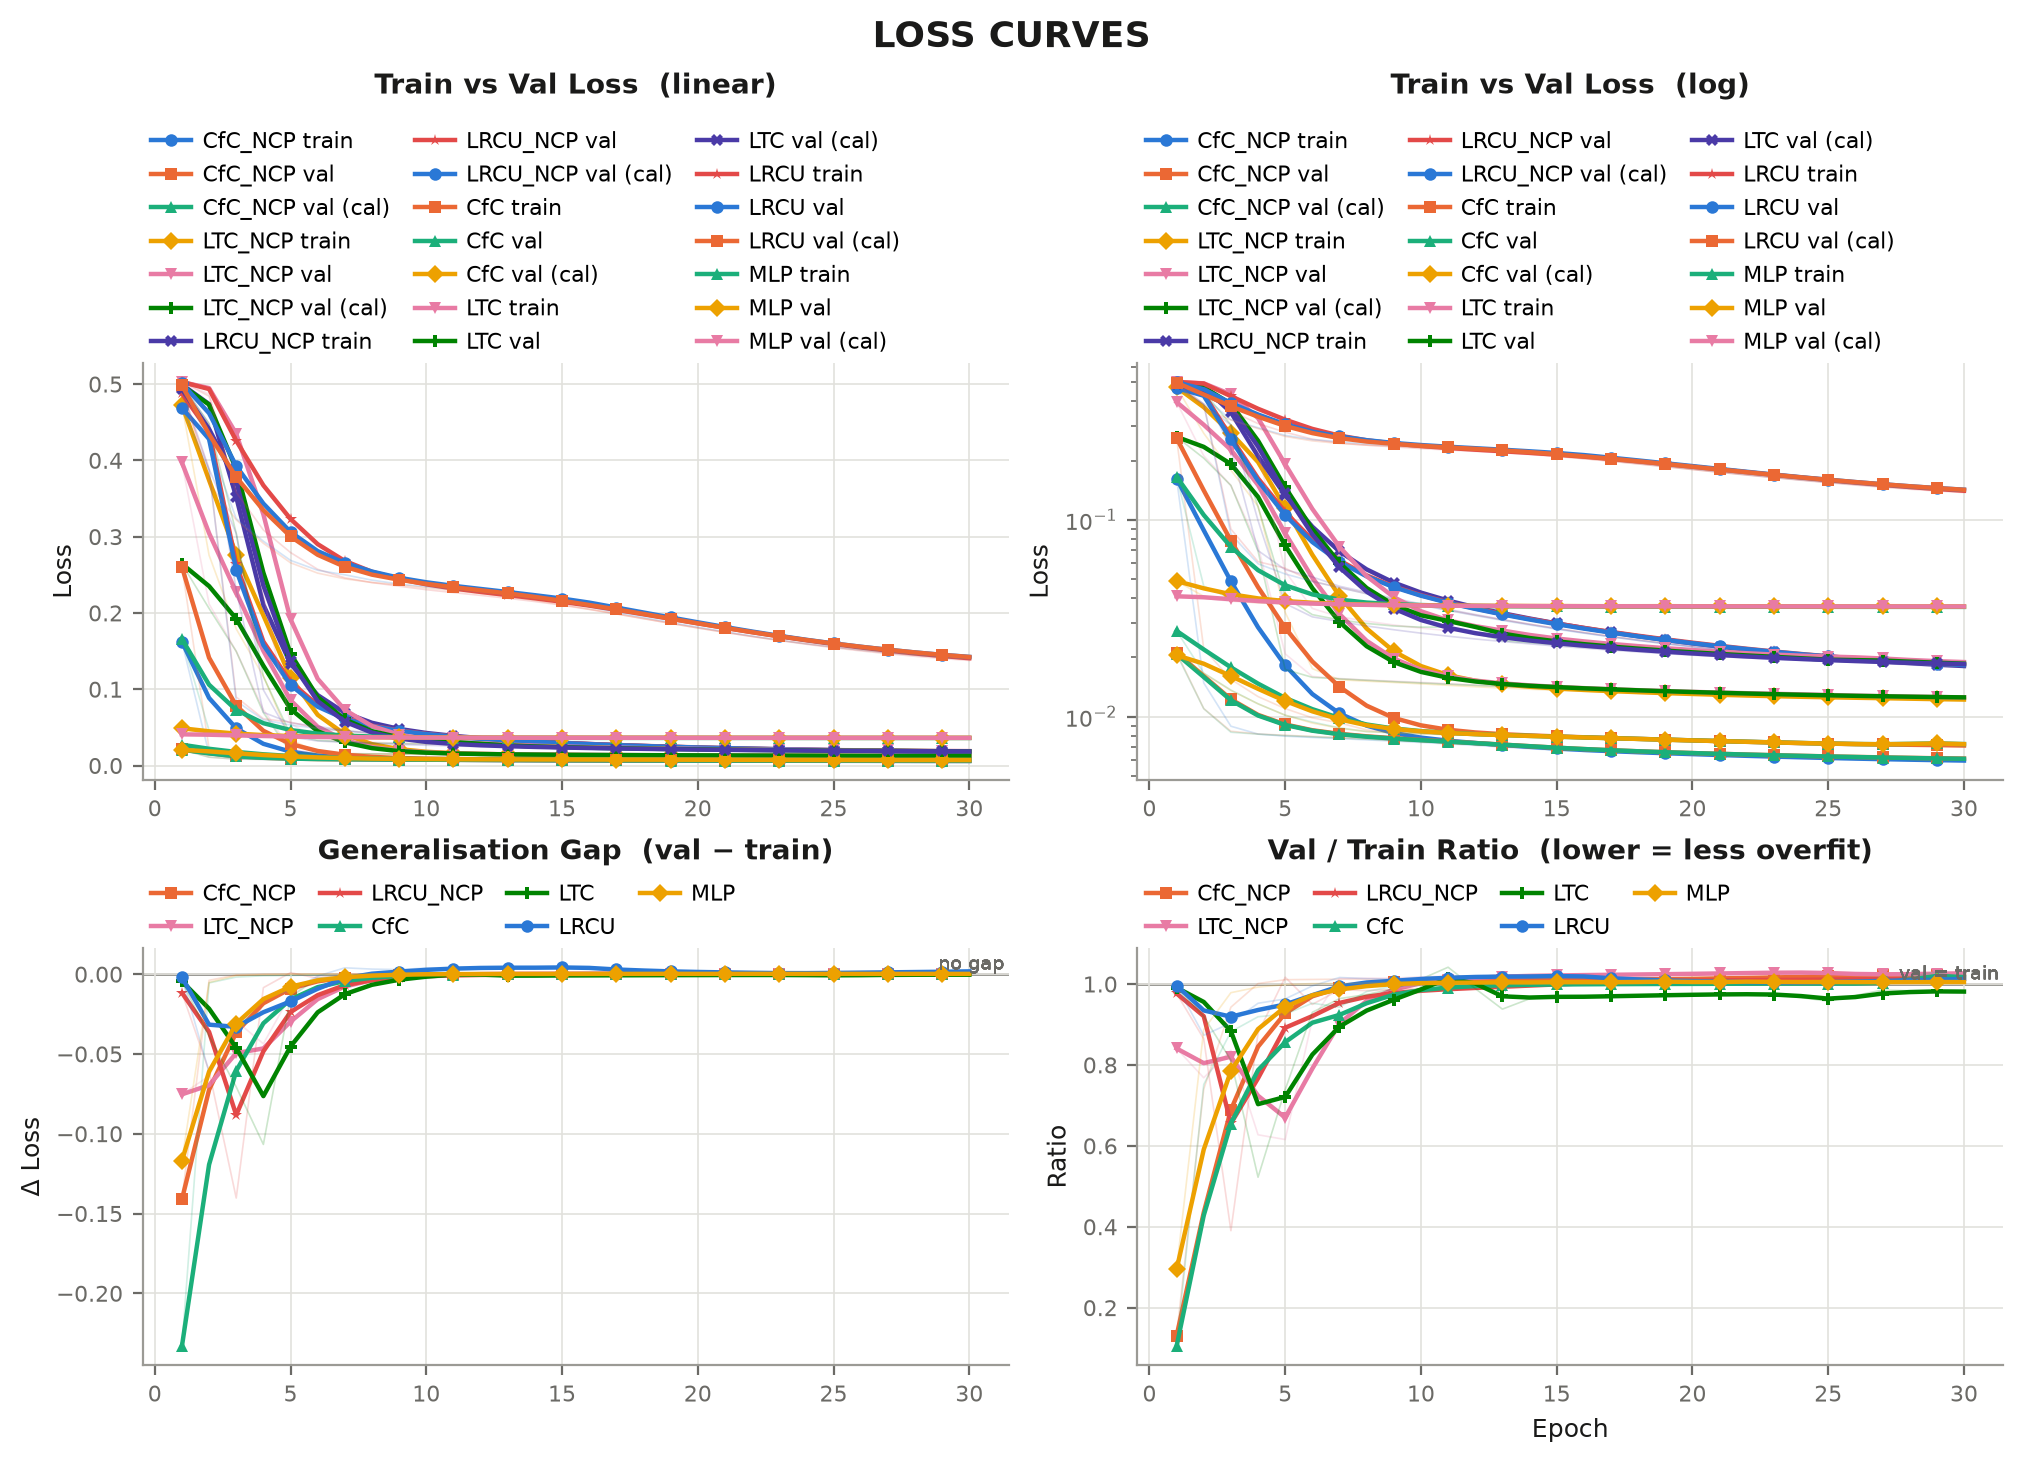
\includegraphics[width=\textwidth]{ch08/sine_losses.png}
  \caption{Synthetic task: training and validation loss on a linear and a
  logarithmic scale (top), and the gap and ratio between validation and
  training (bottom), for the seven vector networks.}
  \label{fig:res-sine-losses}
\end{figure}

\paragraph{What the task does not verify.}
The time step is constant ($\Delta t = 1$), so the task exercises neither the
time argument of the CfC cells nor the interval appended to the observation for
LTC and LRCU (Section~\ref{sec:cell-time}). The task also has a single output
and knows no velocity caps: the cap-scaled loss falls back here to the plain
squared error. What it establishes is that each cell, wired as it will be on the
corpus, learns a known dynamics; everything else is left to the later levels.


\subsection{Training on the Recorded Corpus}
\label{sec:res-sl-corpus}

\paragraph{Setting.}
The seven spatial networks were trained on the recorded corpus with the
run-stratified split of Section~\ref{sec:sl-split}: \num{332} episodes
(\num{77240} frames) for training, \num{74} (\num{16009}) for validation and
\num{70} (\num{17747}) for test, stratified on robot model, world and voxel
size. The corpus contains two robot models --- an unmanned ground vehicle (UGV)
and an unmanned aerial vehicle (UAV) --- and two worlds, and the three
partitions hold them in similar proportions. Every session lasts \num{20}
epochs on windows of \num{16} steps with a stride of \num{4}, batches of
\num{8} sequences, and a learning rate going from $10^{-4}$ to
$1.5\cdot10^{-5}$ with linear decay; an epoch counts \num{1340} measured steps
and lasts between \num{557} and \num{601} seconds, about three and a quarter
hours per session. The remaining settings, read back from the checkpoints'
metadata, are also common to the seven sessions: weights seed and split seed
both $0$, \num{64} archives open at once for the composition of the batch
(Section~\ref{sec:sl-sequences}) with a shuffling reservoir of \num{64}
batches, gradient clipping at a norm of $5$, no position features, and the
auxiliary geometry head enabled with a weight of $0.3$
(Section~\ref{sec:sl-geometry}). Training windows are augmented with the
left--right reflection of Section~\ref{sec:sl-augmentation}.

This subsection describes what the metrics say about the imitation as such,
taking as reference the network that is best in validation,
\met{SparseConv_CfC_NCP}; the comparison between architectures is deferred to
Section~\ref{sec:res-sl-comparison}. All values are read on the epoch selected
as prescribed in Section~\ref{sec:exp-protocol}, that is the one with the
lowest \met{val_loss}. The test partition, read once on the selected
checkpoints, is reported at the end of Section~\ref{sec:res-sl-comparison}.

\paragraph{How the energy of the command is distributed.}
Before reading any error it pays to look at the target. Of the six components
of the command, two --- the roll and pitch rates --- are identically zero across
the whole corpus, and their $R^2$ is undefined. Of the remaining four, the
forward velocity alone carries about 86\% of the energy of the command over the
476 episodes (\num{110996} frames) the sessions were run on, and 84\% and 83\%
in the training and validation partitions respectively (measured as the error
of the zero predictor, the \met{baseline_dim_i} columns); the vertical and yaw
rates share the rest almost equally, about 7\% each, and the lateral velocity
carries less than $0.1\%$. It is this concentration that makes the per-component reading of
Section~\ref{sec:metrics-r2} necessary: a mean loss can be determined almost
entirely by the forward component alone.

The second property of the target that conditions every reading is the share of
frames whose command is identically zero on every component. Over the corpus
it is $12.4\%$, and it is essentially the same for the two platforms
($12.6\%$ for the UGV, $12.2\%$ for the UAV). They are legitimate ``hold still''
targets rather than missing labels, which is why the error on them is reported
separately (Section~\ref{sec:metrics-still}).

\paragraph{The loss against the references.}
The \met{SparseConv_CfC_NCP} reaches its lowest \met{val_loss} at epoch \num{11}
with $4.63\cdot10^{-3}$, that is $3.7\%$ of the zero predictor ($0.126$) and
$35\%$ of the predictor that echoes the observed velocity
($1.31\cdot10^{-2}$). The second comparison is the one that matters: echoing
the velocity is a strong predictor because the command changes slowly, and
beating it by a factor of three says that the network is using the observation
and not merely the velocity the observation already contains.

Read per component, the same network has $R^2 = 0.975$ on the forward velocity,
$0.766$ on the vertical one and $0.982$ on yaw
(Figure~\ref{fig:res-corpus-r2}). The skill against the echo, however, tells a
different story for yaw: it is $0.75$ forward, $0.55$ vertically and
\emph{negative}, $-0.17$, on yaw. The yaw rate in the corpus is so persistent
that echoing it yields a lower error ($3.4\cdot10^{-4}$) than the network's
($4.0\cdot10^{-4}$): the high $R^2$ on that component is to the credit of the
signal's persistence, not of the model. None of the seven networks beats the
echo on yaw (Figure~\ref{fig:res-corpus-skill}).

The lateral component is the opposite case. With less than $0.1\%$ of the
energy, its raw $R^2$ is negative ($-1.6$ for the \met{SparseConv_CfC_NCP},
between $-0.08$ and $-1.6$ for the others): the network produces a lateral
command that is small in absolute terms but large relative to a target that is
almost always zero. The calibration brings the calibrated $R^2$ back to $0.00$
and the amplitude ratio to $0.03$, that is, it effectively switches the axis
off. This is the correct behaviour given the corpus, and it is to be read as an
absence of data on that component, not as learning.

\begin{figure}[htbp]
  \centering
  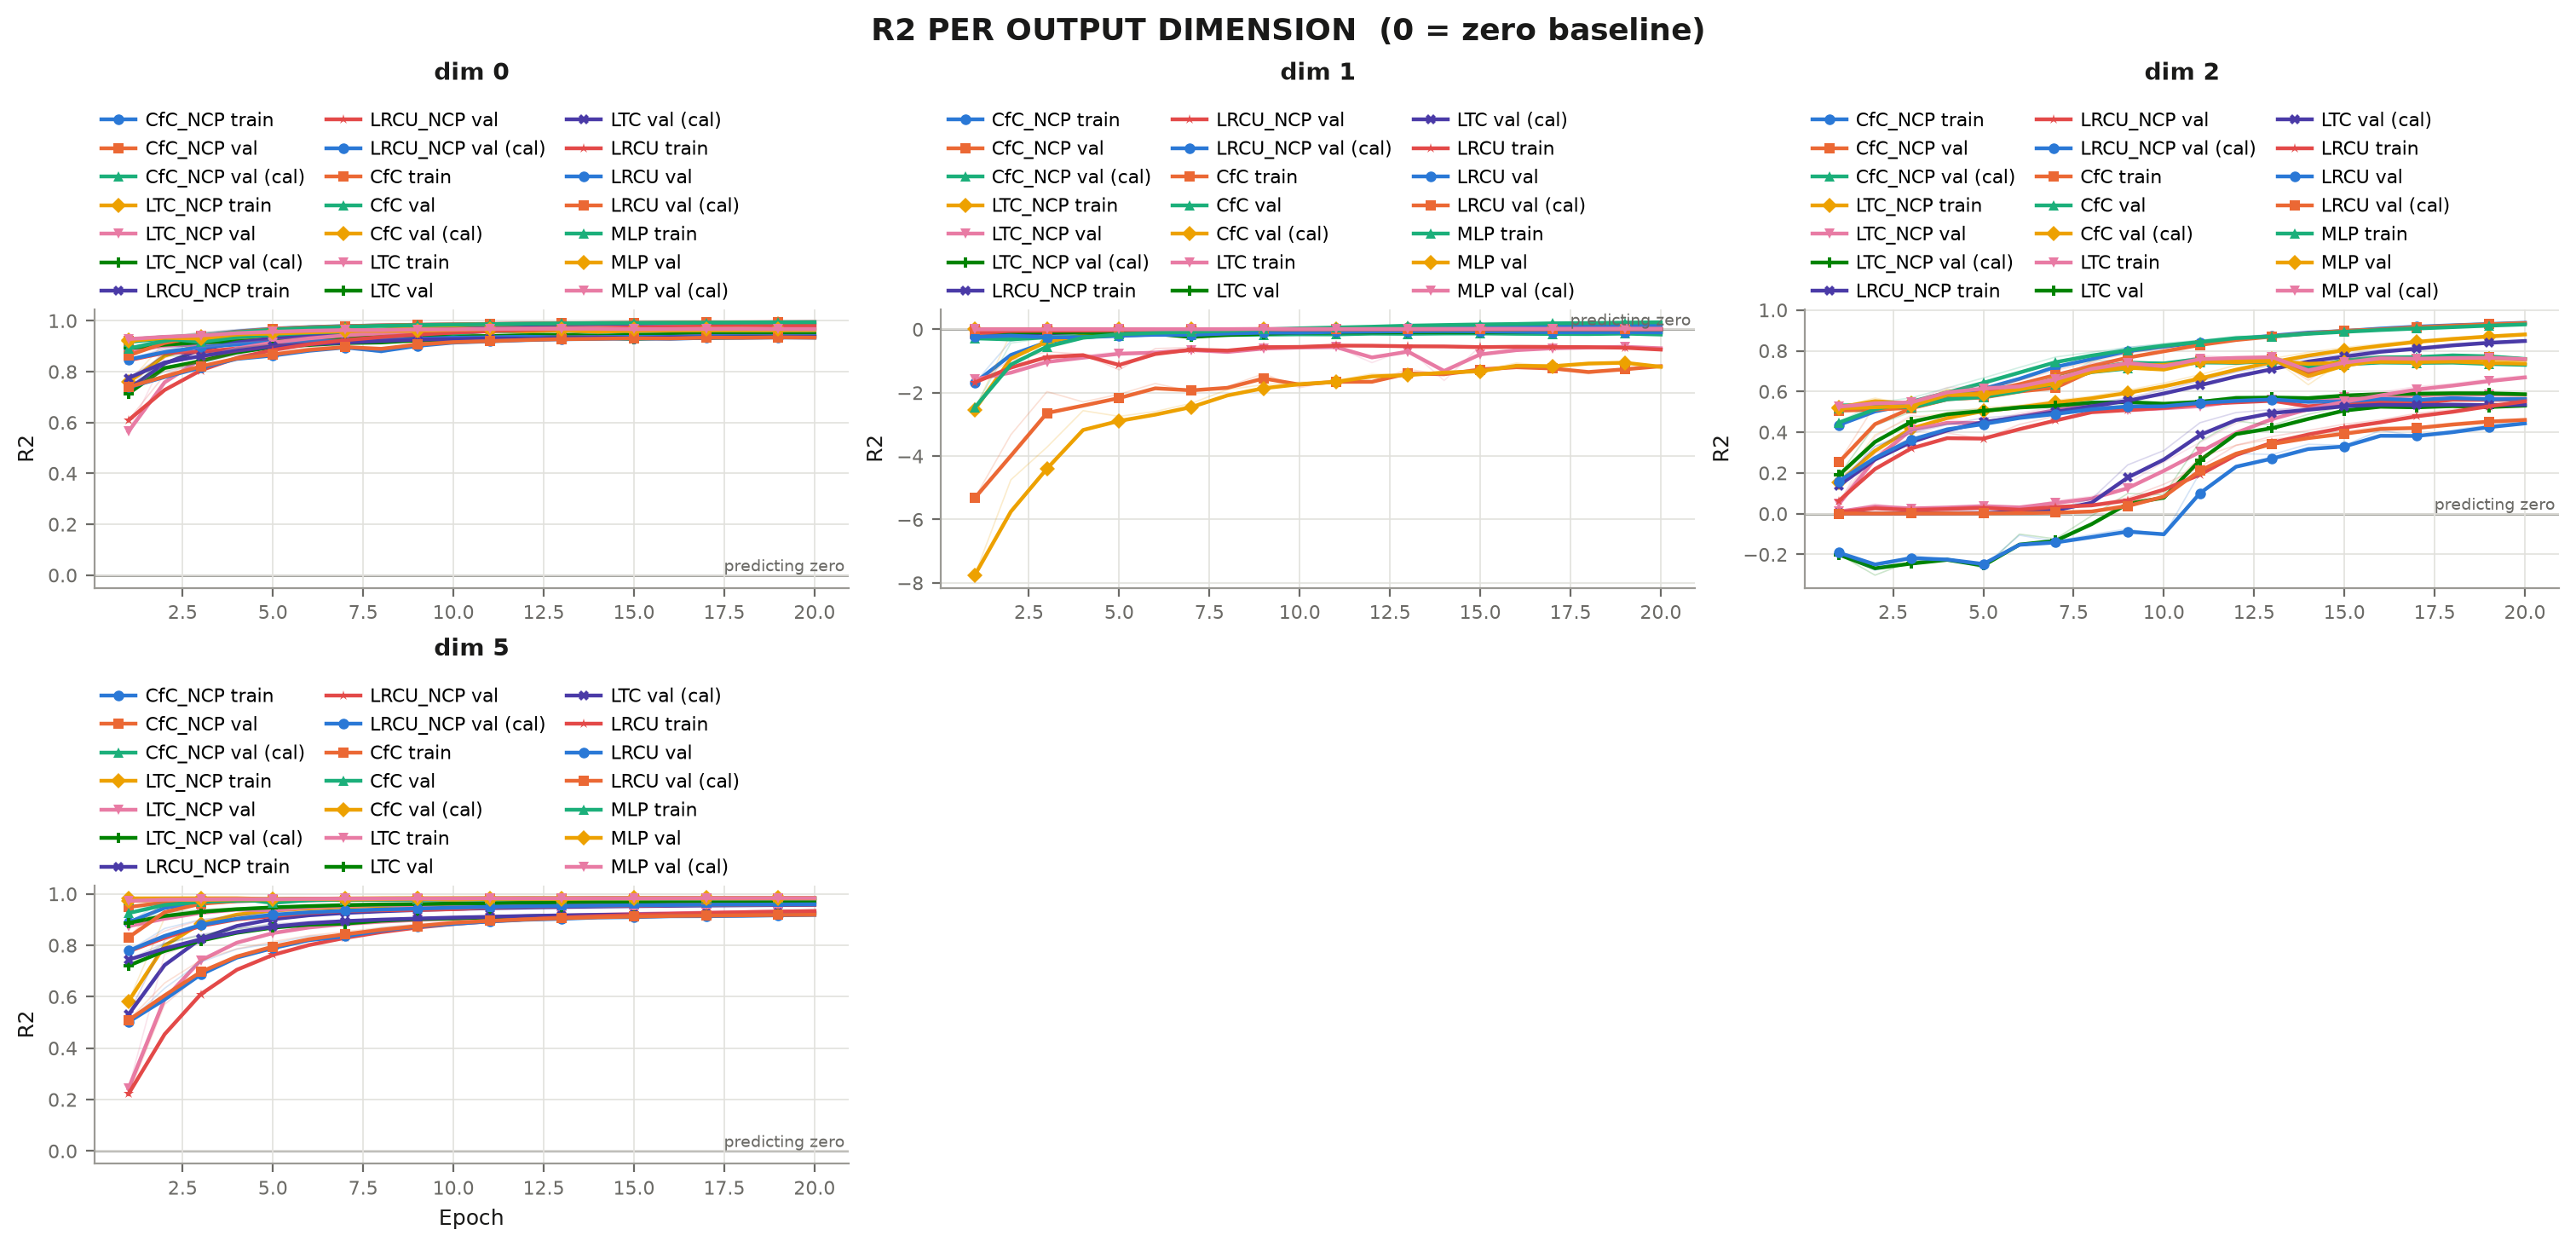
\includegraphics[width=\textwidth]{ch08/corpus_r2_per_dim.png}
  \caption{Corpus: coefficient of determination per component of the command,
  for the seven spatial networks. Components 3 and 4 (roll and pitch rate) are
  zero in the corpus and have no defined $R^2$.}
  \label{fig:res-corpus-r2}
\end{figure}

\begin{figure}[htbp]
  \centering
  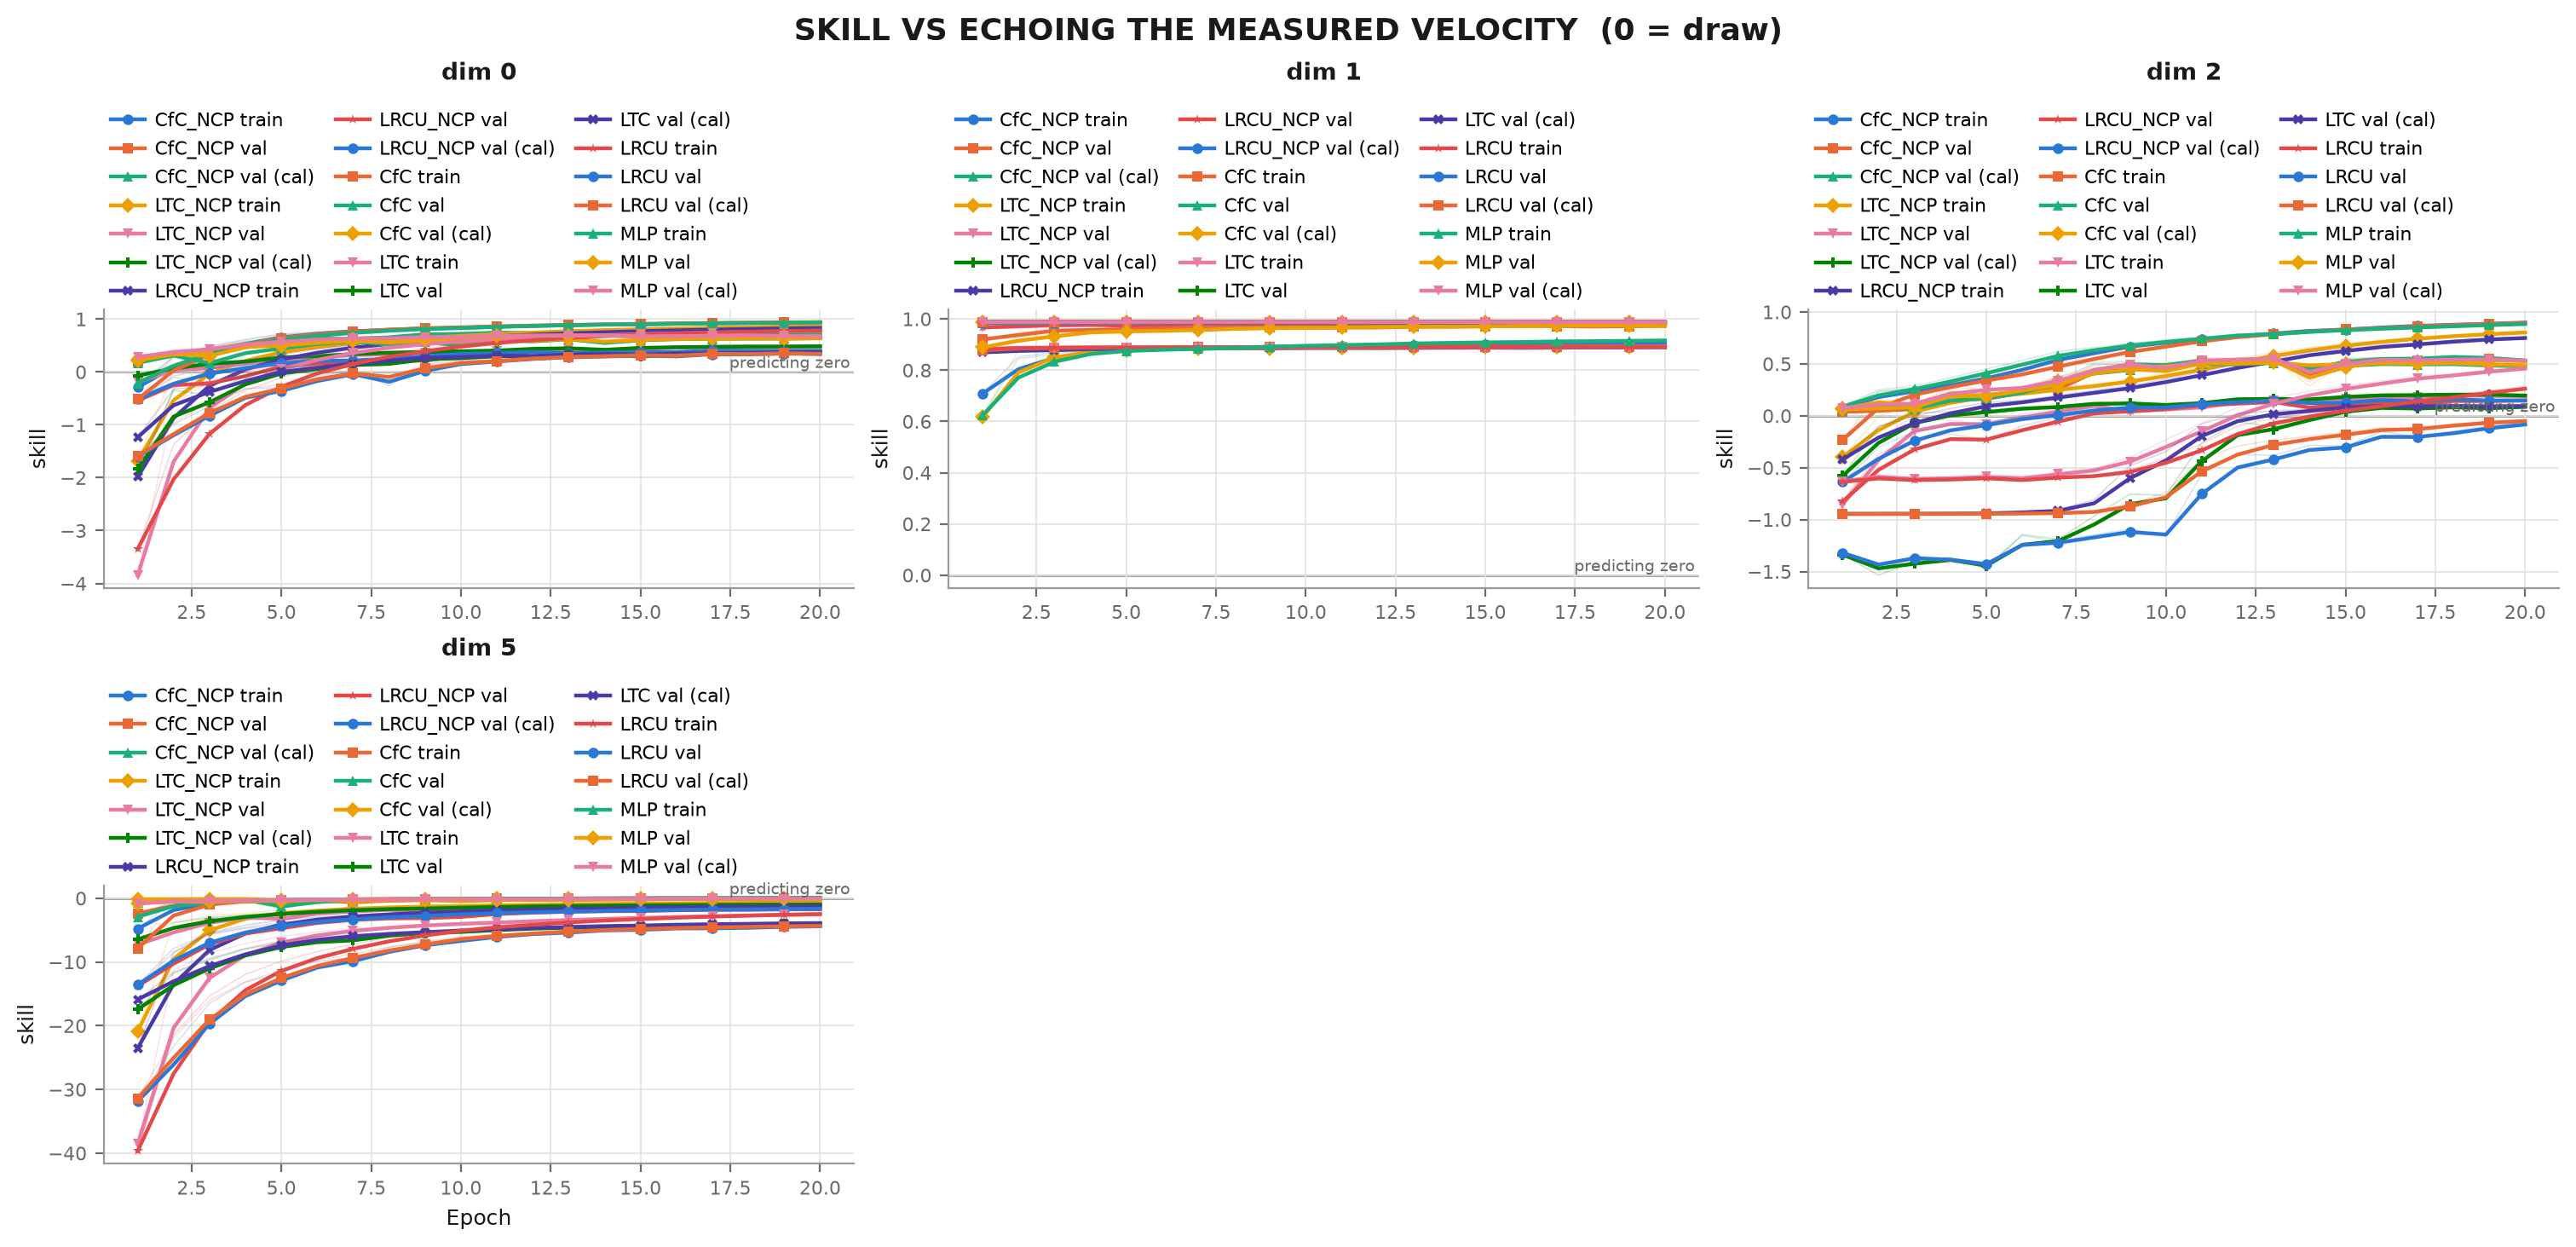
\includegraphics[width=\textwidth]{ch08/corpus_skill_vs_echo.png}
  \caption{Corpus: skill against the predictor that echoes the observed
  velocity, per component. Positive values mean the model beats the echo.}
  \label{fig:res-corpus-skill}
\end{figure}

\paragraph{Amplitude and restart.}
Over all frames the regression towards the mean is limited: the amplitude ratio
of the \met{SparseConv_CfC_NCP} is $0.97$ forward, $0.81$ vertically and $0.97$
on yaw, and the calibration raises the vertical one to $0.88$
(Figure~\ref{fig:res-corpus-amplitude}). The picture changes completely on the
restart frames, where the robot is at rest and the demonstration starts moving.
There the forward restart ratio is $0.02$: the network commands $2\%$ of the
velocity the pilot commanded ($7\cdot10^{-4}$ against
$3.5\cdot10^{-2}$\,\si{\metre\per\second}). Across the seven networks the value
lies between $0.01$ and $0.09$, and the calibration does not move it, because it
corrects the overall spread and not a rare event. On the vertical component the
ratio is higher, between $0.17$ and $0.25$, but it remains far from one.

This is exactly the failure anticipated in
Section~\ref{sec:metrics-amplitude}: at the moment of departure the
demonstration is ambiguous --- the same state of rest sometimes precedes a
departure and sometimes a further wait --- and the least-squares optimum is to
command almost nothing. No architecture solves it by imitation, and it is one of
the reasons why the second training stage exists.

\begin{figure}[htbp]
  \centering
  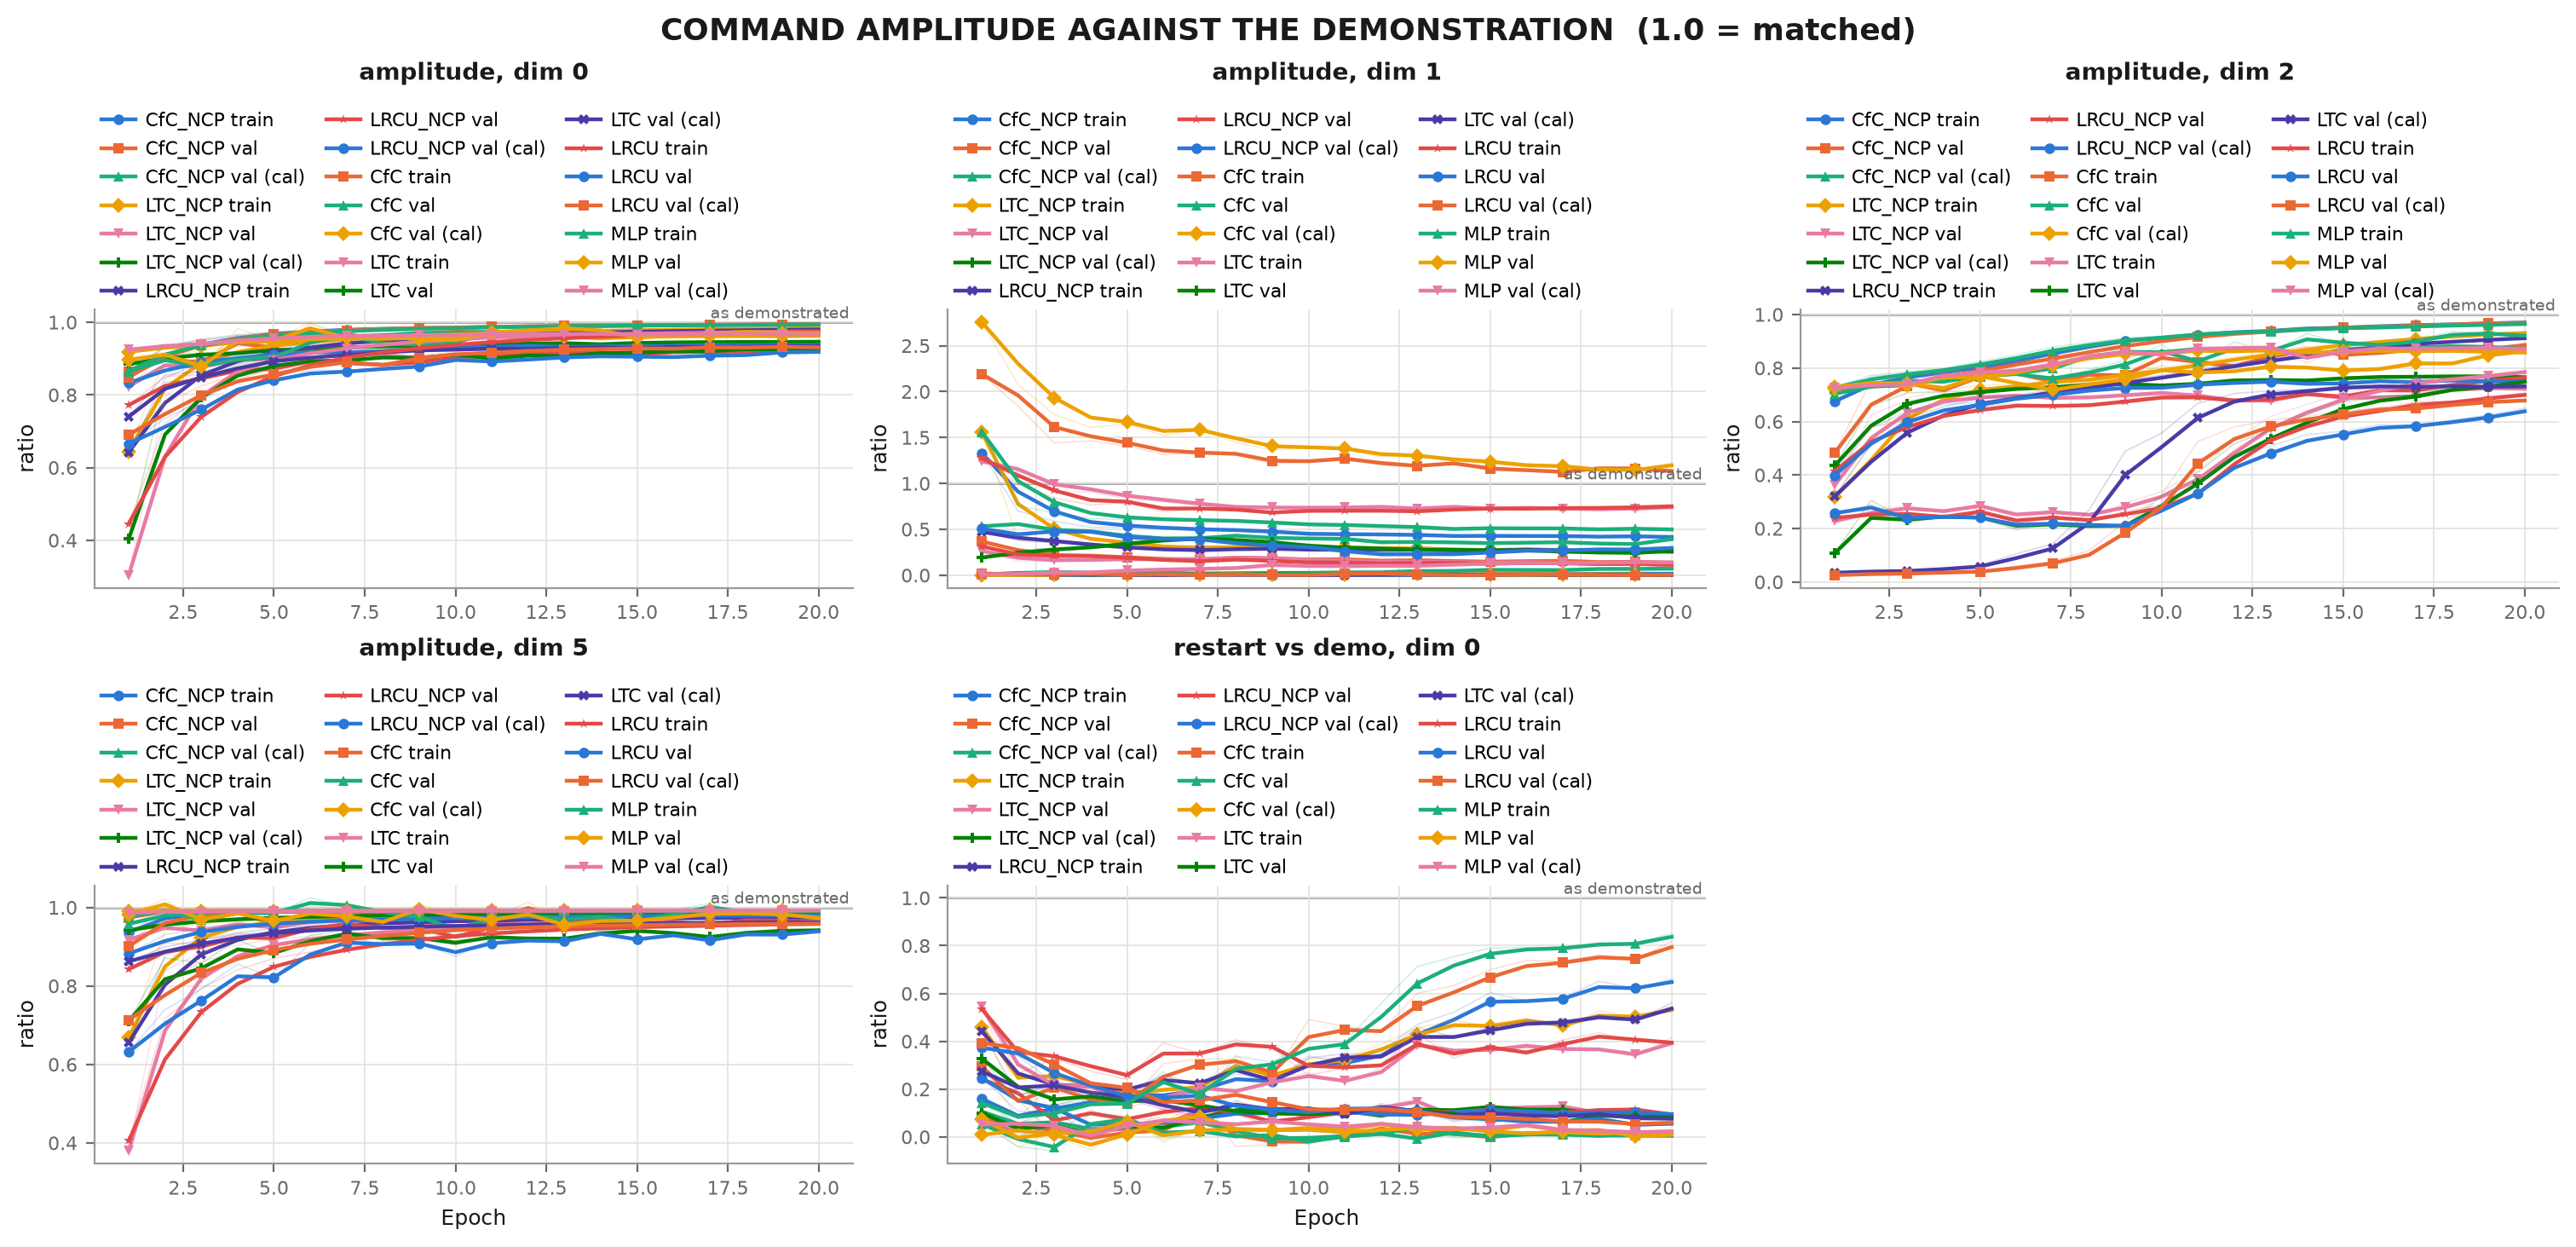
\includegraphics[width=\textwidth]{ch08/corpus_amplitude.png}
  \caption{Corpus: amplitude ratio and restart ratio per component, raw and
  calibrated.}
  \label{fig:res-corpus-amplitude}
\end{figure}

\paragraph{What the selected epoch gives up.}
The protocol of Section~\ref{sec:exp-protocol} selects the epoch of lowest
validation loss, but asks that an epoch improving the loss while degrading the
amplitude or restart metrics be flagged rather than selected in silence. On the
amplitude there is nothing to flag: for every network the selected epoch is
also the one with the largest calibrated amplitude ratio on the forward
component, or within $0.003$ of it. On the restart ratio every network has to
be flagged. The ratio is highest in the first epochs and falls as the loss
falls: from $0.39$ at epoch~1 to $0.06$ at the selected epoch for the
\met{SparseConv_LRCU}, from $0.27$ to $0.07$ for the \met{SparseConv_LTC},
from $0.25$ to $0.09$ for the \met{SparseConv_LRCU_NCP} and from $0.11$ to
$0.01$ for the \met{SparseConv_CfC_NCP} (calibrated values, which are what the
robot executes). Training, in other words, buys part of its loss by commanding
less at departure, which is the behaviour a squared error rewards. The epochs
that command more at a restart have a higher loss --- between $1.4$ and $3.9$
times the selected one --- and choosing them would trade one defect for
another. One exception deserves to be named: for the
\met{SparseConv_LTC_NCP}, epoch~15 has a restart ratio of $0.13$ against
$0.08$ at the selected epoch~20, for a validation loss only 3\% higher. The
selection was nevertheless kept on the loss, as the protocol prescribes; how
much the restart weighs on the fleet is the subject of
Section~\ref{sec:res-cross}.

\paragraph{Still and moving.}
One would expect the frames with a zero command to be the easiest. The opposite
happens: for the \met{SparseConv_CfC_NCP} the per-frame error on still frames
is $5.8\cdot10^{-3}$, against $3.0\cdot10^{-3}$ on moving ones, and for every
network the error on still frames exceeds the error on moving ones, by a factor
between $1.3$ and $2.2$ (Figure~\ref{fig:res-corpus-still}). When the pilot
holds still, the network keeps commanding a small residual velocity. Read
together with the restart ratio, the picture is consistent: around rest the
network errs in both directions, commanding too little when the pilot departs
and a little when the pilot holds still --- it interpolates between the two
cases instead of telling them apart.

\begin{figure}[htbp]
  \centering
  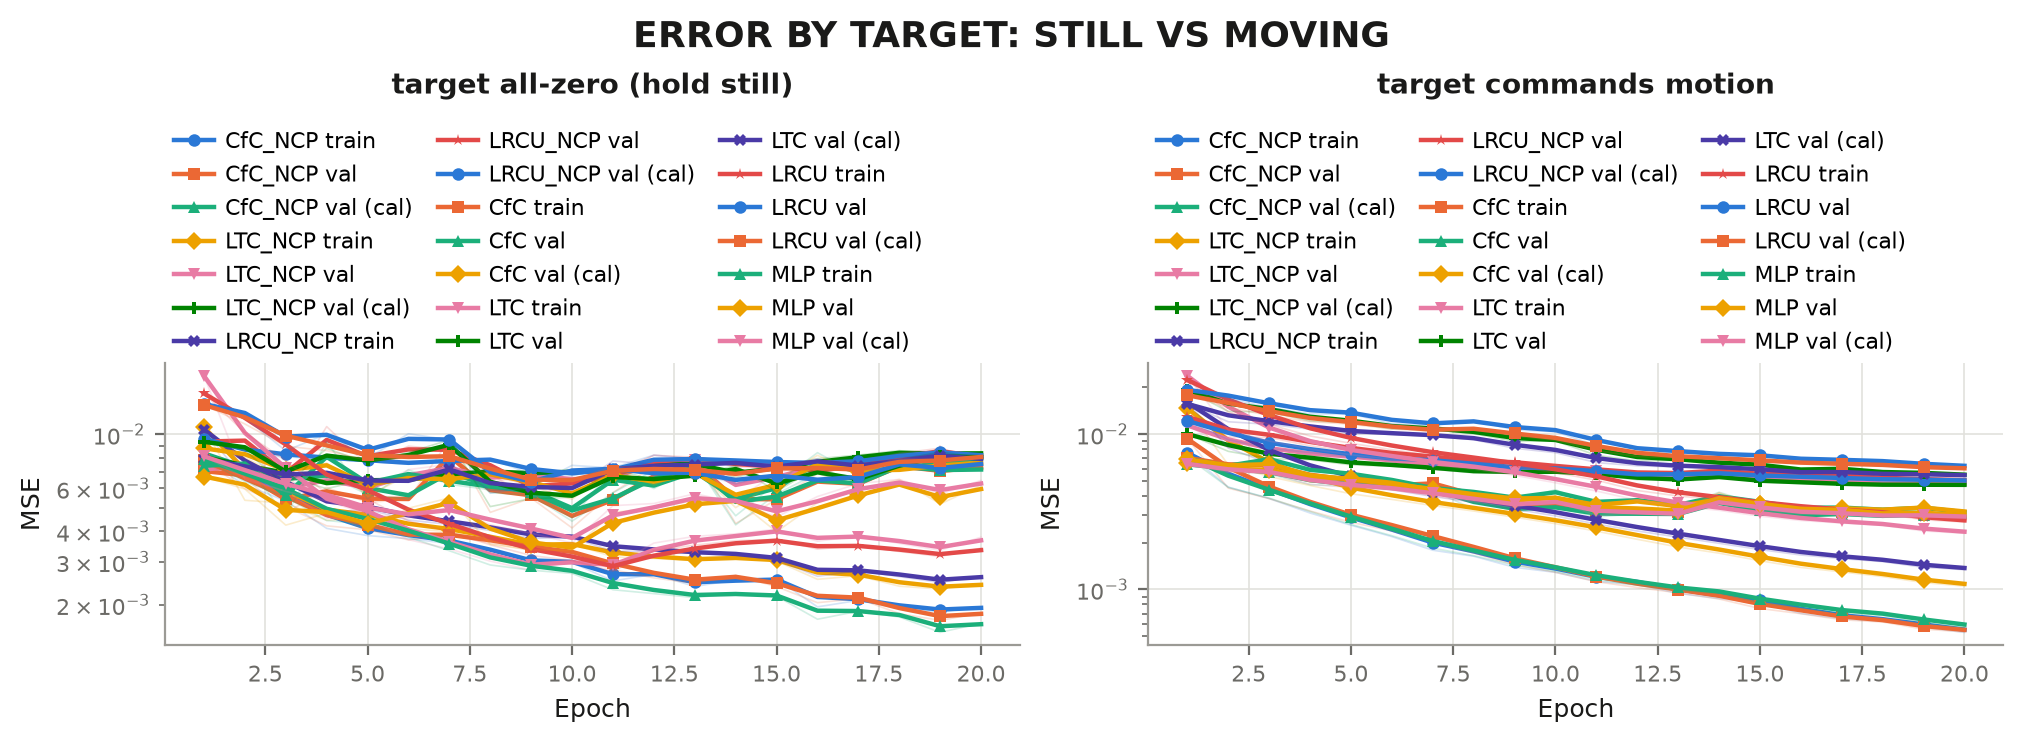
\includegraphics[width=\textwidth]{ch08/corpus_still_vs_moving.png}
  \caption{Corpus: error on frames with a zero command and on frames in
  motion.}
  \label{fig:res-corpus-still}
\end{figure}

\paragraph{Per robot.}
The per-robot breakdown (Section~\ref{sec:metrics-per-robot}) shows neither
platform served worse than the other on the components they share: on the
forward velocity the \met{SparseConv_CfC_NCP} has $R^2 = 0.971$ on the UGV and
$0.978$ on the UAV, on yaw $0.986$ and $0.976$. Only the UAV commands the
vertical component, and the figures on it coincide in practice with the
aggregate ones; the lateral component, which the UGV cannot command, is
practically absent from the UAV's demonstrations as well.

\paragraph{Overfitting.}
On the corpus, unlike on the sine wave, the model memorises. For the
\met{SparseConv_CfC_NCP} the training loss keeps falling until the last epoch,
from $2.9\cdot10^{-3}$ at epoch 11 to $1.6\cdot10^{-3}$ at epoch 20, while the
validation loss stops improving at epoch 11 and then oscillates between $4.8$
and $6.1\cdot10^{-3}$. The ratio between the two rises to about three by the
twentieth epoch (Figure~\ref{fig:res-corpus-losses}). The behaviour is
consistent with a corpus of \num{332} training episodes and with networks sized
for the problem rather than for the corpus
(Section~\ref{sec:networks-implementation}): the excess capacity is spent
memorising the episodes seen. It is also why selecting the checkpoint on the
validation split is not a detail.

\begin{figure}[htbp]
  \centering
  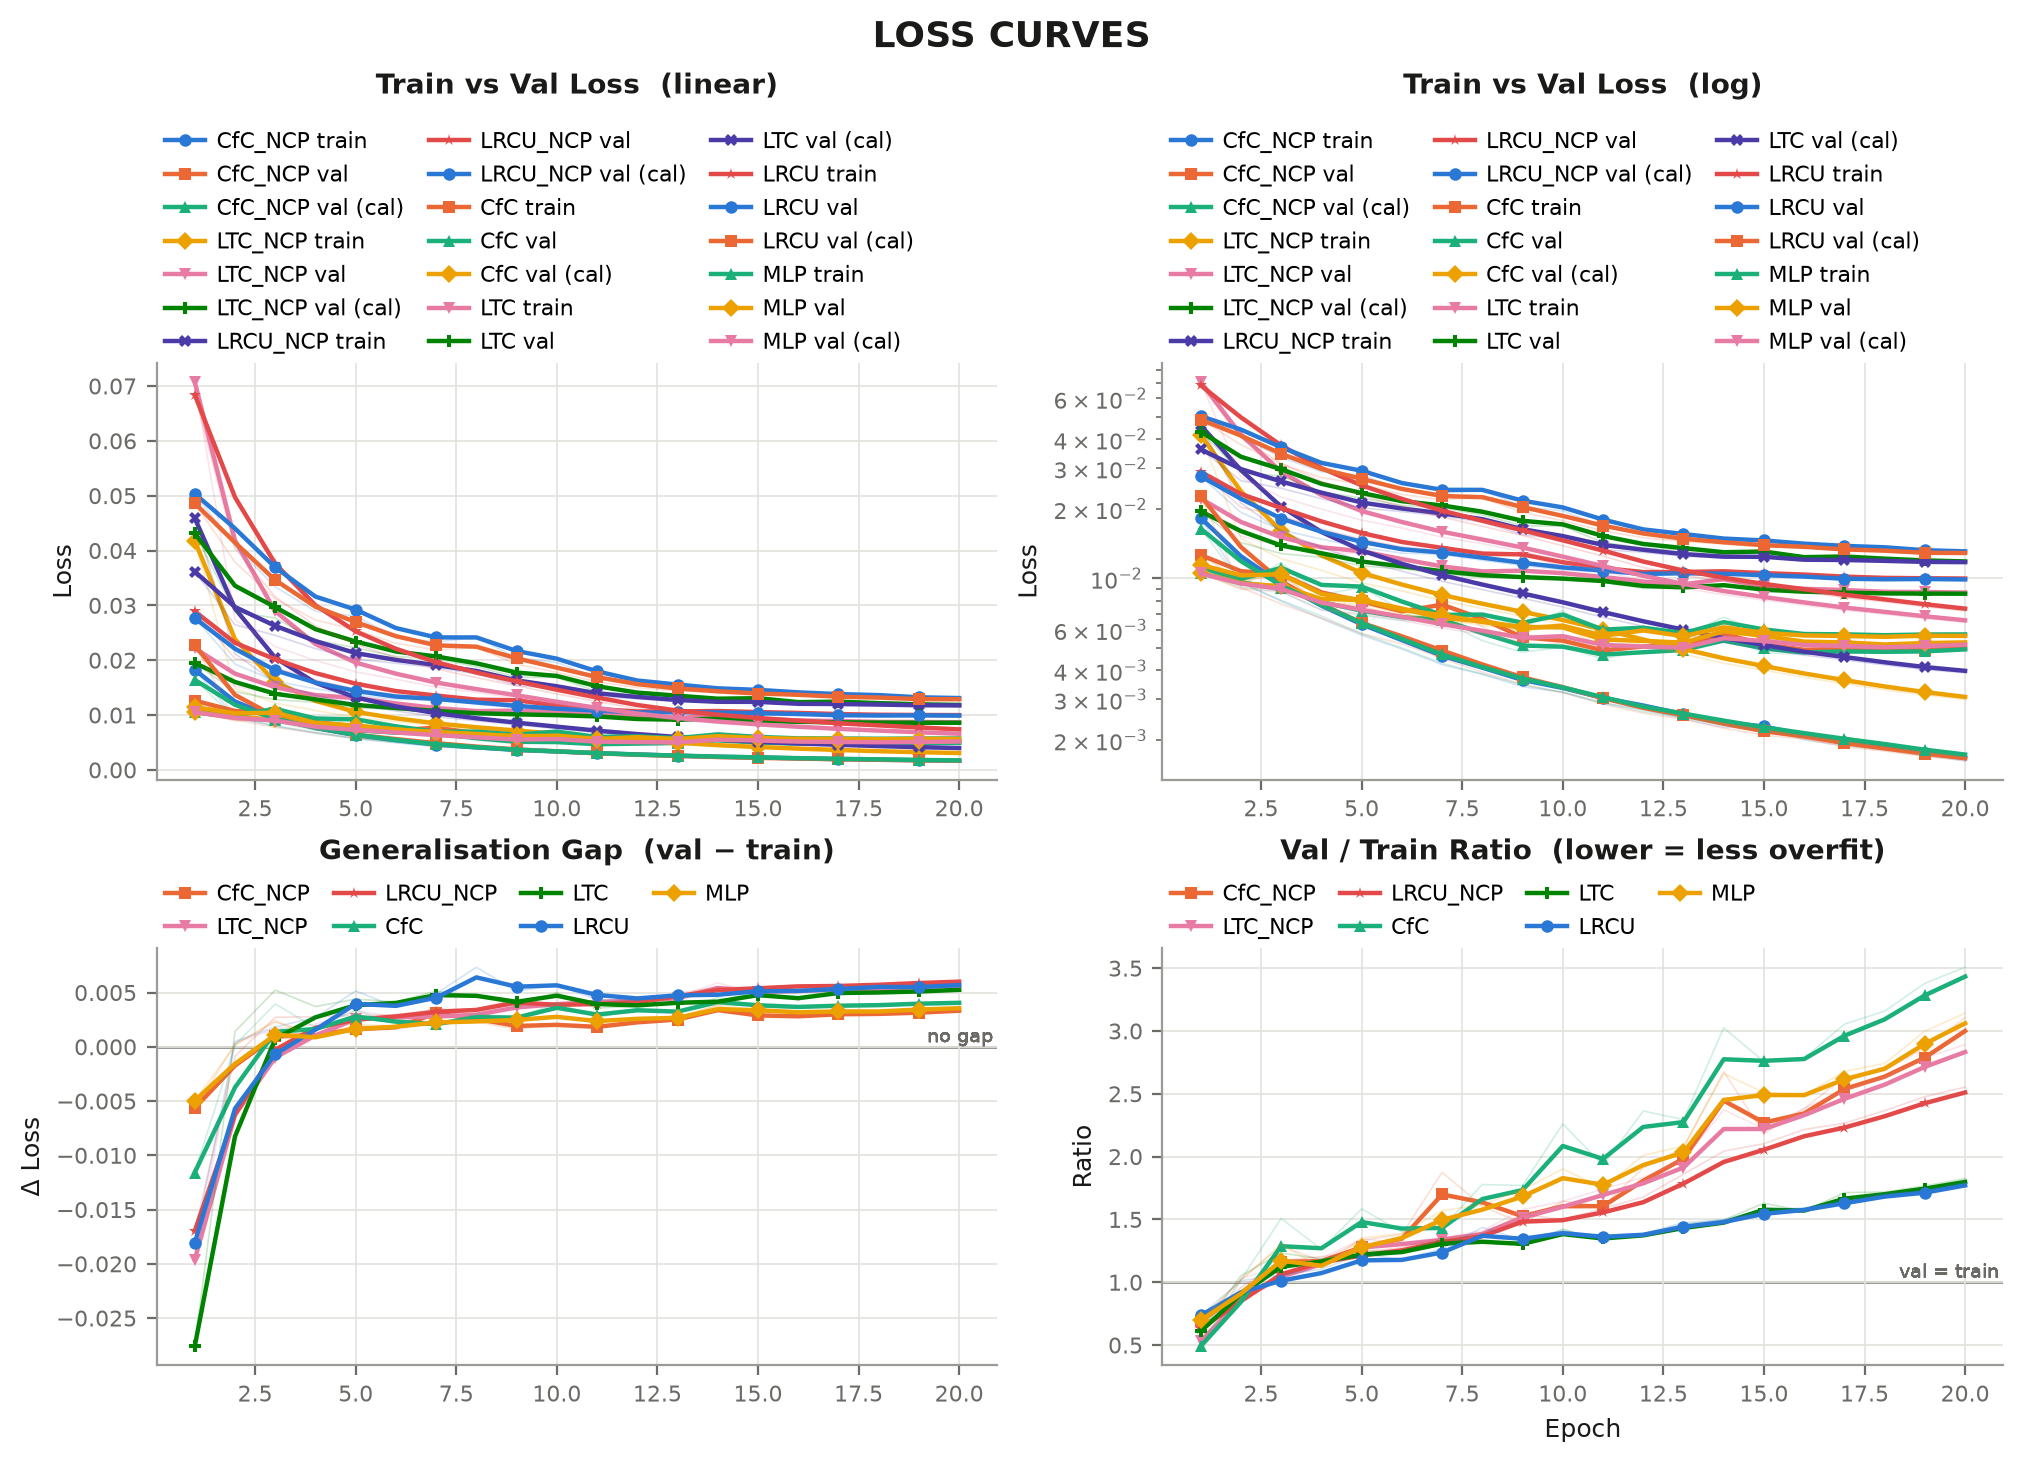
\includegraphics[width=\textwidth]{ch08/corpus_losses.png}
  \caption{Corpus: training and validation loss (top) and their gap and ratio
  (bottom), for the seven spatial networks.}
  \label{fig:res-corpus-losses}
\end{figure}


\subsection{Architecture Comparison}
\label{sec:res-sl-comparison}

Table~\ref{tab:res-corpus} compares the seven networks at the epoch of lowest
\met{val_loss}, under the conditions of Section~\ref{sec:exp-protocol}: same
corpus, same split, same seed, same schedule, same state widths.

\begin{table}[htbp]
  \centering
  \small
  \caption{Corpus: comparison of the architectures at the epoch of lowest
  validation loss. Losses in units of $10^{-3}$; $R^2$, skill and restart
  ratio on the forward component ($v_x$) unless stated otherwise, on raw
  values. Zero predictor $126.4$, velocity echo $13.1$.}
  \label{tab:res-corpus}
  \setlength{\tabcolsep}{4pt}
  \begin{tabular}{@{}lrrrrrrrr@{}}
    \toprule
    \textbf{Network} & \textbf{Ep.} & \met{val_loss} & \textbf{cal.} & $R^2_{v_x}$ & $R^2_{v_z}$ & $R^2_{\omega_z}$ & \textbf{Skill} & \textbf{Restart} \\
    \midrule
    \met{CfC_NCP}  & 11 &  4.63 &  4.49 & 0.975 & 0.766 & 0.982 & 0.75 & 0.02 \\
    \met{MLP} (ctrl.) & 11 &  5.09 &  4.92 & 0.969 & 0.766 & 0.982 & 0.69 & 0.03 \\
    \met{CfC}      & 11 &  5.52 &  5.35 & 0.965 & 0.752 & 0.981 & 0.65 & 0.01 \\
    \met{LTC_NCP}  & 20 &  8.67 &  8.58 & 0.948 & 0.582 & 0.969 & 0.49 & 0.09 \\
    \met{LRCU_NCP} & 20 &  9.98 &  9.88 & 0.939 & 0.562 & 0.959 & 0.40 & 0.08 \\
    \met{LTC}      & 20 & 11.78 & 11.74 & 0.936 & 0.534 & 0.926 & 0.37 & 0.08 \\
    \met{LRCU}     & 20 & 13.03 & 12.87 & 0.933 & 0.453 & 0.919 & 0.33 & 0.06 \\
    \bottomrule
  \end{tabular}
\end{table}

\paragraph{Two groups.}
The networks split sharply into two groups. The two CfC networks and the control
reach their minimum at epoch 11 with losses between $4.6$ and
$5.5\cdot10^{-3}$, and then overfit. The four LTC and LRCU networks are instead
still descending at the last epoch, with losses $1.9$ to $2.8$ times higher,
and the \met{SparseConv_LRCU} barely matches the velocity echo ($13.0$ against
$13.1\cdot10^{-3}$). The split is the same observed on the sine wave --- CfC
converges within one or two epochs, LTC and LRCU start slowly --- and it is to
be read with the same caution: after twenty epochs the second group has not yet
reached its own minimum, and a comparison at a fixed budget measures in part the
speed of convergence rather than the capacity. Separating the two would require
continuing the LTC and LRCU sessions until their validation loss turns, which
was not done. The skill on yaw follows the two groups too: between $-0.17$ and
$-0.24$ for the first, between $-1.0$ and $-4.4$ for the second.

\paragraph{The stateless control.}
The most relevant result of the comparison is where the control stands. The
\met{SparseConv_MLP}, identical to the others but with two linear layers in
place of the cells and therefore without memory from one step to the next, comes
second: its validation loss is $10\%$ higher than that of the
\met{SparseConv_CfC_NCP} and lower than that of the \met{SparseConv_CfC}, and
its per-component figures are in practice indistinguishable from those of the
two CfC networks. The difference between the best recurrent network and the
control, $0.46\cdot10^{-3}$, is smaller than the oscillation of the
\met{SparseConv_CfC_NCP} itself from one epoch to the next after its minimum
(between $4.8$ and $6.1\cdot10^{-3}$), and each configuration was run with a
single seed. Under the rule of Section~\ref{sec:exp-protocol}, then, the
advantage of the \met{SparseConv_CfC_NCP} over the control is indicative, not
established; what this means for the comparison as a whole is discussed in
Section~\ref{sec:res-discussion}.

\paragraph{Wiring.}
For the same cell, the NCP variant is better in all three cases: $4.63$ against
$5.52$ for CfC, $8.67$ against $11.78$ for LTC, $9.98$ against $13.03$ for LRCU.
For LTC and LRCU the difference, about a quarter of the loss, exceeds the
epoch-to-epoch oscillation; for CfC it is of the same order. The NCP wiring also
brings the two skip connections from the input to the second cell and from the
first cell to the output (Section~\ref{sec:lnn-wiring}), which shorten the
gradient path: with the data available the gain cannot be attributed to the
sparsity of the wiring rather than to the skips.

\paragraph{Cost.}
The cost per epoch varies little, between \num{557} seconds for the control and
\num{601} for the \met{SparseConv_LRCU_NCP}: on the corpus the time is dominated
by the encoder and by data loading, not by the cells. Nor does the parameter
count (Table~\ref{tab:architectures}) explain the ranking: the
\met{SparseConv_LRCU_NCP} is the largest network and comes fifth, the control is
the smallest and comes second.

\paragraph{The held-out test.}
The validation partition was used twice to decide --- to select the epoch and
to fit the calibration --- so its figures are not an unbiased estimate
(Section~\ref{sec:exp-protocol}). The test partition, which took part in
neither decision, was read once, on the seven selected checkpoints and after
the comparison above had been written: raw, with the calibration at the
identity, and calibrated, through the coefficients each checkpoint had fitted
on validation, which is the output the robot would receive.
Table~\ref{tab:res-test} reports it.

\begin{table}[htbp]
  \centering
  \small
  \caption{Corpus: the selected checkpoints on the held-out test partition
  (70 episodes, \num{17747} frames), read once. Losses in units of $10^{-3}$;
  the validation loss is repeated for reference. $R^2$ and skill on the raw
  output; skill on the forward component and on yaw. Zero predictor $127.7$,
  velocity echo $13.9$.}
  \label{tab:res-test}
  \setlength{\tabcolsep}{4pt}
  \begin{tabular}{@{}lrrrrrrrr@{}}
    \toprule
    \textbf{Network} & \textbf{val} & \textbf{test} & \textbf{cal.} & $R^2_{v_x}$ & $R^2_{v_z}$ & $R^2_{\omega_z}$ & \textbf{Skill} $v_x$ & \textbf{Skill} $\omega_z$ \\
    \midrule
    \met{CfC_NCP}     &  4.63 &  4.66 &  4.55 & 0.973 & 0.805 & 0.978 & 0.72 & $-0.16$ \\
    \met{MLP} (ctrl.) &  5.09 &  4.99 &  4.83 & 0.971 & 0.783 & 0.978 & 0.70 & $-0.17$ \\
    \met{CfC}         &  5.52 &  5.17 &  4.94 & 0.969 & 0.781 & 0.977 & 0.68 & $-0.20$ \\
    \met{LTC_NCP}     &  8.67 &  7.98 &  7.91 & 0.955 & 0.619 & 0.965 & 0.54 & $-0.84$ \\
    \met{LRCU_NCP}    &  9.98 &  9.39 &  9.34 & 0.948 & 0.575 & 0.952 & 0.47 & $-1.51$ \\
    \met{LTC}         & 11.78 & 12.08 & 12.06 & 0.939 & 0.513 & 0.912 & 0.37 & $-3.61$ \\
    \met{LRCU}        & 13.03 & 12.55 & 12.45 & 0.942 & 0.443 & 0.908 & 0.40 & $-3.83$ \\
    \bottomrule
  \end{tabular}
\end{table}

Three things follow from it. The first is that the validation figures were not
flattered by being used to decide: for every network the test loss lies within
8\% of the validation loss, in both directions, and the ranking of the seven is
the same on the two partitions. The second is that the calibration fitted on
validation carries over to data it has never seen: the calibrated test loss is
lower than the raw one for all seven networks, by up to 4\% for the
\met{SparseConv_CfC}, and on the lateral component it again brings a negative
raw $R^2$ back to zero. The third is that none of the readings of this section
is an artefact of the validation partition. The best recurrent network and the
control remain separated by less than the epoch-to-epoch fluctuation ($4.66$
against $4.99$); no network beats the echo on yaw; the restart ratio is, if
anything, lower still, at most $0.07$ and slightly negative for the control; the
error on still frames exceeds the error on moving ones by a factor between
$1.6$ and $3.0$; and the forward $R^2$ stays between $0.93$ and $0.98$ on both
platforms.


\subsection{What the Encoder Learns}
\label{sec:res-sl-encoder}

The sections above read the command; this one reads the encoder that feeds it,
on the validation partition and for all seven networks. Three measurements are
available, and they answer questions of increasing strictness. The first is the
auxiliary head itself (Section~\ref{sec:geometry-head}): at the selected epoch
it explains about $47$--$50\%$ of the variance of the per-sector clearances and
$69$--$81\%$ of that of the height. That figure is an upper reading of what the
encoder represents, because the head is non-linear and trained together with
the encoder. The two tools of Section~\ref{sec:exp-tooling} ask the stricter
questions: whether the command actually \emph{uses} what the encoder computes ---
the ablation --- and whether a \emph{linear} read-out of the frozen descriptor,
fitted on some episodes and scored on others, recovers the geometry --- the
probe. The probe's figures are therefore lower than the head's, and they are the
ones to read.

\paragraph{Does the command use the map?}
The ablation replaces, with the same weights, the encoder's per-sample output
by its batch mean --- the information is gone, the fusion stays in the range it
was trained on --- and measures the calibrated validation loss again
(Table~\ref{tab:res-encoder}). The loss rises for all seven networks, from
$+8\%$ for the \met{SparseConv_LRCU} to $+22\%$ for the two CfC networks, and
it rises further, by $14$--$48\%$, when every observation is given another
sample's cloud instead. The command therefore depends on the content of the
cloud and not merely on its presence as a constant, and the better a network
imitates, the more it relies on it. The dependence is at least as strong on the
$143^3$ grid, the one the fleet flies ($+7$ to $+25\%$). Per component, what the
map carries is mostly the vertical command: for the \met{SparseConv_CfC_NCP}
its $R^2$ falls from $0.77$ to $0.72$ without the encoder, the forward one from
$0.975$ to $0.968$, and the yaw one does not move. The finest grid, $363^3$,
holds only UGV frames with a residual loss four times smaller than the others,
and there the percentages scatter between $-35\%$ and $+146\%$; it is not read.

\paragraph{Does the encoder represent the scene?}
The probe answers the second question independently of the command: a ridge
regression from the frozen descriptor to the geometry each frame's own cloud
shows --- the clearance per azimuth sector and the height above the ground ---
fitted on half of the validation episodes and scored on the other half, so that
a descriptor identifying the episode rather than describing the scene gains
nothing. The same architecture at its initialisation gives the floor a trained
read-out must clear (Table~\ref{tab:res-encoder}). Untrained, the descriptor
already explains $24\%$ of the variance of the sector clearances and $43\%$ of
that of the height, which is what a random sparse convolution preserves of a
point cloud. Trained, the seven encoders reach $37$--$44\%$ on the sectors and
$68$--$75\%$ on the height, with differences between architectures that are
small and do not follow their ranking in the loss: the encoder is the same for
all of them, and what the cells do downstream does not change what it learns.
The height is the less telling of the two figures, since it separates the two
platforms before anything else --- the UGV sits at a fixed height, the UAV
cruises --- and a descriptor that recognises the robot explains most of it.

The sector clearances are the figure that matters for the fleet, and on the
$143^3$ grid the fleet flies they are the weakest: between $0.15$ and $0.29$
against an untrained floor of $0.15$, so that for some networks the directional
distance to the obstacles is barely more readable after training than before.
Training does make the descriptor more informative in the other two respects the
probe measures: its spread across samples grows from $0.07$ to $0.16$--$0.22$ on
that grid, and its displacement under a shift of three voxels falls from $0.80$
to $0.44$--$0.58$ of the distance between two different clouds. Taken together
with the ablation, the picture is consistent: the imitation uses the map, it
uses it mostly for the vertical command, and it teaches the encoder where the
obstacles are only in part --- the part the reinforcement stage has to build on.

\begin{table}[htbp]
  \centering
  \small
  \caption{Corpus: what the command takes from the encoder and what the
  encoder represents, on the validation partition. \emph{Ablation}: increase of
  the calibrated loss when the encoder's output is replaced by its batch mean,
  overall and on the $143^3$ grid the fleet flies, and when the clouds are
  shuffled across the batch. \emph{Probe}: fraction of the variance of the
  sector clearances and of the height explained by a linear read-out of the
  frozen descriptor, on held-out episodes; the last row is the same
  architecture at its initialisation.}
  \label{tab:res-encoder}
  \setlength{\tabcolsep}{4pt}
  \begin{tabular}{@{}lrrrrrr@{}}
    \toprule
    & \multicolumn{3}{c}{\textbf{Ablation}} & \multicolumn{3}{c}{\textbf{Probe}} \\
    \cmidrule(lr){2-4}\cmidrule(l){5-7}
    \textbf{Network} & \textbf{Mean} & \textbf{Mean, $143^3$} & \textbf{Shuffled} & \textbf{Sectors} & \textbf{Sectors, $143^3$} & \textbf{Height} \\
    \midrule
    \met{CfC_NCP}     & $+21.9\%$ & $+24.9\%$ & $+40.5\%$ & 0.40 & 0.18 & 0.70 \\
    \met{MLP} (ctrl.) & $+18.8\%$ & $+20.4\%$ & $+47.9\%$ & 0.40 & 0.19 & 0.73 \\
    \met{CfC}         & $+22.4\%$ & $+22.5\%$ & $+39.0\%$ & 0.42 & 0.29 & 0.71 \\
    \met{LTC_NCP}     & $+15.3\%$ & $+19.6\%$ & $+32.1\%$ & 0.44 & 0.15 & 0.73 \\
    \met{LRCU_NCP}    & $+13.7\%$ & $+21.1\%$ & $+24.3\%$ & 0.37 & 0.21 & 0.75 \\
    \met{LTC}         & $+11.2\%$ & $+13.7\%$ & $+17.6\%$ & 0.44 & 0.20 & 0.72 \\
    \met{LRCU}        &  $+8.2\%$ &  $+7.3\%$ & $+14.3\%$ & 0.43 & 0.22 & 0.68 \\
    \midrule
    untrained         & -- & -- & -- & 0.24 & 0.15 & 0.43 \\
    \bottomrule
  \end{tabular}
\end{table}


\section{Reinforcement Learning}
\label{sec:res-rl}

\subsection{Validation on LunarLander}
\label{sec:res-rl-lunar}

\paragraph{Setting.}
The recurrent agent was verified on the LunarLander environment of
\texttt{gymnasium} (version~3), with a dense eight-component observation and
four discrete actions, without the fleet. The seven vector networks are trained
from scratch on \num{16} parallel environments, with rollouts of \num{512} steps
per environment, that is \num{8192} transitions per iteration, for \num{733}
iterations and about \num{6.0} million steps. The six recurrent networks share
a single configuration (Section~\ref{sec:rl-presets}): windows of \num{32}
steps, six epochs per update, a target KL of $0.02$, a clipping $\epsilon$
annealed from $0.2$ to $0.08$ and a learning rate going from $2\cdot10^{-4}$ to
$6\cdot10^{-5}$. The control has its own configuration but the same step
budget, so that the curves are comparable along the horizontal axis. Each
network was run once. The external reference is the conventional threshold of
$200$ mean return, above which LunarLander is considered solved; times to
threshold are read on a moving average over twenty iterations.

\begin{table}[htbp]
  \centering
  \small
  \caption{LunarLander: steps to threshold (millions, moving average over 20
  iterations), mean return, episode length and worst episodic return over the
  last 50 iterations, wall-clock duration of the session, and largest recorded
  norm of the recurrent state.}
  \label{tab:res-lunar}
  \setlength{\tabcolsep}{4pt}
  \begin{tabular}{@{}lrrrrrrr@{}}
    \toprule
    \textbf{Network} & $\geq 200$ & $\geq 250$ & \textbf{Return} & \textbf{Length} & \textbf{Worst} & \textbf{Time} & $\lVert h\rVert_{\max}$ \\
    \midrule
    \met{MLP} (ctrl.) & 1.02 & 1.34 & 284.3 & 162 &   14 & 22 min & -- \\
    \met{LRCU_NCP}     & 1.01 & 1.43 & 276.4 & 193 & $-314$ & 90 min & 299 \\
    \met{CfC}          & 1.54 & 2.37 & 284.9 & 172 &    0 & 45 min & 5.9 \\
    \met{LRCU}         & 1.65 & 2.25 & 276.7 & 186 & $-144$ & 73 min & 392 \\
    \met{CfC_NCP}      & 1.83 & 2.29 & 272.6 & 286 &   19 & 49 min & 5.2 \\
    \met{LTC}          & 2.16 & 3.13 & 275.3 & 193 &  $-22$ & 54 min & 3.2 \\
    \met{LTC_NCP}      & 2.08 & 3.71 & 268.0 & 221 &  $-40$ & 63 min & 3.1 \\
    \bottomrule
  \end{tabular}
\end{table}

\paragraph{Outcome.}
All seven networks solve the task (Table~\ref{tab:res-lunar},
Figure~\ref{fig:res-lunar}). The threshold of $200$ is crossed between one and
slightly more than two million steps, and once crossed the moving average does
not fall back below it by more than a few points ($195$ at the lowest, for the
\met{LNN_LRCU}). Over the last fifty iterations the mean return lies between
$268$ and $285$, a range of seventeen points against a spread between the
episodes of a single iteration of $30$--$47$ points. With a single run per
network, the networks are therefore to be considered equivalent on the final
result; the readable differences are in speed and in cost.

The course is the same for every network: in the first \num{500000}--\num{800000}
steps the episode length rises to the environment's limit of a thousand steps
--- the policy has learnt not to crash and hovers until the time runs out ---
and only afterwards does it learn to land, the length dropping to
$160$--$220$ steps as the return crosses $200$. It is the known sequence for this
environment, and observing it is itself a check on collection, advantage
estimation and update.

\begin{figure}[htbp]
  \centering
  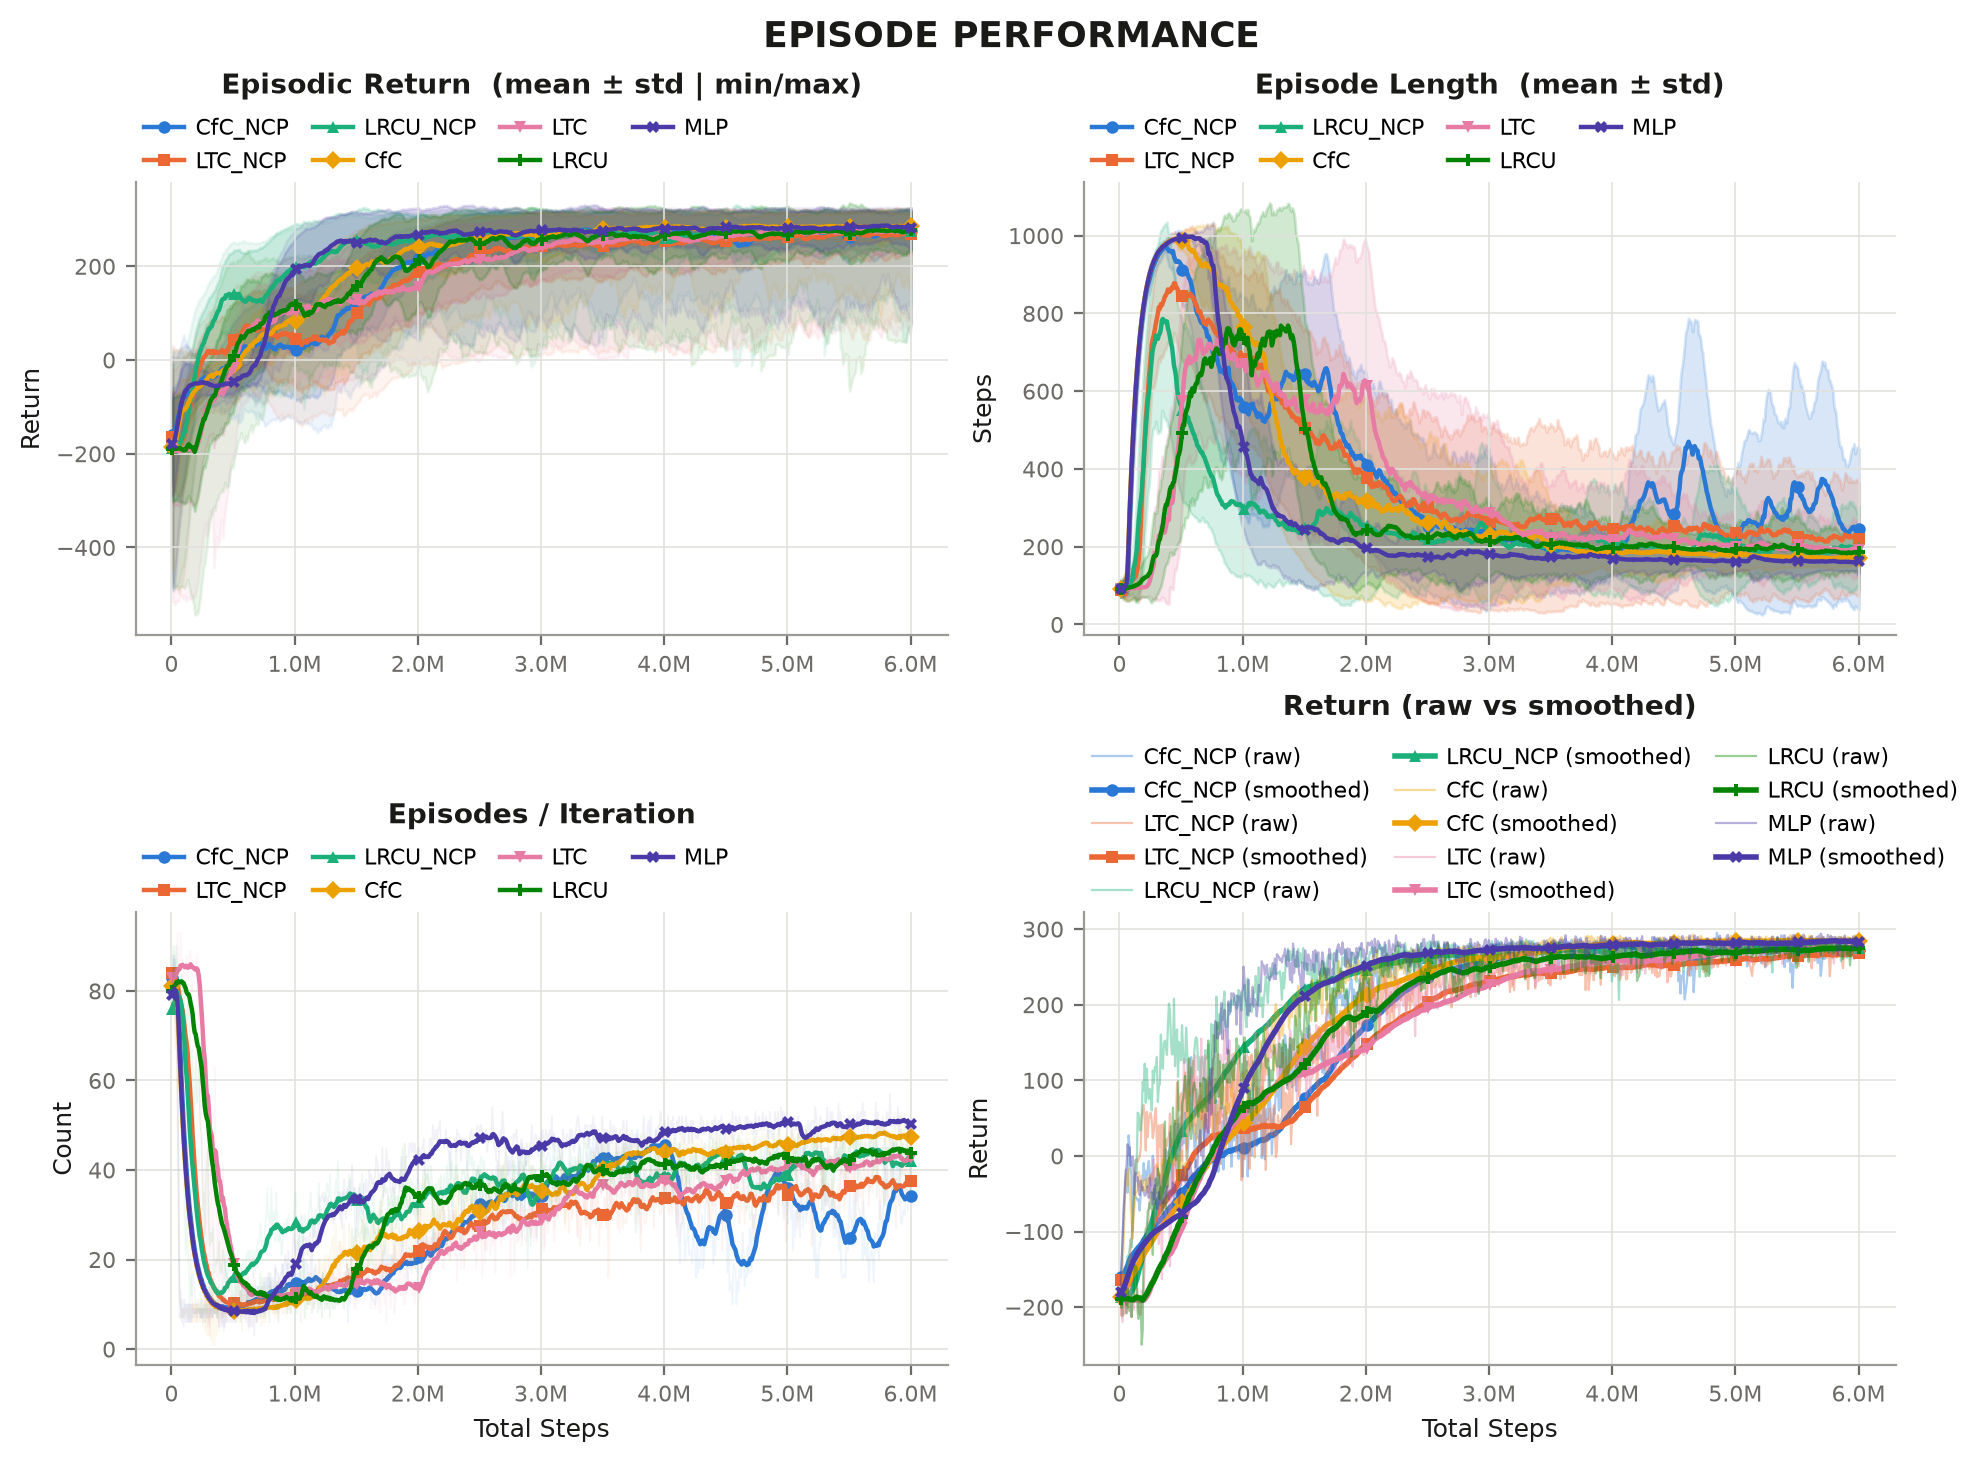
\includegraphics[width=\textwidth]{ch08/lunar_performance.png}
  \caption{LunarLander: episodic return (mean, standard deviation, minimum and
  maximum), episode length, episodes per iteration, and raw and smoothed
  return, for the seven vector networks.}
  \label{fig:res-lunar}
\end{figure}

\paragraph{Correctness of the recurrent machinery.}
The task verifies above all what a return curve does not show. The
\met{replay_logratio_max} indicator, which compares the action probabilities
recomputed by replaying the recurrent state with those recorded during
collection and must be zero up to numerical error, never exceeds
$3\cdot10^{-5}$ in any iteration of any session: the state is reconstructed
correctly at update time. The explained variance of the critic ends between
$0.93$ and $0.97$; the early stop on the KL divergence fires in fewer than 2\%
of the iterations, and never in the last fifty, because the policy step has
shrunk to a divergence of the order of $10^{-3}$. The entropy falls from
$\ln 4 \approx 1.39$, the uniform distribution over the four actions, to
$0.34$--$0.55$.

\paragraph{Speed and cost.}
The control reaches $250$ first and ties with the best network on the final
return. This is expected: the LunarLander observation contains the full state of
the vehicle, so the test verifies the \emph{machinery} --- that the recurrent
networks learn as much as a network with no need to remember --- and not the
value of memory. Among the recurrent networks the \met{LNN_LRCU_NCP} is the
fastest to reach $200$, level with the control, and the two LTC networks are the
slowest, the \met{LNN_LTC_NCP} reaching $250$ only after $3.7$ million steps.
In wall-clock time the order reverses, because here there is no encoder to
dominate the cost and the cells weigh: for the same number of steps the control
takes $22$ minutes, the CfC networks $45$--$49$, the LTC networks $54$--$63$ and
the LRCU networks $73$--$90$. The \met{LNN_LRCU_NCP} is thus the most
sample-efficient network and the least time-efficient one. The only late
anomaly is the \met{LNN_CfC_NCP}'s: between $4.2$ and $5.8$ million steps part
of its episodes go back to hovering before landing, and the mean length over
the last fifty iterations ($286$ steps) still bears its trace.

\paragraph{State norms.}
The sharpest difference between the cells is not in the return but in the state
(Figure~\ref{fig:res-lunar-states}). For CfC and LTC the largest state norm
stays below $6$ throughout the session; for the two LRCU networks it reaches
$300$--$390$. It is the growth already glimpsed on the sine wave, amplified by
episodes twenty times longer. It does not prevent learning --- the two LRCU
networks end at $276$ --- but it coincides with the only two cases of disastrous
episodes at the end of the session (worst return $-314$ and $-144$ over the last
fifty iterations, against non-negative values for CfC and the control), and it
is a signal to be watched on the fleet, where episodes are longer and the time
interval is not constant. The stability of LTC is instead the result of a
correction made on this very environment: with the hyperbolic tangent as
activation the fused step of Equation~\eqref{eq:ltc-fused} is not stable for
negative values of $f$, and an earlier session had driven the state norm to
$3\cdot10^{11}$ within \num{41} iterations. With the sigmoid, which is the original formulation
(Section~\ref{sec:cell-ltc}), $f$ is non-negative and the state stays bounded.

\begin{figure}[htbp]
  \centering
  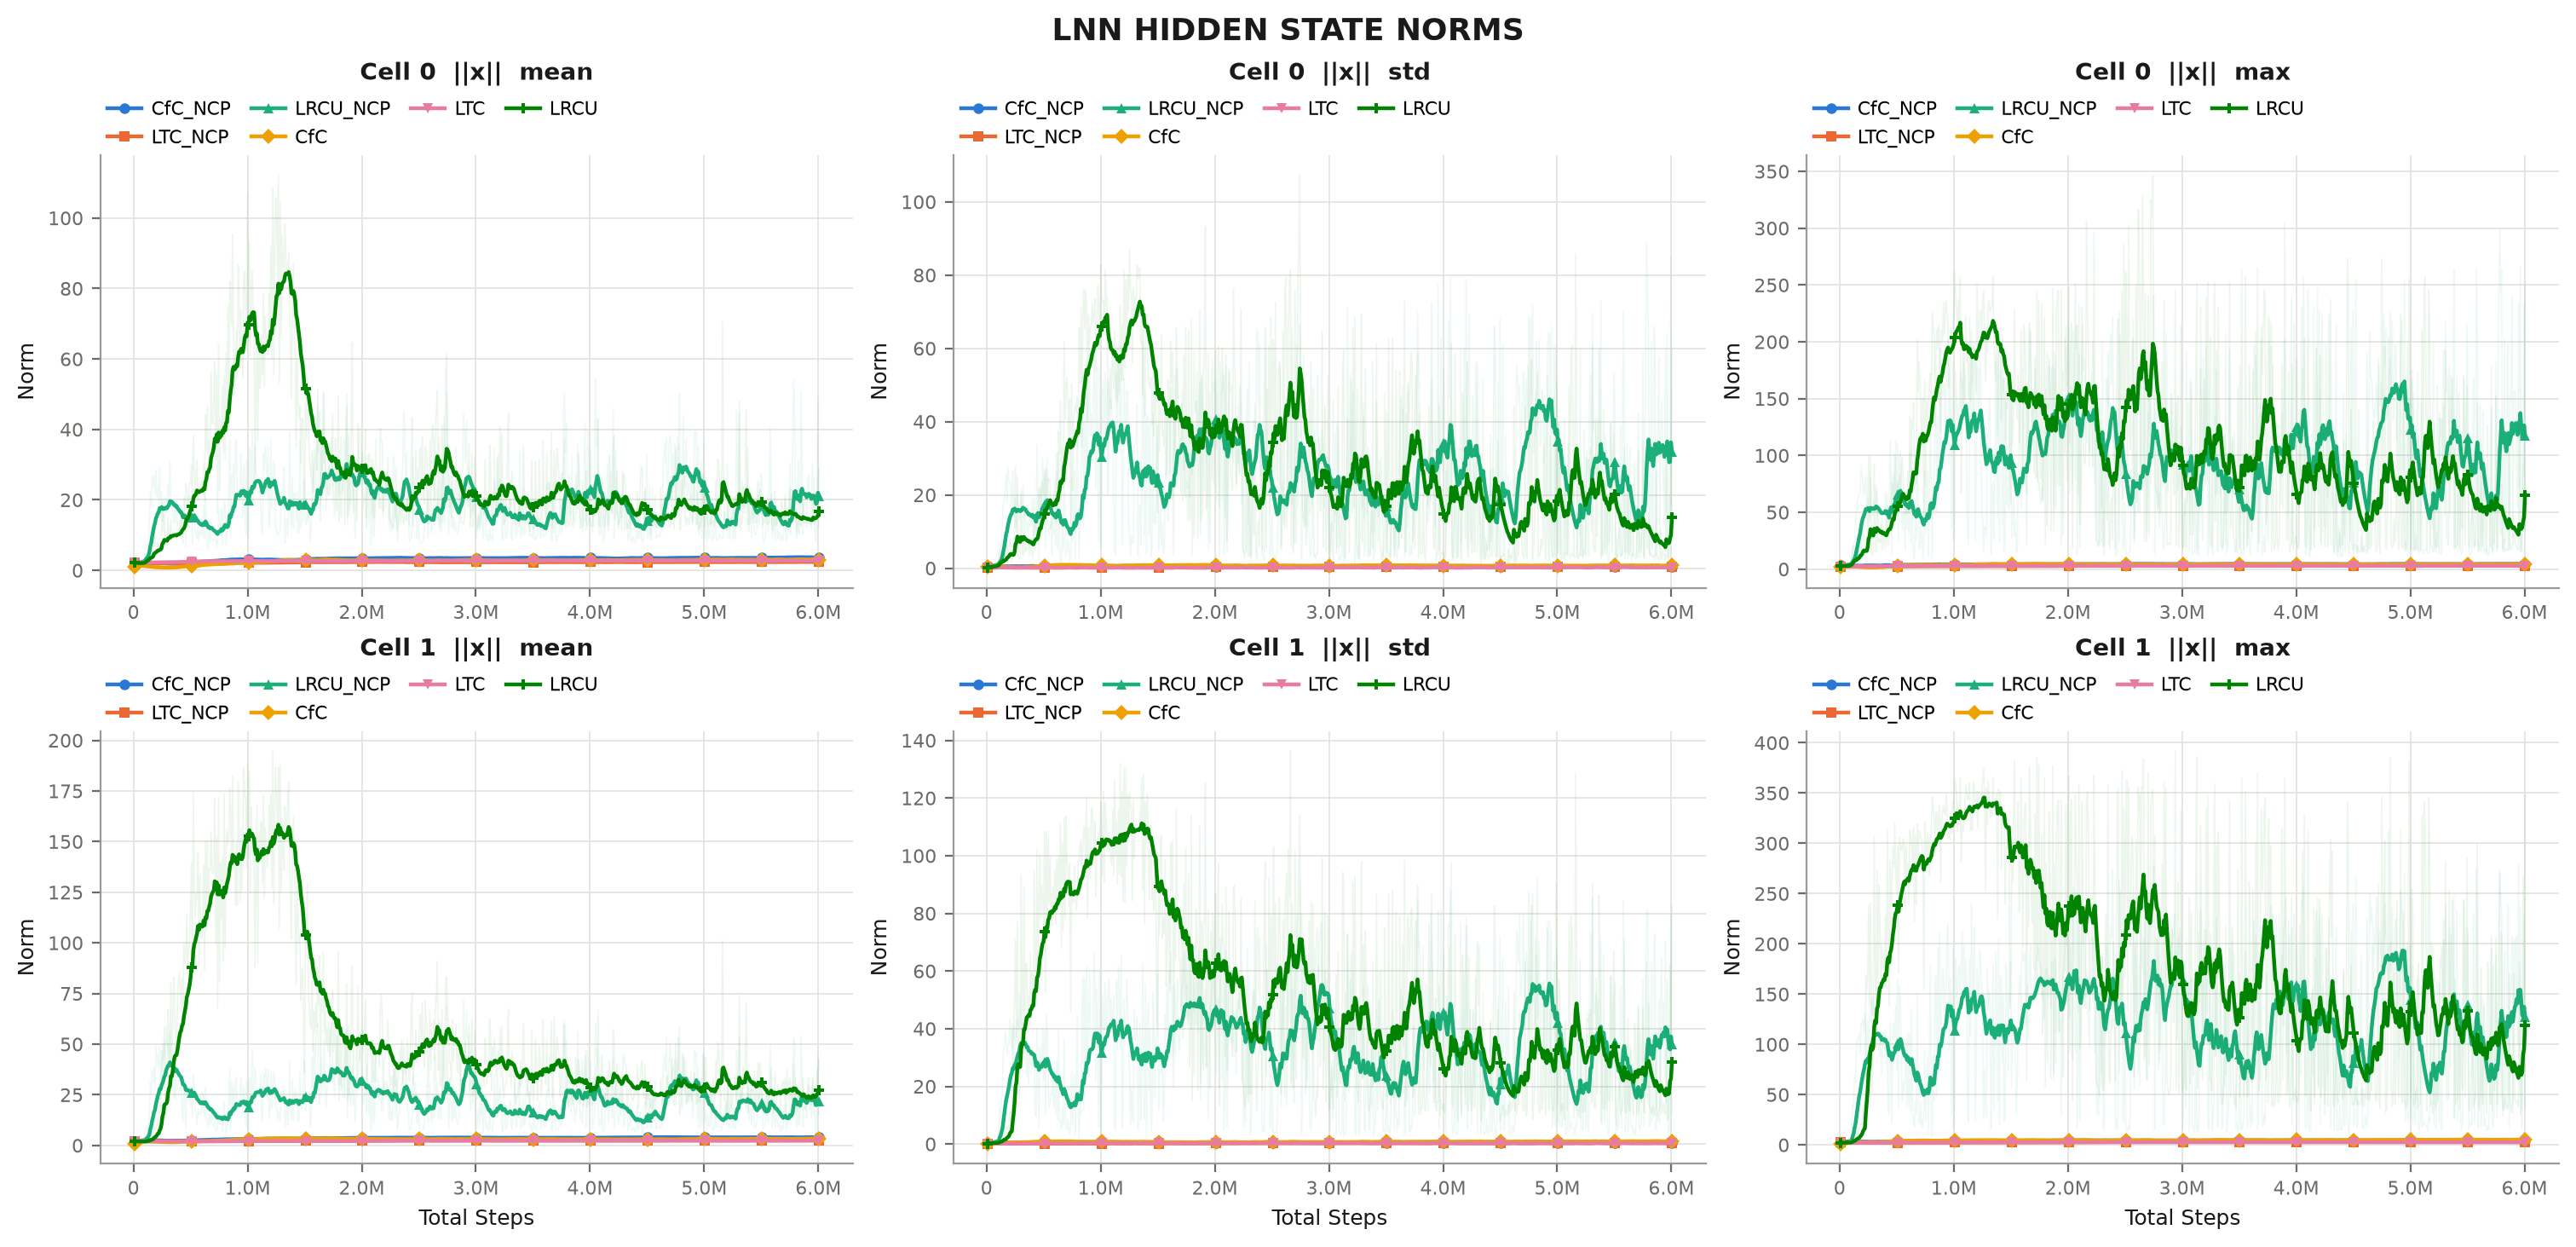
\includegraphics[width=\textwidth]{ch08/lunar_states.png}
  \caption{LunarLander: recurrent state norms per cell, for the six recurrent
  networks.}
  \label{fig:res-lunar-states}
\end{figure}

\paragraph{What the test does not verify.}
The action space is discrete, so the Gaussian policy, its learnt width and the
envelope penalty (Section~\ref{sec:rl-actions}) are not exercised; the time step
is constant; and the networks start from scratch, so the critic warm-up is not
exercised either (Section~\ref{sec:exp-protocol}). The test establishes that
the recurrent algorithm is correct and that each cell learns within it.


\subsection{Training on the Fleet}
\label{sec:res-rl-fleet}
% Sources: ~/WorkEnv/ai/tests/rl/cur_*_01/training_log.csv (7 runs, 320
% iterations each); figures from ~/WorkEnv/ai/plots/rl/cur_all/ copied to
% images/ch08/fleet_* (fleet_outcomes.png regenerated for the thesis).
% "Imitated" = iterations 1-19 (critic warm-up, actor frozen); "final" = last
% 50 iterations (271-320). Shares are per episode, each iteration weighted by
% the number of episodes that closed in it.

\paragraph{Setting.}
The seven spatial networks were fine-tuned on the fleet, each starting from its
own imitation checkpoint, the one selected in
Section~\ref{sec:res-sl-comparison}. Every session lasts \num{320} iterations
of \num{2048} transitions, that is \num{655360} environment steps, about a
ninth of the LunarLander budget; the first \num{19} iterations are reserved for
the critic (Section~\ref{sec:rl-finetuning}), and for their whole duration the
actor stays frozen bit for bit.

\paragraph{A fleet of graded difficulty.}
The fleet counts eight slices, the number the workstation of
Section~\ref{sec:exp-tooling} holds beside the training session: the slices
and the session share its \SI{16}{\gibi\byte} of accelerator memory, and with
a trainable encoder the session needs a large share of it, so that the size of
the fleet was set by the machine rather than by the throughput. The eight are
four multirotors and four rovers, all in the
\texttt{warehouse\_small} world --- a $40\times24$\,m warehouse --- and all on
the $143^3$ grid, with \SI{0.1}{\metre} voxels and a map radius of
\SI{7}{\metre}: the same grid on which Section~\ref{sec:res-sl-encoder} measures
the ablation and the probe. The slices do not pose the same task. Each platform
has four levels of difficulty, each assigned to one slice for the whole session
(Table~\ref{tab:res-fleet-slices}): a short trip with the goal ahead, one of the
same length with the goal to the side, one of \SI{5.5}{\metre} and one of
\SI{7}{\metre}, on the last two of which the straight route is clear only in
part of the episodes. This is not a curriculum: the levels do not follow one
another, they all run together from the first step to the last, and the trainer
knows nothing of them. Every batch of data therefore holds easy and hard trips
in fixed proportions, on both platforms. Spawn and goal are fixed by the
configuration of each slice and are not drawn at random: every slice poses the
same trip at every episode.

\begin{table}[htbp]
  \centering
  \small
  \caption{Fleet: the eight slices, all in the \texttt{warehouse\_small} world
  on the $143^3$ grid. \emph{Clear route} is the share of episodes in which the
  straight segment from spawn to goal crosses no obstacle; spawn and goal are
  fixed per slice. \emph{Budget} is the maximum number of steps of an episode,
  and $\gamma$ the discount derived from it.}
  \label{tab:res-fleet-slices}
  \begin{tabular}{@{}clcllrr@{}}
    \toprule
    \textbf{Slice} & \textbf{Robot} & \textbf{Level} & \textbf{Trip} & \textbf{Clear route} & \textbf{Budget} & $\gamma$ \\
    \midrule
    0 & UAV & 1 & \SI{2.5}{\metre}, ahead & always & 94  & 0.9894 \\
    1 & UAV & 2 & \SI{2.5}{\metre}, at $90^\circ$ & always & 94  & 0.9894 \\
    2 & UAV & 3 & \SI{5.5}{\metre} & $45\%$ & 207 & 0.9952 \\
    3 & UAV & 4 & \SI{7}{\metre}   & $8\%$  & 263 & 0.9962 \\
    4 & UGV & 1 & \SI{2.5}{\metre}, ahead & always & 95  & 0.9895 \\
    5 & UGV & 2 & \SI{2.5}{\metre}, at $90^\circ$ & always & 95  & 0.9895 \\
    6 & UGV & 3 & \SI{5.5}{\metre} & $43\%$ & 207 & 0.9952 \\
    7 & UGV & 4 & \SI{7}{\metre}   & $0\%$  & 263 & 0.9962 \\
    \bottomrule
  \end{tabular}
\end{table}

\paragraph{Episodes, reward and optimisation.}
The budget of every episode is three times the ideal time at maximum speed
(Section~\ref{sec:rl-episodes}), and the discount is derived per slice,
$\gamma = 1 - 1/T$ (Section~\ref{sec:rl-presets}); an episode arrives within
\SI{1.0}{\metre} of the goal, ten voxels. No collision margin is armed; the
stall condition, armed on the rovers only, ends the episode after twelve
consecutive steps in which the commanded vehicle does not move. The reward is
the \texttt{safe\_progress} policy of Section~\ref{sec:rl-reward} with its
default values --- an arrival bonus of $25$, a penalty of $10$ for losing the
vehicle --- and a cruise altitude of \SI{2.2}{\metre} for the multirotors. The
encoder is trainable, without the auxiliary geometry term.

All seven networks use the same hyper-parameters: the two presets they were
taken from are identical, and when a session starts from a checkpoint the
network is rebuilt from its metadata, so that the preset fixes only the
optimisation. The learning rate is $3\cdot10^{-5}$ for the actor and
$3\cdot10^{-4}$ for the critic, the entropy bonus $0.001$, the target KL
$0.02$, with windows of eight steps and four epochs per update. These values
are meant to fine-tune without drifting away from the imitated policy, and one
effect is visible in the logs: the width of the Gaussian, which starts at 10\%
of the envelope, is trainable but moves by at most 3\% in \num{320}
iterations, and its mean stays at $0.080$ for the whole session in every
network.

Each network was trained once, with seed $0$. A session closes between
\num{5507} and \num{8048} episodes and costs about fifteen hours, at about
\num{12} steps per second for the whole fleet: a step costs a hundred to four
hundred times as much as on LunarLander, because it is a physics simulation, a
lidar rendering and a full pass through the pipeline of
Chapter~\ref{ch:pipeline}. The cost is dominated by the environment and does
not depend on the cell, and the budget of \num{320} iterations is therefore a
time constraint rather than a choice of convergence.

Consistently with Section~\ref{sec:metrics-rl}, the result is read on the share
of episodes that reach the goal and on the reasons episodes end, not on the
return: the shares are computed per episode, each iteration weighted by the
number of episodes that closed in it.

\paragraph{The imitated policy on the fleet.}
The critic warm-up iterations are the only free measurement of the imitated
policy on the fleet, and it is from them --- not from zero --- that the gain of
the fine-tuning is to be read (Section~\ref{sec:exp-protocol}). The measurement
is clear-cut: \emph{no} imitated policy flies the task. The arrival rate goes
from 0.6\% for the control to 9.4\% for the \met{SparseConv_CfC_NCP}, and the
most frequent way for an episode to end is to run out of time: between 45\%
and 76\% of the episodes end on \met{max_steps}, the rest splitting between
tipping over (9--27\%) and stalling (4--14\%). The mean progress per episode
is negative for every network, between $-0.3$ and $-1.1$\,m: on average the
vehicle ends the episode further from the goal than it started. It is the
behaviour the restart metrics of the corpus anticipated
(Section~\ref{sec:res-sl-corpus}): a policy that at departure commands 2\% of
what the pilot commanded does not depart, and uses up the time it is given.

\paragraph{Outcome.}
After \num{320} iterations all seven networks reach the goal in between 36\%
and 63\% of the episodes (Table~\ref{tab:res-fleet},
Figure~\ref{fig:res-fleet-outcomes}), that is five to a hundred times as often
as the imitated policy they started from. The mean return per episode rises
from between $-5.7$ and $-1.2$ to between $6.3$ and $10.9$, the mean episode
length falls from \num{99}--\num{121} to \num{66}--\num{112} steps, and the
mean progress turns positive, between $0.5$ and $1.2$\,m per episode.

The course is not gradual. For roughly the first hundred iterations the arrival
rate stays below 20\% for every network, and running out of time remains the
dominant end reason; between iterations $100$ and $220$ the rate rises, in
every network, at the same moment the progress term of the reward turns
positive, that is when the policy starts closing distance instead of losing it.
Afterwards the growth slows down, and at the end of the session three networks
--- \met{SparseConv_CfC}, the control and \met{SparseConv_LTC_NCP} --- still
have their moving average at its maximum: the step budget stopped the training
before the curve flattened, and two more networks reach their maximum within
the last twenty iterations. For the remaining two the best window came earlier
--- 61\% at iteration \num{219} for the \met{SparseConv_CfC_NCP} and 48\% at
iteration \num{281} for the \met{SparseConv_LRCU} --- but the comparison is read
on the final iterations for every network, as Section~\ref{sec:exp-protocol}
prescribes, and the choice of the checkpoint to deploy is left to a later
stage.

\begin{table}[htbp]
  \centering
  \small
  \caption{Fleet: arrival rate of the imitated policy (critic warm-up
  iterations) and after fine-tuning (last 50 iterations, and separately in its
  two halves of 25), end reasons over the last 50 iterations, mean return per
  episode, and largest norm of the recurrent state.}
  \label{tab:res-fleet}
  \setlength{\tabcolsep}{3.5pt}
  \begin{tabular}{@{}lrrrrrrrr@{}}
    \toprule
    & \multicolumn{3}{c}{\textbf{Arrival rate}} & \multicolumn{3}{c}{\textbf{End reason (final)}} & & \\
    \cmidrule(lr){2-4}\cmidrule(lr){5-7}
    \textbf{Network} & \textbf{Imitated} & \textbf{Final} & \textbf{Halves} & \textbf{Flipped} & \textbf{Time} & \textbf{Stalled} & \textbf{Return} & $\lVert h\rVert_{\max}$ \\
    \midrule
    \met{CfC}         & 0.078 & 0.627 & 0.61 / 0.64 & 0.09 & 0.27 & 0.02 & 10.8 & 5.0 \\
    \met{MLP} (ctrl.) & 0.006 & 0.611 & 0.57 / 0.65 & 0.11 & 0.20 & 0.08 & 10.9 & -- \\
    \met{LTC_NCP}     & 0.038 & 0.471 & 0.45 / 0.49 & 0.04 & 0.35 & 0.13 &  7.4 & 3.2 \\
    \met{CfC_NCP}     & 0.094 & 0.464 & 0.46 / 0.47 & 0.03 & 0.38 & 0.13 &  6.5 & 2.9 \\
    \met{LRCU}        & 0.069 & 0.405 & 0.43 / 0.38 & 0.06 & 0.50 & 0.03 &  6.3 & 76.8 \\
    \met{LRCU_NCP}    & 0.021 & 0.385 & 0.36 / 0.41 & 0.10 & 0.50 & 0.02 &  6.9 & 6.9 \\
    \met{LTC}         & 0.051 & 0.356 & 0.35 / 0.36 & 0.06 & 0.54 & 0.05 &  7.5 & 3.6 \\
    \bottomrule
  \end{tabular}
\end{table}

\begin{figure}[htbp]
  \centering
  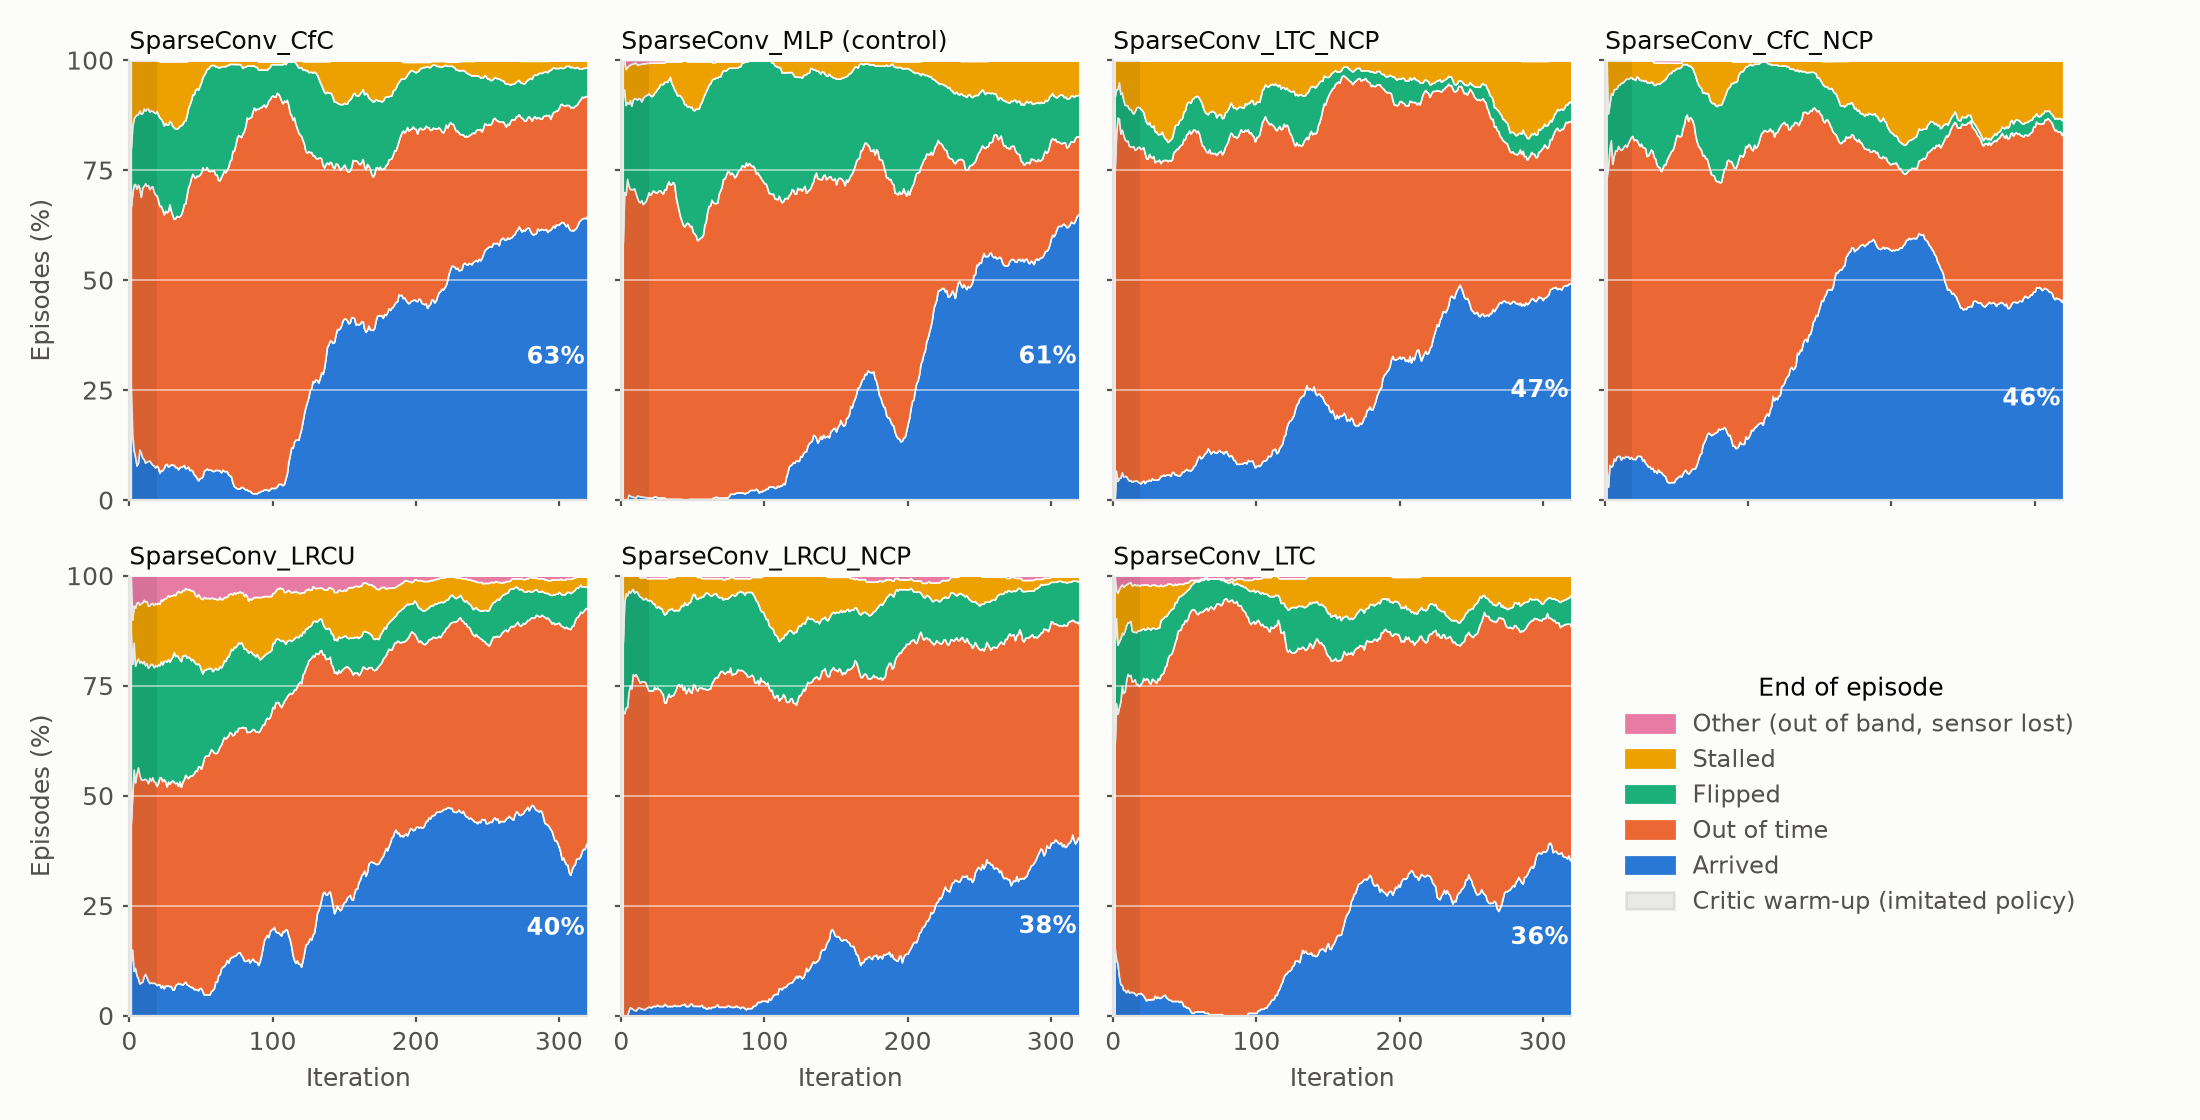
\includegraphics[width=\textwidth]{ch08/fleet_outcomes.png}
  \caption{Fleet: how episodes end over the \num{320} iterations, one panel per
  network. Shares per episode, as a moving average over 20 iterations weighted
  by the number of episodes; arrivals sit at the baseline so that they compare
  across panels. The grey band is the critic warm-up, that is the imitated
  policy; the figure in each panel is the arrival rate over the last 50
  iterations (Table~\ref{tab:res-fleet}).}
  \label{fig:res-fleet-outcomes}
\end{figure}

\paragraph{How episodes end.}
Most of the gain comes from episodes that used to end on the clock: for six
networks out of seven the share of \met{max_steps} falls by $16$--$49$ points;
for the \met{SparseConv_LRCU}, which started from the lowest share (45\%), it
rises slightly, to 50\%. Tipping over is roughly halved in every network, from
9--27\% to 3--11\%, whereas stalling moves in different directions: it falls
for four networks, stays level for the control, and rises for the two NCP
networks with the CfC and LTC cells, from 4\% to 13\% and from 11\% to 13\%.
Fine-tuning, in other words, taught above all how to \emph{depart} and arrive
in time, and secondarily how to lose the vehicle less often. Even at the end of
the session, running out of time remains the main cause of failure for every
network, between 20\% and 54\% of the episodes.

\paragraph{What the return is made of.}
The decomposition of the reward (Section~\ref{sec:metrics-rl-reward}) shows
that, at the end of the session, the mean reward per step coincides in practice
with the terminal term alone: the ratio between the two lies between $0.96$
and $1.08$ for every network. The progress earned ($+0.005$ to $+0.018$ per
step) and the dense costs --- time, fixed at $-0.0064$, safety ($-0.003$ to
$-0.005$) and altitude ($-0.0005$ to $-0.0014$) --- cancel almost exactly, and
the return is in practice a count of arrivals. This is consistent with what the
reward budget prescribes (Section~\ref{sec:rl-reward}): the dense costs must not
be able to cost more than progress gives back, and they do not. It follows,
however, that the return adds no information to the arrival rate, which is why
Table~\ref{tab:res-fleet} reports it for completeness only.

\paragraph{Optimisation.}
The critic starts from nothing and it shows: during the warm-up the explained
variance lies between $0.17$ and $0.36$, at the end of the session between
$0.88$ and $0.94$. The trust region is instead the binding constraint for
almost the whole session: after the warm-up the actor's update is stopped early
in 58--79\% of the iterations for six networks out of seven, and in 31\% for
the \met{SparseConv_LTC}. Every iteration therefore moves the policy as far as
the region allows and no further, and it is plausibly this, together with the
step budget, that sets the pace at which the arrival rate grows.

\begin{figure}[htbp]
  \centering
  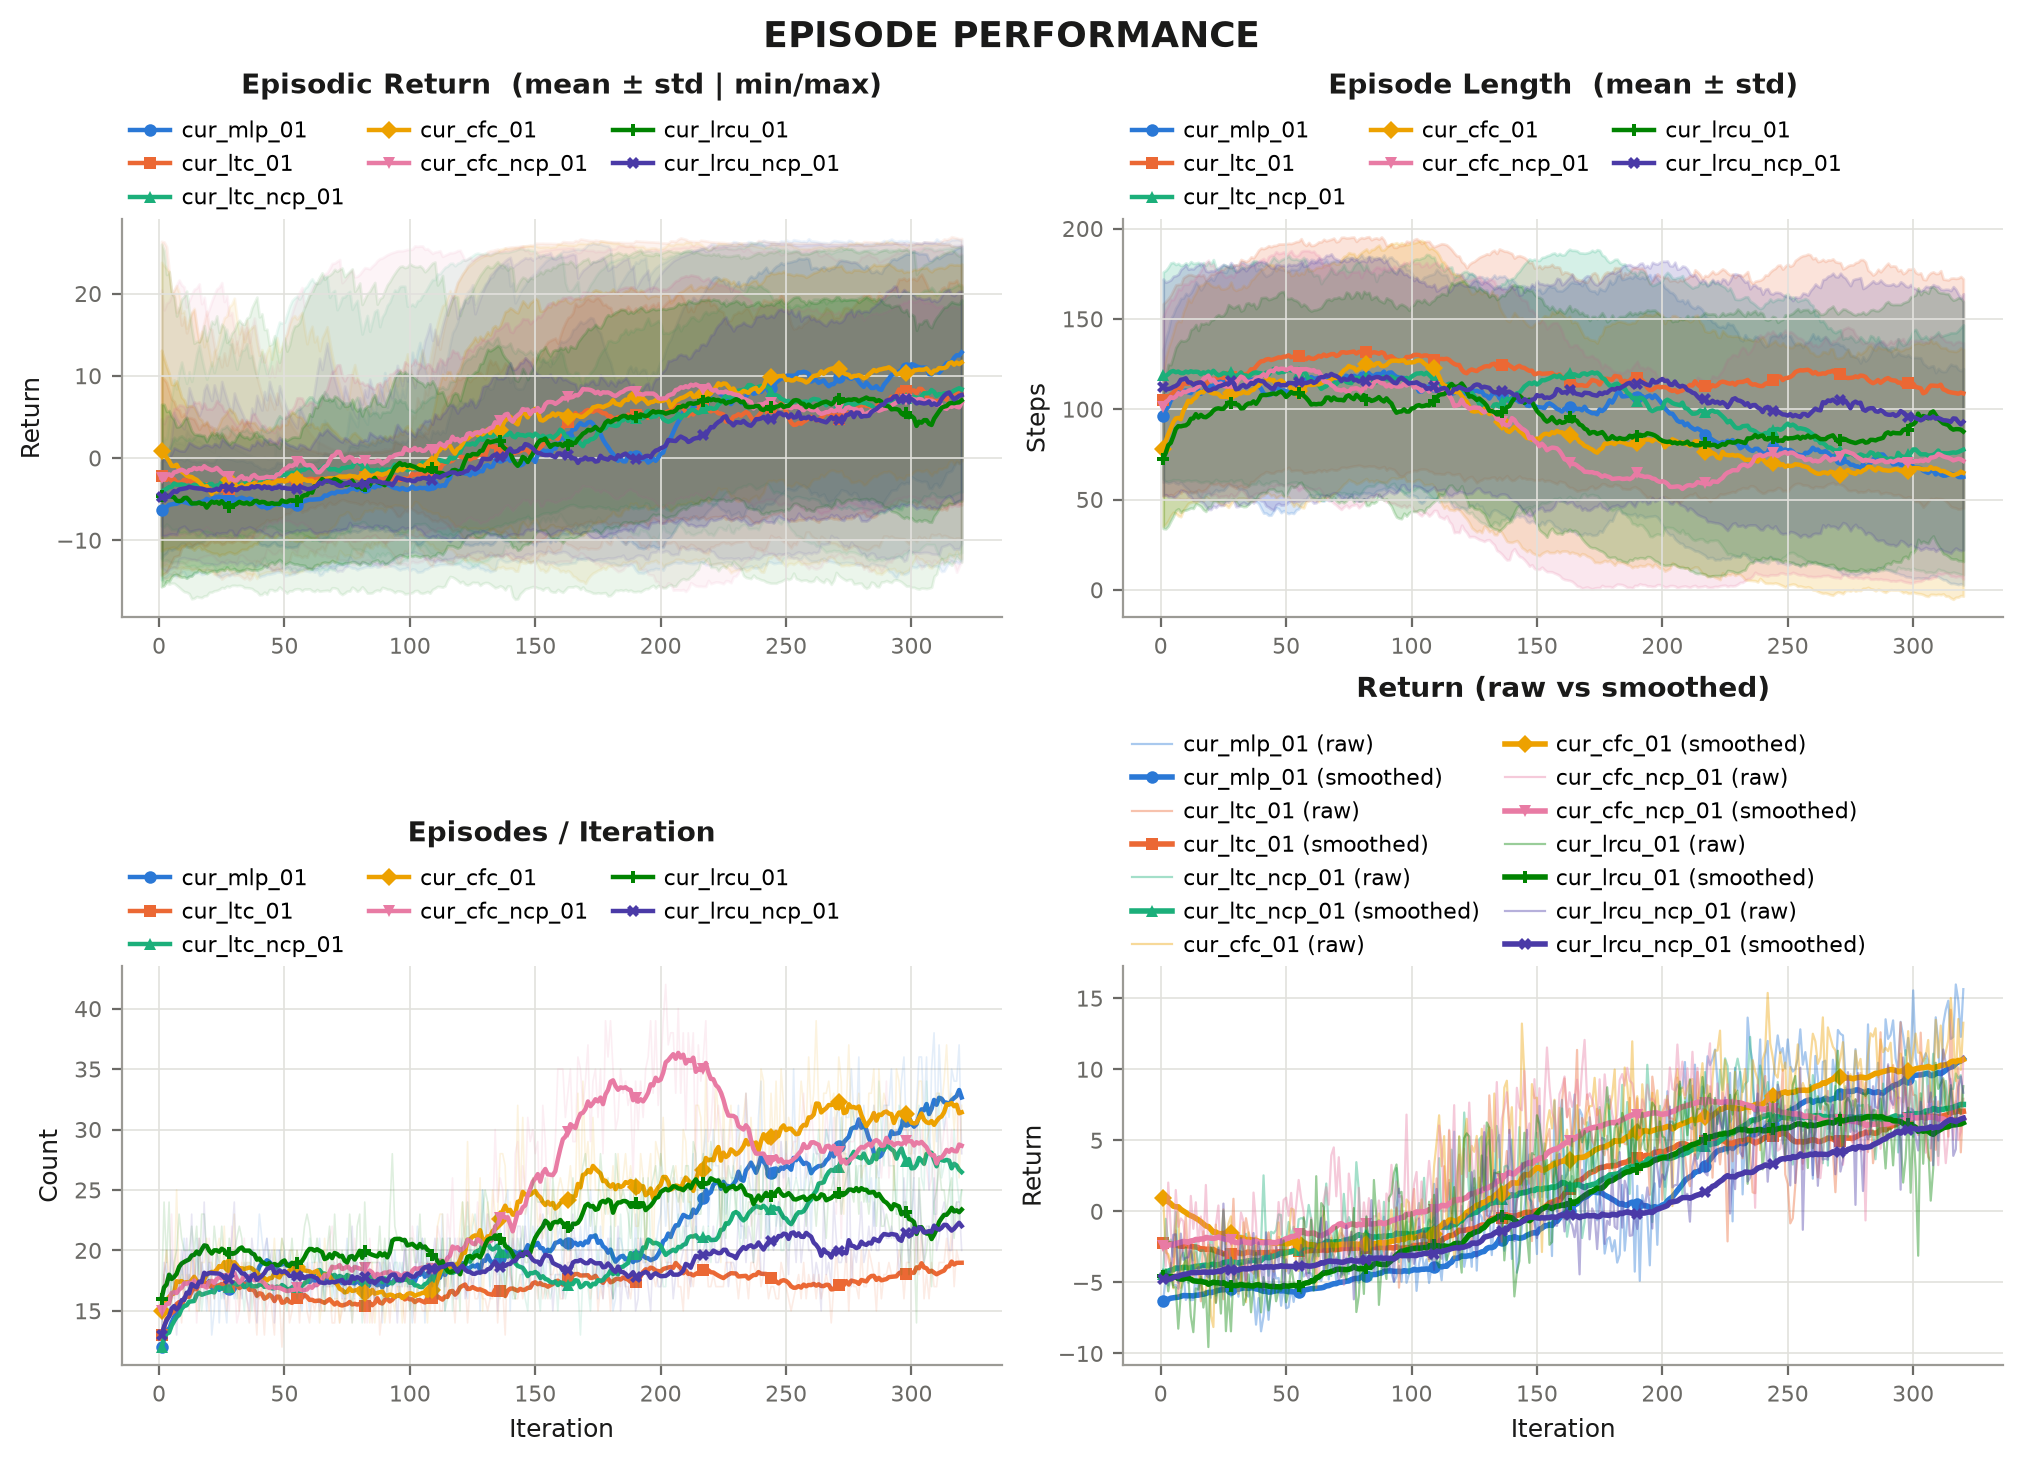
\includegraphics[width=\textwidth]{ch08/fleet_performance.png}
  \caption{Fleet: episodic return (mean, standard deviation, minimum and
  maximum), episode length, episodes per iteration, and raw and smoothed
  return, for the seven spatial networks.}
  \label{fig:res-fleet-performance}
\end{figure}

\paragraph{The preliminary sessions.}
The configuration used is the last of a series, and four measurements from the
earlier sessions explain why the result is read on the end reasons and on the
progress rather than on the return. In one session the share of episodes
ending tipped over went from 73\% to 97\% while the return improved from $-19$
to $-4.6$: the policy had learnt to lose the vehicle sooner, paying fewer dense
costs. In another, of \num{650} iterations, the mean progress per episode fell
from $1.26$ to $0.04$\,m while the return rose throughout. In both cases the
return improved while the task got worse. The other two measurements concern
the reward itself: the progress term in its canonical form, telescoped over an
episode, is worth $d(s_0)(1-\gamma^T)$, that is $+5.6$ on a slice with a short
trip and $+24.5$ on the one with the long trip, against an arrival bonus of
$20$ --- on that slice, standing still paid more than arriving --- and in a
later configuration the terminal term alone carried 90\% of the return. These
measurements are what led to the undiscounted progress term and to the double
budget constraint of Section~\ref{sec:rl-reward}.


\subsection{Architecture Comparison}
\label{sec:res-rl-comparison}

The conditions of the comparison are those of Section~\ref{sec:exp-protocol}:
the same step budget, the same fleet, the same reward, and for every network the
imitation checkpoint of the same architecture. The optimisation hyper-parameters
are also the same for all the networks.

\paragraph{Two groups, again.}
The networks split into two groups. The \met{SparseConv_CfC} and the control
arrive in 61--63\% of the episodes; the other five between 36\% and 47\%. The
separation between the two groups, about $15$ points, exceeds the oscillation
within each run: between the first and the second half of the last fifty
iterations the arrival rate of the same network changes by at most $8$ points.
Within each group, by contrast, the differences are of the same order as that
oscillation and are not to be read as a ranking. With a single run per network,
and with a fleet whose interleaving across slices depends on the load of the
machine (Section~\ref{sec:exp-protocol}), even the separation between the two
groups remains indicative rather than established.

\paragraph{The stateless control.}
The network without memory arrives as often as the best recurrent one, although
it started from the worst imitated policy of all (0.6\%), and although on the
fleet the task is partially observable: the cloud sees only within the map
radius and the velocity is estimated. What this implies for the comparison is
discussed in Section~\ref{sec:res-discussion}.

\paragraph{Wiring and cells.}
The NCP wiring, which on the corpus improved the loss for the same cell, brings
no consistent advantage on the fleet: the \met{SparseConv_CfC} beats its NCP
variant ($0.63$ against $0.46$), the \met{SparseConv_LTC_NCP} beats the
\met{SparseConv_LTC} ($0.47$ against $0.36$), and the two LRCU networks are
equivalent ($0.41$ and $0.39$). The \met{SparseConv_CfC_NCP} also shows the
largest late regression: its moving average reaches 61\% at iteration \num{219}
and falls back to 46\% by the end, while the episode length and the number of
episodes per iteration follow the same course
(Figure~\ref{fig:res-fleet-performance}). Without a second run it cannot be
said whether this is an instability of the network or an oscillation of the
session.

The LRCU cells confirm on the fleet what the sine wave and LunarLander had
shown. The largest state norm of the \met{SparseConv_LRCU} is $72$--$77$
throughout the session, against $3$--$7$ for all the others
(Figure~\ref{fig:res-fleet-states}); the NCP variant stays below $7$. It is the
only network whose arrival rate drops between the two final halves (43\% and
38\%). The LRCU networks are also those whose imitated policy most often
commands outside the envelope: during the warm-up the mean of the Gaussian of
the \met{SparseConv_LRCU_NCP} falls outside the limits in 16.5\% of the steps
and that of the \met{SparseConv_LRCU} in 13.2\%, against less than 1\% for the
others; fine-tuning brings both below 5\%.

\begin{figure}[htbp]
  \centering
  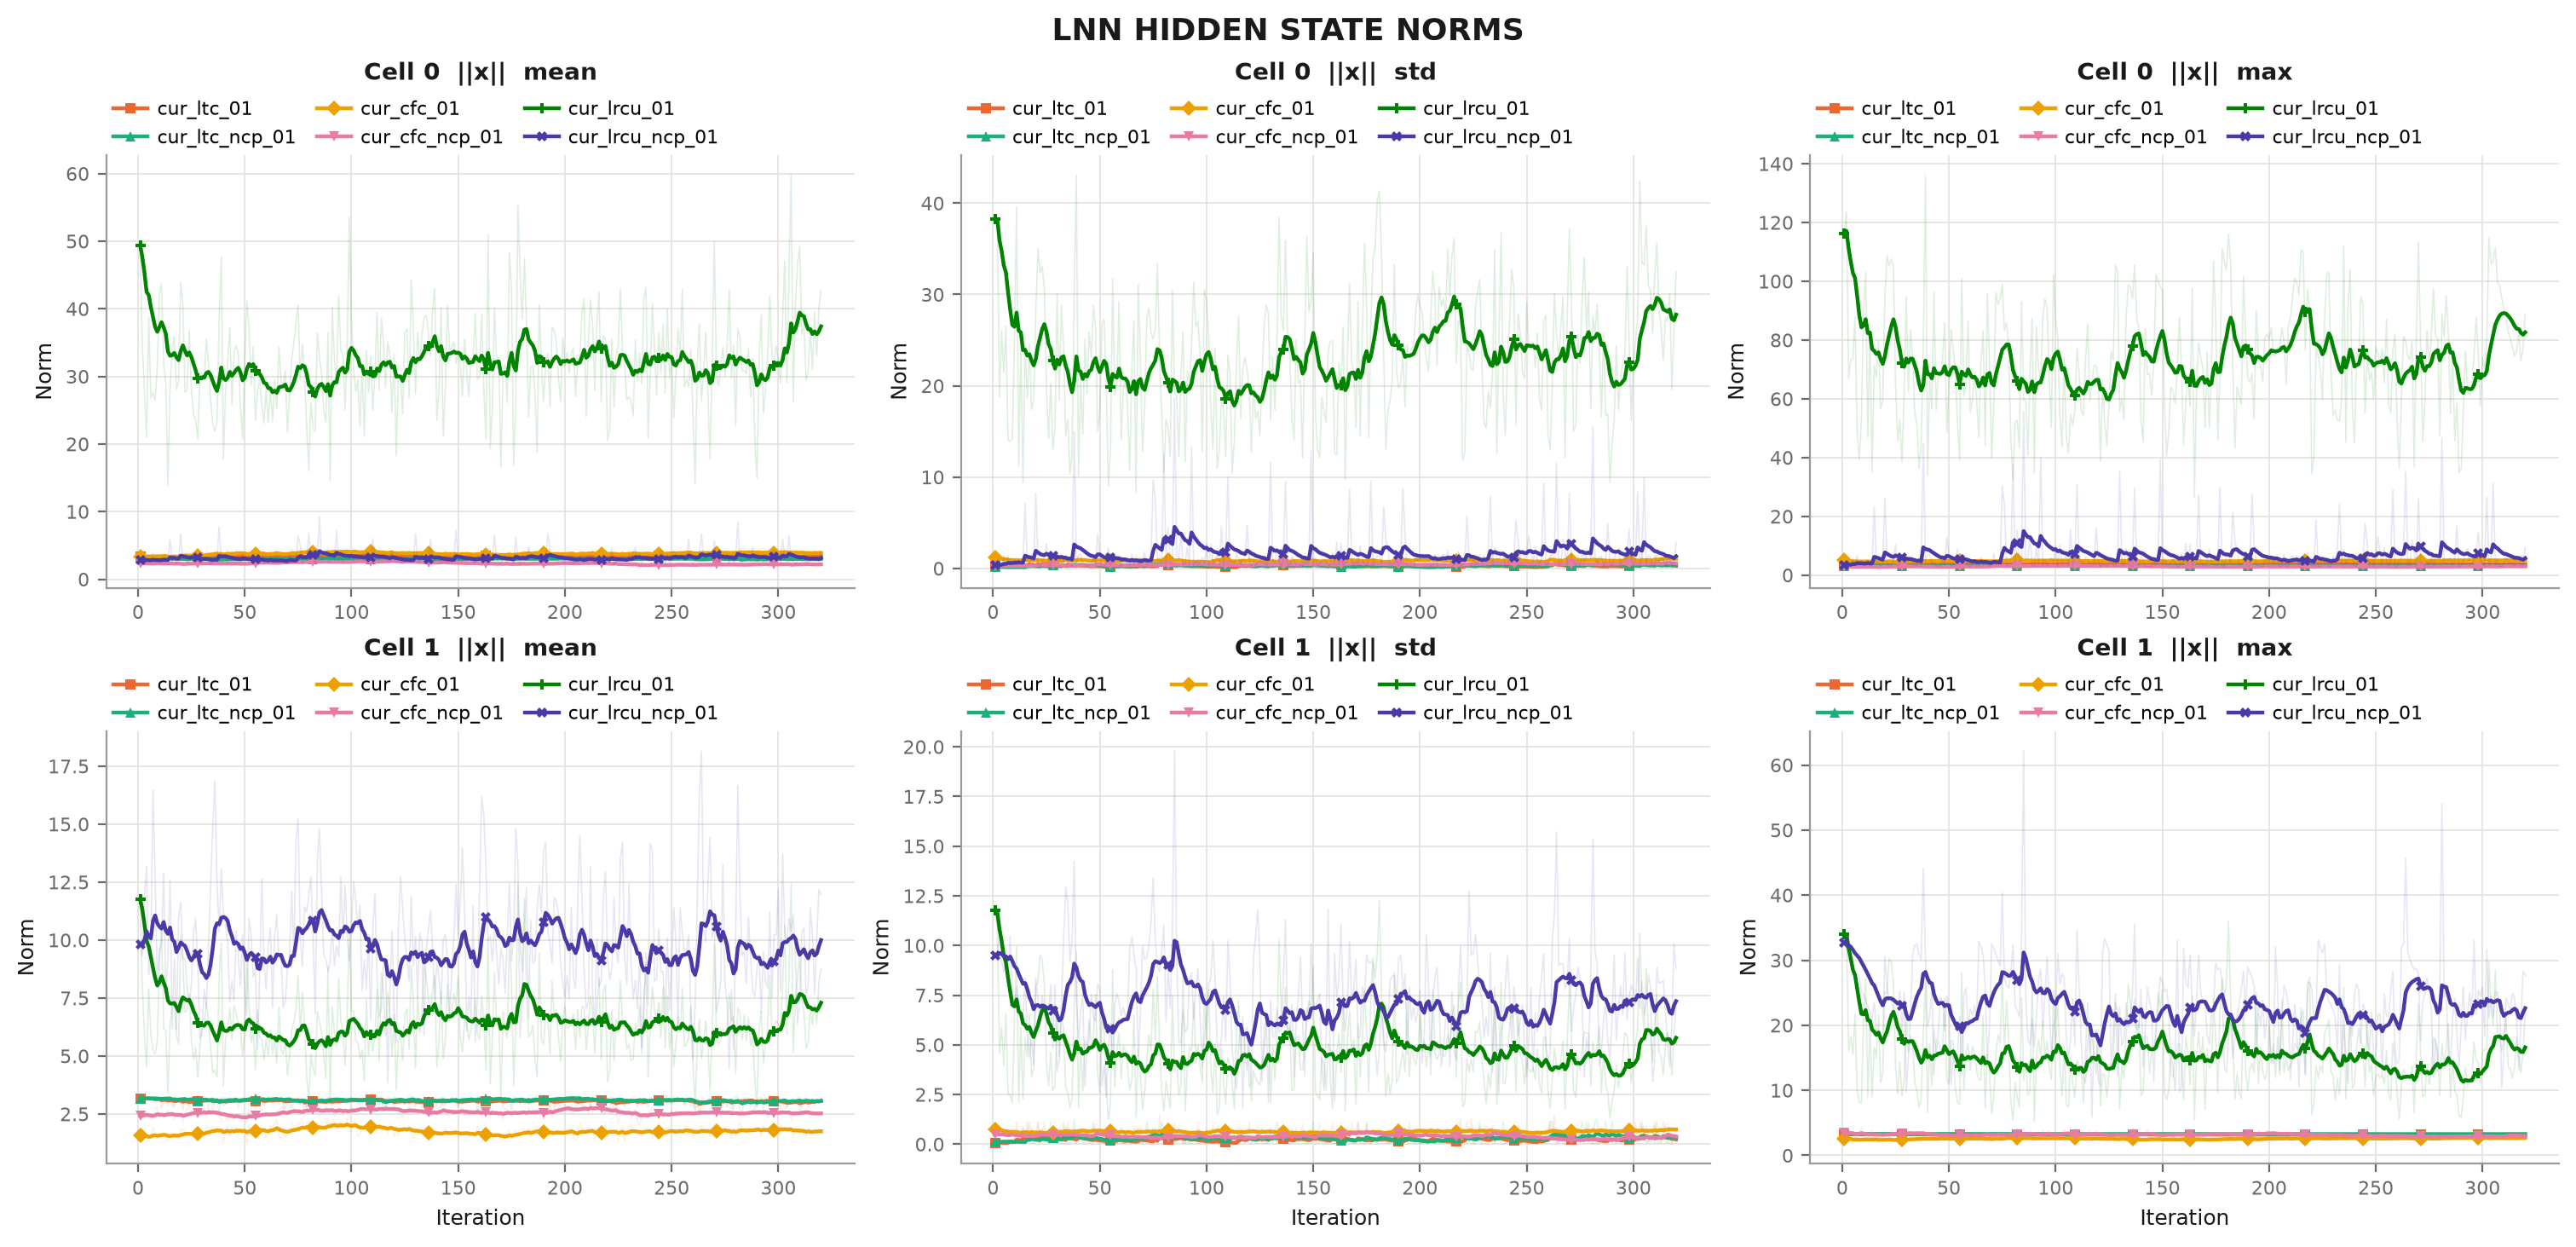
\includegraphics[width=\textwidth]{ch08/fleet_states.png}
  \caption{Fleet: recurrent state norms per cell, for the six recurrent
  networks.}
  \label{fig:res-fleet-states}
\end{figure}


\section{Cross-Stage Analysis}
\label{sec:res-cross}

The two stages were evaluated separately; this section asks what the first says
about the second. The sample is seven networks, one run each: with seven points
a rank correlation is significant at the 5\% level only beyond
$|\rho| \approx 0.79$, and what follows is to be read against that threshold.

\paragraph{The imitation loss does not predict how the imitated policy flies.}
The ranking of the networks by test loss (Table~\ref{tab:res-test}) and the
ranking by arrival rate of the imitated policy on the fleet are unrelated
($\rho = -0.14$). The extreme case is the control: second by loss, last by
arrivals (0.6\%). This is not surprising: the mean loss is dominated by the
moving frames and by the forward velocity, whereas what decides whether an
episode arrives is the departure --- the rare event on which every imitated
network fails in the same way (Section~\ref{sec:res-sl-corpus}). The loss
measures well what it measures, and that is not what the fleet needs.

\paragraph{The quality of the imitation weakly predicts the end point.}
The ranking by loss is, on the other hand, related to the \emph{final} arrival
rate ($\rho = -0.64$) and to the gain of the fine-tuning ($\rho = -0.75$): the
three networks with the lowest loss are three of the four with the best final
result, and the CfC-plus-control group is the same in the two stages. Neither
coefficient clears the threshold, and the two groups also coincide with the
speed of convergence observed on the corpus, so that the quality of the
starting point cannot be separated from how easily the network optimises.

\paragraph{How much the network uses the map predicts the gain.}
The strongest relation is with the encoder ablation (Table~\ref{tab:res-encoder}):
how much the validation loss degrades when the information of the cloud is
removed is related to the final arrival rate and to the gain of the fine-tuning
($\rho = +0.79$ for both, at the threshold). The networks whose imitated command
depends most on the map are those that fine-tuning takes furthest. The probe,
by contrast, is related to neither ($|\rho| \le 0.32$, on the $143^3$ grid
alone as well): that the descriptor \emph{contains} the geometry predicts
nothing; that the command \emph{uses} it does. This is the most useful
indication for future work, because it suggests selecting the imitation
checkpoint on its dependence on the map as well, and not on the loss alone.

\paragraph{What fine-tuning corrected.}
Read together with Section~\ref{sec:res-sl-corpus}, the result on the fleet
matches point by point the main defect of the imitation. The corpus showed a
policy that at a restart commands 2\% of what the pilot commanded; the fleet
shows imitated policies that run out of time in 45--76\% of the episodes with
negative progress; fine-tuning removes up to fifty points from that end reason
and moves almost all of them to arrivals. What fine-tuning corrected only in
part is just as readable: tipping over is halved, but stalls --- contact with
an obstacle for the vehicles that do not fly --- do not fall consistently, and
they rise precisely for two of the networks that arrive best. This is
consistent with what the probe found on the fleet's grid: the directional
distance to the obstacles is the part of the scene the encoder represents
worst.


\section{Discussion, Limitations and Threats to Validity}
\label{sec:res-discussion}

\paragraph{What the results establish.}
The whole chain works: the three cells learn a known dynamics, the recurrent
agent is correct and learns on a reference problem, the imitation of the corpus
generalises to unseen episodes with an error a third of that of echoing the
velocity, and fine-tuning on the fleet takes the arrival rate from below 10\% to
between 36\% and 63\% for every architecture. The two-stage procedure therefore
produces a policy that flies a task imitation alone does not.

\paragraph{What they do not establish.}
The comparison between architectures does not single out a winner, and the
reason is the control. In all three stages the network without state is among
the best: second by loss on the corpus, the fastest on LunarLander, level with
the best recurrent network on the fleet. In each case the difference between
the control and the best recurrent network is smaller than the variability
within a single run, so that on the tasks used memory has not shown that it is
worth its state.

The three stages say this for different reasons. On LunarLander it is expected,
because the observation contains the full state of the vehicle. On the corpus
the observation already carries the robot's velocity, the position of the goal
and, through the encoder, the local geometry, so that the part of the command
imitation can learn is largely a function of the current state; and where the
demonstration is ambiguous --- the restart --- no network, with or without state,
reaches $10\%$ of what the pilot commanded. On the fleet the task is partially
observable, and the control still arrives as often as the best recurrent
network. The hypothesis that continuous-time cells bring an advantage on this
problem is therefore not refuted, but it is not supported by the data either.

\paragraph{Threats to internal validity.}
\begin{itemize}
  \item \emph{One run per configuration.} Each network was trained once per
        stage. The rule of Section~\ref{sec:exp-protocol} asks for the spread
        across seeds to be measured before a difference is stated; here it was
        replaced by the oscillation within a run (across epochs, across halves of
        a window), which underestimates it. All differences between
        architectures are therefore reported as indicative.
  \item \emph{Fixed budgets.} Twenty epochs on the corpus and \num{320}
        iterations on the fleet are time constraints. On the corpus LTC and LRCU
        were still descending at the last epoch; on the fleet three networks were
        still at their maximum. The comparison measures in part the speed of
        convergence.
  \item \emph{Asynchrony of the fleet.} Two identical runs do not collect the
        same sequence of transitions; the seed fixes the tasks and not their
        order.
  \item \emph{Shared hyper-parameters.} The networks use the same optimisation
        configuration, tuned on the \met{SparseConv_CfC_NCP}; it may suit some
        cells better than others.
  \item \emph{Fleet-level metrics.} Arrival rates and end reasons are recorded
        over the whole fleet, not per slice: multirotors and rovers cannot be
        separated, nor can the four levels. A difference between architectures
        concentrated on the hard trips may therefore be diluted by the easy
        ones.
\end{itemize}

\paragraph{Threats to external validity.}
\begin{itemize}
  \item \emph{Simulation only.} No policy has been run on a real robot. The
        observation pipeline is the same as on board
        (Section~\ref{sec:rl-environment}), but the dynamics, the sensors and
        the latencies are those of the simulator.
  \item \emph{One world, four fixed levels.} Fine-tuning took place in a single
        world and on trips between \SI{2.5}{\metre} and \SI{7}{\metre}; nothing
        says how the policy behaves on more cluttered maps or on longer trips.
  \item \emph{A small, unbalanced corpus.} \num{476} episodes, two robots, two
        worlds; 86\% of the energy of the command on a single component, the
        lateral velocity absent. The probe finds the directional geometry poorly
        readable precisely on the fleet's grid, which limits what imitation can
        transfer.
  \item \emph{Validation used twice.} The validation partition selected the
        epoch and fitted the calibration; the test partition, read once, shows
        that this introduced no appreciable bias (Table~\ref{tab:res-test}).
\end{itemize}


%!TEX root = ../main.tex
\chapter{Conclusions}
\label{ch:conclusions}

\section{Summary of the Work}
\label{sec:conclusions-summary}

\section{Future Work}
\label{sec:conclusions-future}


% ----- APPENDICES -----
\begin{appendices}
%!TEX root = ../main.tex
\chapter{Metric Reference}
\label{app:metrics}

This appendix defines, column by column, the metrics summarised in
Chapter~\ref{ch:experiments}. It is meant to be consulted rather than read: each
entry names the column as it appears in the log file, states what it measures,
and where the choice is not obvious, why it is computed the way it is.

\section{Supervised Training Metrics}
\label{app:metrics-supervised}

\subsection{Reference Predictors and Skill Scores}
\label{sec:metrics-r2}

A loss value on its own has no scale: \num{0.01} may be excellent or useless
depending on how large the commands are. The trainer therefore evaluates two
zero-parameter reference predictors on every batch and expresses the model's
error relative to them.

\paragraph{The zero predictor.}
\met{baseline_zero_loss} is Equation~\eqref{eq:capscaled} evaluated with
$\hat{\mathbf{y}} = \mathbf{0}$: the loss of a model that always commands
``hold still''. A run whose loss sits at or below this line has learnt nothing
beyond predicting nothing, which is the signature of the most common failure
mode observed---a loss that drops once in the first epoch and never moves
again.

The same comparison is made per component, with a plain (unscaled) squared
error so that the yardstick does not depend on the choice of loss:
%
\begin{equation}
  \text{\met{mse_dim_i}} = \frac{1}{N}\sum_{n}(\hat{y}_{n,i} - y_{n,i})^{2},
  \qquad
  \text{\met{baseline_dim_i}} = \frac{1}{N}\sum_{n} y_{n,i}^{2},
\end{equation}
%
and their ratio gives a coefficient of determination against the zero
predictor,
%
\begin{equation}
  \text{\met{r2_dim_i}} = 1 - \frac{\text{\met{mse_dim_i}}}{\text{\met{baseline_dim_i}}}.
  \label{eq:r2}
\end{equation}
%
A value of $1$ is a perfect fit, $0$ means the model is no better than
predicting zero, and a negative value means it is worse. The reason for
reporting this \emph{per dimension} is that the target energy of this corpus is
heavily concentrated in a single component of the six
(Section~\ref{sec:res-sl-corpus}), so an aggregate error that improves says
almost nothing about the other five; a model can score well overall while having
learnt only the dominant one.

Two details of the computation matter. The ratio in
Equation~\eqref{eq:r2} is formed \emph{once per epoch} from the two epoch
means, not per batch and then averaged, because the pooled $R^2$ is a ratio of
means and not a mean of ratios. And when \met{baseline_dim_i} is exactly zero
the split never commands that component; the ratio is undefined, the column is
omitted rather than filled with an infinity, and the raw \met{mse_dim_i} is
kept, where it reads as pure error.

\paragraph{The persistence predictor.}
The observation already contains the robot's current linear and angular
velocity, which is the same physical quantity as the command one step later
and strongly correlated with it. Echoing that velocity is therefore a
zero-parameter rule that is far harder to beat than silence, and a model that
does not beat it is not worth its parameters. The loader exposes this echo as
$\mathbf{p}_n$ (masked to zero on the components the robot cannot reach or the
corpus never commands), and the trainer logs
%
\begin{equation}
  \text{\met{persist_dim_i}} = \frac{1}{N}\sum_{n}(p_{n,i} - y_{n,i})^{2},
  \qquad
  \text{\met{skill_dim_i}} = 1 - \frac{\text{\met{mse_dim_i}}}{\text{\met{persist_dim_i}}},
\end{equation}
%
together with \met{persist_loss}, the cap-scaled loss of the echo itself.
The \emph{skill score} is positive only when the model earns its parameters.
It is the stricter of the two ratios: a run can show a comfortable
\met{r2_dim_i} and a negative \met{skill_dim_i} at the same time, which means
it has learnt to reproduce the current velocity and little else.

\subsection{Amplitude and Restart Ratio}
\label{sec:metrics-amplitude}

A squared error cannot see one failure that matters a great deal for a
deployed controller. A model trained by least squares regresses towards the
conditional mean of the demonstration: where the pilot sometimes commanded a
strong manoeuvre and sometimes none, the model learns to command a weak one
every time. This is not a bug of the optimiser---it is what minimising
squared error does under uncertainty---but a robot flown by such a model is
sluggish, and the squared error \emph{rewards} the behaviour rather than
exposing it. Two metrics exist to expose it.

\paragraph{Amplitude ratio.}
The trainer logs the first and second moments of both prediction and target
per component (\met{sq_pred_dim_i} $= \mathbb{E}[\hat{y}_i^{2}]$,
\met{mean_pred_dim_i} $= \mathbb{E}[\hat{y}_i]$ and
\met{mean_true_dim_i} $= \mathbb{E}[y_i]$; the second moment of the target is
\met{baseline_dim_i}) and forms, once per epoch,
%
\begin{equation}
  \text{\met{amplitude_dim_i}}
  = \sqrt{\frac{\operatorname{Var}(\hat{y}_i)}{\operatorname{Var}(y_i)}}
  = \sqrt{\frac{\mathbb{E}[\hat{y}_i^{2}] - \mathbb{E}[\hat{y}_i]^{2}}
               {\mathbb{E}[y_i^{2}] - \mathbb{E}[y_i]^{2}}}.
\end{equation}
%
A value of one means the model reproduces the spread of the demonstrated
commands; a value well below one means it returns something closer to their
average than to any of them. The variance rather than the raw second moment
is used because on a component with a large mean the second moment is
dominated by that mean, and the spread---which is what collapses when a head
averages two modes---barely moves it.

\paragraph{Restart ratio.}
The frames that decide whether a deployed policy ever leaves standstill are
those in which the robot is at rest and the demonstration starts moving. They
are a fraction of the corpus small enough to be invisible in any aggregate, so
they are isolated explicitly. A frame is a \emph{restart frame} when the
measured velocity is below \SI{0.02}{} on every component and the demonstrated
command exceeds \SI{0.05}{} on at least one (in each component's own units).
Over those frames the trainer logs their count, \met{restart_frames}, and
%
\begin{gather}
  \text{\met{restart_pred_dim_i}} = \mathbb{E}\!\left[\hat{y}_i \cdot \operatorname{sign}(y_i)\right],
  \qquad
  \text{\met{restart_true_dim_i}} = \mathbb{E}\!\left[\,|y_i|\,\right],
  \\
  \text{\met{restart_ratio_dim_i}} = \frac{\text{\met{restart_pred_dim_i}}}{\text{\met{restart_true_dim_i}}}.
\end{gather}
%
The prediction is projected onto the demonstrated direction rather than taken
in absolute value: an absolute value would count noise around zero as if it
were a command and read high for a model that never moves. A restart ratio
near one means the model commands the departure the pilot commanded; near zero
it means the model would leave the robot sitting at its spawn. As with the
other ratios, the two halves are logged separately and divided once per epoch.

\subsection{Still and Moving Frames}
\label{sec:metrics-still}

A substantial share of the samples in the corpus are all-zero commands
(Section~\ref{sec:res-sl-corpus}). These are legitimate ``hold still'' targets---the pilot waiting, hovering, or
paused---and not missing labels, but they are also the easiest samples to
score well on. \met{mse_still} and \met{mse_moving} split the plain squared
error by whether the target is exactly zero on every component, so that it is
possible to tell how much of a score comes from recognising a stop and how
much from reproducing a manoeuvre. A model that scores well overall but poorly
on \met{mse_moving} is scoring on the stops.

Both columns are emitted for every batch, as \emph{not a number} when the
batch contains no frame of that kind; the epoch average is then taken only
over the batches in which the quantity was defined, so that the reported
value means what its name says.

\subsection{Per-Robot Breakdown}
\label{sec:metrics-per-robot}

The corpus is recorded on more than one platform, and a drone and a ground
robot do not use the same command components: vertical velocity is not merely
rare for a ground robot, it is unreachable. A fleet average can therefore
hide one robot being served well and another badly. Whenever the batch
carries robot identifiers, every per-dimension pair is repeated per model as
\met{mse_m<id>_dim_i} and \met{baseline_m<id>_dim_i}, and the logger derives
\met{r2_m<id>_dim_i} from them with no further bookkeeping. How many models a
batch holds follows from how it was filled: the sparse convolution takes one
grid per call, so a batch is built out of windows that share a grid, and a
validation batch is one episode and therefore one robot, while a training
batch may draw from several episodes at once and hold more than one. The
per-model averages are taken only over the batches in which that model
appears.

\subsection{Calibrated Metrics}
\label{sec:metrics-calibrated}

The output calibration of Section~\ref{sec:output-calibration}, fitted
according to the protocol of Section~\ref{sec:sl-calibration}, corrects the
regression to the mean before deployment. It is the per-component affine map
%
\begin{equation}
  \tilde{y}_i = g_i\,\hat{y}_i + b_i,
  \qquad
  g_i = \frac{\operatorname{Cov}(\hat{y}_i, y_i)}{\operatorname{Var}(\hat{y}_i)},
  \qquad
  b_i = \mathbb{E}[y_i] - g_i\,\mathbb{E}[\hat{y}_i],
\end{equation}
%
which is the least-squares regression of the demonstrated command on the
model's prediction, refitted on the validation split once per epoch. Since the
policy that flies is the calibrated one, the columns below report what the robot
would execute rather than what the optimiser sees, and a component on
which either side carries no signal is left switched off ($g_i = b_i = 0$),
since a demonstration that never commands it has nothing to fit.

Because the calibrated output is what the robot is actually given, the whole
family of validation metrics is computed a second time through the fitted
calibration and logged with the prefix \met{val_cal_}: \met{val_cal_loss},
\met{val_cal_r2_dim_i}, \met{val_cal_amplitude_dim_i},
\met{val_cal_restart_ratio_dim_i}, and so on. The uncalibrated
\met{val_} family describes a model that is never deployed; the
\met{val_cal_} family describes the one that is.

The calibrated numbers are mildly optimistic, since the correction was fitted
on the same frames it is scored on. It is two parameters per component
against a whole split, so the optimism is small, but it is the reason
\met{val_loss}---fitted to nothing---remains the quantity that ranks
checkpoints.

\subsection{Auxiliary Geometry}
\label{sec:metrics-geometry}

The auxiliary head of Section~\ref{sec:geometry-head}, supervised as described
in Section~\ref{sec:sl-geometry}, contributes its own columns. One property of
the headline number belongs here: \met{train_loss} and \met{val_loss} remain the
imitation loss alone, so a run with the head and a run without it are still
ranked on the same quantity. Whether the head changes the policy is a question
for Chapter~\ref{ch:results}.

The auxiliary error itself is \met{geometry_loss}, a squared error over the
entries the cloud could measure, expressed in fractions of the map radius.
The scaling is what puts frames recorded on grids of different extent on one
scale, and it is also what makes a sector holding nothing read the same value
everywhere. An entry the measurement could not fill is left out of the loss
rather than counted as zero, since zero clearance is not a missing value but a
collision, and would be learnt as one.

The skill score is formed as the others are, from means logged separately and
divided once per epoch, and is reported for two groups: $i = 0$ for the sector
clearances pooled and $i = 1$ for the height. From \met{geometry_mse_dim_i},
\met{geometry_sq_true_dim_i} and \met{geometry_mean_true_dim_i},
%
\begin{equation}
  \text{\met{geometry_explained_dim_i}}
  = 1 - \frac{\text{\met{geometry_mse_dim_i}}}
             {\mathbb{E}[y_i^{2}] - \mathbb{E}[y_i]^{2}},
\end{equation}
%
the fraction of the geometry's spread the head accounts for, where $0$ is a
head that predicts the average clearance and nothing more. Two choices in that
denominator are deliberate. It is the spread over the \emph{epoch} and not
within a batch, because a validation batch is a single episode and one robot's
height above the ground barely varies inside it, so a per-batch variance would
divide by almost nothing. And it is the spread rather than the second moment
used in Equation~\eqref{eq:r2}, because these targets are distances and not
commands centred on zero: the zero predictor, which is the reference the
$R^2$ of that equation is built on, is not a meaningful one for them.

\met{grad/geometry_head} is the head's gradient norm, logged beside the
network's own \met{grad/encoder}. It is separate because the head is trained
with the network but lives outside it, so it is not one of the sub-modules
\met{grad/<module>} enumerates.

\subsection{Model Health}
\label{sec:metrics-health}

The metrics above describe the output. A further group describes whether the
parts of the network that produce it are doing anything, which no loss curve
reveals.

\paragraph{Encoder spread.}
The architectures that consume a point cloud pass it through a sparse
convolutional encoder that reduces tens of thousands of voxels to a
200-dimensional descriptor (Section~\ref{sec:sparse-encoder}). \met{encoder/mean} and
\met{encoder/norm} are the mean value and the mean Euclidean norm of that
descriptor over the batch, and \met{encoder/std} is its standard deviation
\emph{across the samples of the batch}, per feature, averaged over features.
A value near zero means the encoder answers nearly the same vector whatever
cloud it is shown: the sparse branch is contributing nothing, the policy is
effectively flying on odometry alone, and the loss curve shows nothing of it.

The across-sample form is the only one that can detect this. The encoder ends
with a layer normalisation that pins every single descriptor to zero mean and
unit deviation across its channels, so a spread measured \emph{inside} one
descriptor reads $1.0$ whatever the input and the check could never fire.
That same normalisation is why the across-sample value has no absolute scale
to be read against: the descriptor's own magnitude is fixed, so the column
answers ``is this encoder answering differently to different clouds'' and not
``by how much'', and it is read as a comparison---against the checkpoint a run
started from, or against the same architecture untrained---rather than against
a threshold. When a batch holds a single sample the column is omitted, because
$0.0$ would read as the failure rather than as the absence of a measurement.

\paragraph{Hidden-state norms.}
For every recurrent cell $k$ in the network, \met{state/cell_<k>/mean},
\met{state/cell_<k>/std} and \met{state/cell_<k>/max} are the mean,
standard deviation and maximum over the batch of the Euclidean norm of the
cell's hidden state after the forward pass. They catch the two ways a
recurrent state goes wrong: growth without bound, and collapse to zero.

\paragraph{Gradient norms.}
\met{grad/total} is the global $L_2$ norm of the gradient before clipping,
the most immediate signal that training has stalled, and it is the one extra
number printed on the console at every epoch. \met{grad/<module>} is the same
norm restricted to each top-level sub-module of the network (the encoder, the
input layer, each cell, the output head), which is where a dead branch shows
up: a module absent from the list received no gradient at all in that batch,
which is not the same as receiving a small one, and the distinction separates
an unused branch from a merely quiet one. Gradient norms exist only for the
training split, since evaluation has no backward pass.

\paragraph{Cost.}
\met{epoch_time_s} is the wall-clock duration of the epoch, which together
with the number of parameters and the number of samples gives the throughput
of each architecture.


\section{Reinforcement Learning Metrics}
\label{app:metrics-rl}

\subsection{Task Performance}
\label{sec:metrics-rl-task}

\paragraph{Episodic return and length.}
For every episode that closed during the iteration, the trainer records the
undiscounted sum of the environment's rewards and the number of steps. They
are reported as \met{ep_return_mean}, \met{ep_return_std},
\met{ep_return_min}, \met{ep_return_max}, \met{ep_length_mean} and
\met{ep_length_std}, together with \met{n_episodes}, the number of episodes
those statistics average, and \met{episodes_total}, the running count since
the start of the run. The distinction between the last two matters:
\met{n_episodes} at zero says that nothing closed \emph{just now}, which is
normal on a fleet whose episodes last a thousand steps, whereas
\met{episodes_total} at zero says that nothing has \emph{ever} closed, which
is a fault. The return is computed from the environment's own reward, before
the truncation bootstrap described in Section~\ref{sec:rppo-gae} is added:
that bootstrap is right for the advantage trace and wrong for a reported
return, which would otherwise move with the critic on every truncated step.

\paragraph{Success rate and end reasons.}
The return alone cannot tell an episode that arrived from one that crashed.
Every episode ends for a named reason, and the trainer reports the fraction
of the iteration's closed episodes that ended for each as \met{term/<reason>}.
On the fleet the reasons are \texttt{goal} (arrived within tolerance),
\texttt{collision}, \texttt{flipped} (attitude beyond the terminal angle),
\met{out_of_band} (left the altitude envelope), \met{stalled} (commanded to
move and did not, for a run of consecutive steps), \met{sensor_lost} (the
lidar returned nothing for two consecutive steps) and \met{max_steps}
(the time budget expired). \met{success_rate} is the share of the first.
\met{stalled} reaches a collision through its consequence rather than through
a clearance, and it is armed only on the slices that do not fly, where an
impact does not announce itself by tipping the vehicle over; on a fleet of
flying slices the column simply never appears.
The set of columns is counted rather than declared: whatever the environment
names becomes a column, so a fleet that adds a terminal condition gets a
column without the trainer changing. A blank cell therefore means ``did not
occur'' when episodes closed and ``not measured'' when none did, and the
plotting code reads the shares against \met{n_episodes} for that reason.

Why this is the primary metric, and not the return, follows from the structure
of the reward: with a dense progress term and a fixed crash penalty, ``get
closer, then crash'' scores better than ``crash early'' and keeps improving for
as long as the agent gets further, so the return can rise for a whole run while
the task is never solved. A run of this work in which exactly that happened is
reported in Section~\ref{sec:res-rl-fleet}.

\paragraph{Progress closed per episode.}
\met{ep_progress_mean} and \met{ep_progress_std} are the metres closed
between an episode's first observation and its last, measured as the
difference in distance to the goal. The column exists because the return can
disagree with it, and when they disagree it is the return that misleads. The
progress term of the reward is a potential-based shaping
\cite{ng1999policy} whose discounted sum over an episode telescopes to
$d(s_0) - \gamma^{T} d(s_T)$; the second half does not vanish at a terminal,
so an episode that ends far from the goal still collects
$d(s_0)\,(1 - \gamma^{T})$, which on a long slice is a sizeable fraction of the
arrival bonus itself. A run whose episodes all truncate therefore shows a
comfortably positive return while nothing has been achieved, and
Section~\ref{sec:res-rl-fleet} reports one in which this column fell towards
zero while the return improved throughout. It is absent, rather than zero, on an
environment that reports no distance.

\paragraph{Episodes in flight.}
Three columns describe the episodes that are \emph{still running} at the end
of the rollout: \met{inflight_steps}, the age of the oldest open episode;
\met{inflight_budget}, the mean step budget of the open episodes as the
environment sized them; and \met{inflight_d_goal}, their mean current distance
to the goal. Without them a run in which nothing has finished yet reports
\emph{not a number} for every episodic column and nothing else, and a long
episode cannot be told from one that can never end. \met{inflight_budget} is a
mean over the open episodes, so a fleet whose budgets are fixed reports one
value for the whole run however different its slices are: it says how long an
episode is allowed to be, and nothing about how varied the fleet is.

\subsection{Policy Optimisation Diagnostics}
\label{sec:metrics-rl-policy}

PPO improves the policy by maximising a clipped surrogate objective over
several passes on the same rollout. The quantities below are computed on every
mini-batch of the update and averaged over the iteration, except where
stated; in the recurrent case only the real, non-padded positions of a
sequence contribute.

\paragraph{Losses.}
\met{pg_loss} is the clipped policy-gradient surrogate,
$-\mathbb{E}[\min(r_t A_t,\ \operatorname{clip}(r_t, 1-\epsilon, 1+\epsilon)\,A_t)]$
with $r_t = \pi_\theta(a_t \mid s_t)/\pi_{\theta_{\text{old}}}(a_t \mid s_t)$
the probability ratio, where the advantages are normalised to zero mean and
unit variance within each mini-batch so that the step size does not depend on
the reward's scale. \met{entropy} is the mean entropy of the action
distribution, and \met{actor_loss} is the total actor objective,
$\text{\met{pg_loss}} - c_{\text{ent}}\cdot\text{\met{entropy}}$.

\paragraph{Approximate KL divergence and the trust region.}
\met{approx_kl} is the estimated Kullback--Leibler divergence between the
policy that collected the rollout and the one being updated, using the
low-variance estimator $\mathbb{E}[(r_t - 1) - \log r_t]$. It is the
quantity that decides when the update stops: after every mini-batch the
running mean of the estimate over the current epoch is compared to
\met{target_kl}, and when it exceeds the threshold the actor stops for the
rest of the update, since the data no longer describes the current policy.
\met{kl_early_stop} records whether that happened (0 or 1) and
\met{epochs_run} how many of the \met{n_epochs} passes the actor completed.
Zero there is ambiguous on its own and is read beside \met{critic_warmup}
below, which is the other way an iteration can run no actor epoch at all.
The critic keeps fitting either way, as it has no ratio and nothing to be
wrong about.

The estimator is heavy-tailed on the small mini-batches a recurrent update
uses---sixteen samples on the fleet's preset---so a single sample above the
threshold is more often an outlier than a movement. The stop therefore acts
on the epoch's running mean, read only once it has at least eight informative
estimates, and only mini-batches scored \emph{after} the first optimiser step
count as informative (before it, the ratio is exactly one and the estimate
exactly zero). \met{approx_kl_max} is the largest per-mini-batch estimate of
the iteration, the one series a mean would destroy. It is read beside
\met{approx_kl}: close together, the policy genuinely steps that far and the
levers are \met{target_kl} or the learning rate; far apart, the estimator is
noisy and the mini-batch is too small.

\paragraph{Clip fraction.}
\met{clip_frac} is the fraction of samples whose ratio left the interval
$[1-\epsilon, 1+\epsilon]$, i.e.\ the share of the batch that hit the hinge of
the surrogate. Near zero the policy is barely moving---steps too small, or
advantages near zero; very high, it is being pushed hard against the hinge on
every batch. \met{clip_eps} is the value of $\epsilon$ in effect, logged
because it is annealed over the run.

\paragraph{Replay consistency.}
\met{replay_logratio_max} is a correctness check specific to the recurrent
implementation. On the first mini-batch of the first epoch, before anything
has been optimised, the update's forward pass should reproduce the rollout's
log-probabilities exactly, so the log-ratio must be zero to floating-point
error (about $10^{-6}$). A larger value means the update's forward pass is not
the rollout's---almost always a hidden state that was restored incorrectly---
and its only other symptom is a \met{clip_frac} that reads like an aggressive
learning rate. Cheap to compute and included for that reason
\cite{engstrom2020implementation}.

\paragraph{Optimisation state.}
\met{lr_actor} and \met{lr_critic} are the two learning rates in effect,
logged separately because the actor and the critic have separate optimisers
and separate annealing. \met{actor_grad_norm} is the actor's gradient norm
before clipping, averaged over the optimiser steps actually taken (it is
undefined on mini-batches the early stop skipped, and those are excluded from
the mean rather than dragging it to zero).

\paragraph{Critic warm-up.}
\met{critic_warmup} is $1$ on the iterations in which only the critic is
learning. A run that starts from imitated weights arrives with a policy worth
keeping and a critic that knows nothing about it, so the first advantages
measure the critic's error rather than the action's merit; those iterations
spend them on the critic alone. The column exists because every actor-side
number is then flat for a reason that has nothing to do with the policy: the
actor's weights, its exploration width and the auxiliary head are left
untouched, and \met{epochs_run} reads $0$. It marks, too, the only iterations
in which the task metrics of Section~\ref{sec:metrics-rl-task} describe the
imitated weights exactly as they were handed over, since nothing has yet moved
them.

\subsection{Value Function}
\label{sec:metrics-rl-value}

The critic estimates $V(s)$, and everything in the advantage rests on it. Its
health is described by the following columns.

\paragraph{Losses.}
\met{vf_loss} is the mean squared regression error of $V(s)$ onto the GAE
returns, optionally clipped so that the value cannot move more than a fixed
range from what it predicted during collection; \met{critic_loss} is the same
quantity times its coefficient. \met{critic_grad_norm} is the critic's
gradient norm before clipping.

\paragraph{Explained variance.}
The single most informative number about the critic is
%
\begin{equation}
  \text{\met{explained_var}}
  = 1 - \frac{\operatorname{Var}(R_t - V(s_t))}{\operatorname{Var}(R_t)},
\end{equation}
%
computed over the \emph{whole rollout}, with the values the rollout was
collected with. A value of $1$ is a perfect critic, $0$ one no better than
predicting the mean return, negative one worse than that.
\met{explained_var_batch} asks the same question of each mini-batch and
averages the answers, and it is logged beside the first only as a warning: a
mini-batch is a handful of sequences of \emph{consecutive} steps whose returns
barely vary, so its denominator is tiny and individual batches reach large
negative values that the mean inherits. Measured on a fleet run,
\met{explained_var_batch} sat near $-1.4$ for 390 iterations with a minimum of
$-58$, while the value estimate tracked the returns in mean and spread
throughout. The per-batch figure had already been acted on---the discount had
been cut on its evidence---before the discrepancy was understood, which is why
the rollout-level one is the number the diagnostic tables in
Chapter~\ref{ch:results} are calibrated against.

\paragraph{Value and return statistics.}
\met{value_mean}, \met{value_std}, \met{value_min} and \met{value_max}
describe the distribution of $V(s)$ over the update, and \met{return_mean}
and \met{return_std} that of the GAE returns it is regressed onto;
\met{value_mse} is their mean squared difference. \met{value_std} deserves
its own reading: exactly $0.0$ is not a small number, it is a constant
predictor. During this work a whole fleet run reported \met{value_std}
exactly $0.0$ and \met{explained_var} of $10^{-6}$ because the critic
received the observation on a different scale from the actor; every unit of
its first activation layer saturated, and the only thing the value head could
still learn was its output bias. The advantages were then simply the raw
returns.

\paragraph{Advantages.}
\met{adv_mean} and \met{adv_std} are the mean and spread of the advantages as
GAE produced them, \emph{before} the per-mini-batch normalisation. A mean far
from zero says that the critic and the returns have drifted apart, which the
losses alone do not distinguish from a hard task; a collapsing spread says
that there is nothing left to learn from, or that the reward has stopped
varying.

\subsection{Exploration and Action Statistics}
\label{sec:metrics-rl-actions}

For a continuous action space the policy is a Gaussian whose mean the network
produces and whose standard deviation is a trained parameter of the agent.
Five columns describe what that distribution is doing.

\begin{itemize}
  \item \met{action_std_mean} --- the mean standard deviation of the Gaussian.
    It is trained, so watching it is how one sees exploration collapsing
    (approaching zero: the entropy bonus is too low and the policy has stopped
    exploring) or running away.
  \item \met{action_abs_mean} --- the mean absolute value of the \emph{sampled}
    actions, i.e.\ how large the commands sent to the environment are.
  \item \met{action_sat_frac} --- the fraction of sampled action components that
    the environment's clamp altered. The buffer stores the unclamped sample
    and its log-probability, so a rising fraction means the update is learning
    about commands the robot never applied.
  \item \met{action_mu_abs_mean} --- the mean absolute value of the Gaussian's
    \emph{mean}, as opposed to its samples.
  \item \met{action_mu_outside_frac} --- the fraction of components on which the
    Gaussian's mean itself lies outside the action envelope. This is a
    different fact from saturation: a mean well outside the limits is a policy
    the clamp has made deterministic in those components---the sampling noise
    no longer changes what the robot is sent---while the entropy bonus keeps
    paying for exploration that no longer exists. Nothing in the standard
    objective charges for the excess, which is why an explicit bound penalty
    was added to the actor loss; this column is what says whether it is
    holding.
\end{itemize}

\subsection{Reward Decomposition and Flight Signals}
\label{sec:metrics-rl-reward}

\paragraph{Per-step reward.}
\met{reward_step_mean} and \met{reward_step_std} are the mean and standard
deviation of the environment's reward over every step of the rollout, with
no assumptions about how episodes end.

\paragraph{Contribution of each term.}
The rewards used on the fleet are composed of named terms---\texttt{progress},
\texttt{time}, \texttt{safety}, \texttt{tilt}, \texttt{altitude},
\texttt{smoothness} and \texttt{terminal}---each of which knows its own
arithmetic and its share of the per-step budget (Section~\ref{sec:rl-reward}).
The environment accumulates what each term contributed, and the trainer writes
the mean per-step contribution of each as \met{reward/<term>}. The values sum
to \met{reward_step_mean} exactly, so a gap between the two means something is
contributing without being logged. This decomposition is what makes the
weights tunable against a measurement rather than against behaviour: a term
that has taken the reward over---a time cost grown into the whole signal, a
terminal penalty carrying almost the whole return, which is what one
configuration of the reward was found to do (Section~\ref{sec:res-rl-fleet})---is
a number rather than an inference. From the shares of the end reasons and the mean
episode length, the dense part of the return can also be reconstructed as
$\text{dense} = \text{\met{ep_return_mean}} + R_{\text{crash}}\,P(\text{crash}) -
R_{\text{goal}}\,P(\text{goal})$; a return that improves while the dense part
worsens is termination bias, not learning.

\paragraph{What the fleet flew through.}
A cost of zero has two causes: the robot stayed clear, or the term never
fired. The reward columns answer the second; a set of tracked signals answers
the first. For every signal the fleet reports, the trainer logs
\met{signal/<name>_mean}, its mean over the rollout;
\met{signal/<name>_worst}, the end of its range that means trouble; and
\met{signal/<name>_coverage}, the fraction of steps on which it could be
measured at all. The direction of \emph{worst} is declared per signal, because
one aggregate cannot serve both: the minimum of a clearance, the maximum of an
attitude---the minimum tilt over a rollout says nothing. Coverage qualifies
the other two: a term whose signal was absent charged nothing, which on its
own reads as a term with nothing to complain about. The signals are chosen so
that every terminal condition the fleet can hit has one, so that a
termination that dominates a run can be traced to how close the fleet was
flying to the threshold behind it; Table~\ref{tab:metrics-signals} lists them.

\begin{table}[htbp]
  \centering
  \small
  \caption{Signals tracked over each rollout, with the direction reported as
  \texttt{\_worst}. Counters are reported by how much they grew, fleet-wide
  (\texttt{\_total}) and on the worst single slice (\texttt{\_worst\_slice}).}
  \label{tab:metrics-signals}
  \begin{tabular}{@{}ll>{\raggedright\arraybackslash}p{0.52\textwidth}@{}}
    \toprule
    \textbf{Signal} & \textbf{Worst} & \textbf{What it says} \\
    \midrule
    \met{min_obstacle_dist_nofloor} & min & how close to anything the fleet actually flew, ground excluded \\
    \met{obstacle_sector_<k>} & min & the same clearance per direction, in eight azimuth sectors: \emph{where} the fleet passes close to things, and not only how close \\
    \met{height_agl} & min & whether the altitude band is being held \\
    \met{tilt_gt} & max & how close to the attitude limit, which ends most episodes \\
    \met{d_goal} & min & the closest approach, when nothing arrives \\
    \met{yaw_error} & max & heading error against the one the mission asked for \\
    \met{speed_gt} & max & whether the vehicle is moving at all \\
    \met{stall_steps} & max & consecutive steps the robot was told to move and did not: how close the fleet flies to the stall terminal, and on a slice where none is armed, how often it would have fired \\
    \met{pipeline_latency_ms} & max & the age of the observation \\
    \met{index_drift} & max & drift of the ground-truth frame the reward reads \\
    \addlinespace
    \textbf{Counter} & & \\
    \met{dropped_clouds} & -- & clouds the perception chain produced and the bridge could not use \\
    \met{stale_clouds} & -- & clouds older than the step that asked for them \\
    \met{advance_steps} & -- & physics steps spent: the simulation work the rollout cost \\
    \bottomrule
  \end{tabular}
\end{table}

Beside the distributions, the slices' own counters are reported as
\met{signal/<name>_total} and \met{signal/<name>_worst_slice}, by how much
they grew over the rollout. The slices zero them on every episode reset, so a
rollout sees them saw-tooth and the growth is accumulated across the resets.
Two numbers, because nothing in the reward reads them and only the pair can
tell two situations apart: a third of the clouds dropped on one slice is a
broken slice training on a world it is barely seeing, while the same total
spread evenly is a fleet running too hot.

\subsection{Normalisers and Network Health}
\label{sec:metrics-rl-health}

\met{obs_rms_var_mean} is the mean variance the external observation
normaliser is dividing by, and \met{ret_rms_var} the variance of the discounted
return the reward normaliser is dividing by, when either is enabled. Both are
lifetime estimates with no discount, so what remains to read in them is a
\emph{drift}, which is the distribution genuinely moving: a jump that then
decays slowly used to mean a single outlier had permanently inflated the
scale, which is why each sample is now bounded before being folded in.

\met{encoder/mean}, \met{encoder/std} and \met{encoder/norm} are the same
statistics as in Section~\ref{sec:metrics-health}, but measured over every
time step of the rollout rather than over one batch, since a rollout collects
one time step at a time. \met{state/cell_<k>/mean,std,max} are the hidden-state
norms, as before.

The auxiliary geometry task of Section~\ref{sec:metrics-geometry} can be
switched on here as well, scored against what the fleet's own bridge measures
on each cloud rather than against a corpus's stored targets. Its columns are
\met{aux/loss}, \met{aux/explained_dim_0} and \met{aux/explained_dim_1}, which
are the quantities defined there under the prefix this trainer writes, formed
once per iteration from the iteration's means. Its loss is added to the
actor's, so whatever holds the actor still---the critic warm-up, the trust
region's early stop---holds the head still too, while the columns keep being
written. On those iterations they are a measurement of what the encoder
already knows rather than of what the update has taught it.

\subsection{Efficiency and Thermal Guard}
\label{sec:metrics-rl-cost}

\met{total_steps} and \met{time_elapsed_s} place the iteration in the run;
\met{sps} is the throughput in environment steps per second. The wall-clock
time of an iteration is split into \met{collect_time_s} (the rollout as a
whole), \met{env_time_s} (the part spent inside the environment's
\texttt{step}, i.e.\ the simulator), \met{policy_time_s} (the actor's forward
passes during collection) and \met{update_time_s} (the optimisation). One
number for all of them sends the optimisation effort to the wrong place, and
on the fleet it did: the simulator, not the trainer, is the bottleneck.

Long runs on a workstation are paused when the hardware overheats.
\met{gpu_temp_c} and \met{cpu_temp_c} are the temperatures read at the end of
the iteration and \met{thermal_pause_s} the wall-clock time the guard has
taken so far, so that a slow iteration can be told from a paused one.


\end{appendices}

% ----- BIBLIOGRAPHY -----
\backmatter
% \nocite{*}   % every entry in the .bib is cited in the text; uncomment to list them all anyway
\printbibliography[heading=bibintoc]

\end{document}
